\documentclass[11pt]{article}
\usepackage{debulletin}
%\usepackage{deauthor}
\usepackage{times}
\usepackage{epsfig}
%\usepackage{subfigure}
\usepackage{amssymb}
\usepackage{wrapfig}
\usepackage{minted}
\usepackage{color}
\usepackage{boxedminipage}
\usepackage{graphicx}
\usepackage{url}
\usepackage{tabu}
\usepackage{multirow}
\usepackage{ulem}
\usepackage{layouts}
\usepackage[utf8]{inputenc}
\usepackage{paralist}
%\usepackage{thmtools} 
\usepackage{thm-restate}
\usepackage{amsthm}
\usepackage{amsmath}
\usepackage{amssymb}
\usepackage{amsfonts}
\usepackage{hyperref}
\usepackage{enumitem}
\usepackage{xspace}
\usepackage{tikz}
\usepackage[T1]{fontenc}
\usepackage{beramono}
\usepackage{listings}
\usepackage{xcolor}
\usepackage{graphics}
\usepackage{pifont}
\usepackage[numbers]{natbib}
\usepackage{microtype}
\usepackage{booktabs}
\usepackage{listings}
\usepackage{pgfplotstable}
\usepackage{stfloats}
\usepgfplotslibrary{groupplots}
\usepackage{bbm}
\usepackage{verbatim}
\usepackage{caption}
\usepackage{subcaption}
\usepackage{siunitx}
\usepackage[autostyle, english=american]{csquotes}
\usepackage{breakurl}
\usepackage{makecell}
\usepackage{changepage}
\usepackage{diagbox}
\usepackage{etoolbox}
\usepackage{float}
\usepackage{array}
\usepackage{tabularx}
\usepackage{colortbl}
\usepackage[english]{babel}
\usepackage[edges]{forest}
\usepackage{xfrac}
\usepackage{mdwlist}
\usepackage{arydshln}
\usepackage{adjustbox}
\usepackage{longtable}
\usepackage{comment}
\usepackage{svg}
\usepackage[ruled,vlined]{algorithm2e}
\usepackage{bm}
\usepackage[noend]{algpseudocode}
\usepackage{soul}
\usepackage{makecell}
\usepackage{cleveref}
\usepackage{grffile}
\usepackage{tablefootnote}
\usepackage{threeparttable}
\usepackage{bibentry}
\usepackage{cancel}
\usepackage[sectionbib]{chapterbib}
\usepackage[ruled,vlined]{algorithm2e}

\DeclareMathOperator*{\argmin}{argmin} 
\DeclareMathOperator*{\argmax}{argmax} 
% \newcommand{\xhdr}[1]{{\vspace{1pt}\noindent\bfseries #1}.}
% \newcommand{\ie}{\textit{i.e., }}
% \newcommand{\eg}{\textit{e.g., }}
% \newcommand{\etal}{\textit{et al.}}
% \newcommand{\etc}{\textit{etc.}}
% \newcommand{\wrt}{\textit{w.r.t. }}
% \newcommand{\cf}{\textit{cf. }}
% \newcommand{\aka}{\textit{aka. }}
% \newcommand{\CITE}{\textcolor{blue}{(CITE)}}
% \newcommand{\rex}[1]{\textcolor{magenta}{(Rex: #1)}}
% \newcommand{\jialin}[1]{\textcolor{olive}{(Jialin: #1)}}
\newcommand{\bits}{\{0,1\}}
\newcommand{\mc}[1]{\mathcal{#1}}
\newcommand{\pick}{\leftarrow}
\newcommand{\negl}{\mathsf{negl}}
\newcommand{\mb}[1]{\mathbf{#1}}
\newcommand{\mbb}[1]{\mathbb{#1}}
\newcommand{\al}[1]{\mathsf{#1}}
\newcommand{\secp}{\lambda}


\usepackage{pifont}% http://ctan.org/pkg/pifont
\newcommand{\cmark}{\ding{51}}%
\newcommand{\xmark}{\ding{55}}%

\usepackage{wasysym}

\definecolor{citecol}{HTML}{2DDC0E}
\definecolor{Gray}{gray}{0.91}
\definecolor{tableofcontent}{HTML}{E63E15}
\definecolor{urlcol}{HTML}{2470D8}
\usepackage{hyperref}
\hypersetup{
    colorlinks=true,       % false: boxed links; true: colored links
    linkcolor=tableofcontent, 
    citecolor=citecol,        % color of links to bibliography
    %filecolor=blue,      % color of file links
    urlcolor=black,           % color of external links
}
\newtheorem{theorem}{Theorem}
\newtheorem{lemma}[theorem]{Lemma}
\newtheorem{corollary}[theorem]{Corollary}
\newtheorem{proposition}[theorem]{Proposition}
\newtheorem{claim}[theorem]{Claim}
\newtheorem{definition}[theorem]{Definition}

\newcolumntype{L}[1]{>{\raggedright\let\newline\\\arraybackslash\hspace{0pt}}m{#1}}
\newcolumntype{C}[1]{>{\centering\let\newline\\\arraybackslash\hspace{0pt}}m{#1}}
\newcolumntype{R}[1]{>{\raggedleft\let\newline\\\arraybackslash\hspace{0pt}}m{#1}}



\begin{document}


% please enter real date, vol no, issue no
\bulletindate{June 2023}
\bulletinvolume{47}
\bulletinnumber{2}
\bulletinyear{2023}

% these are files that I have- but your part of the issue can be done without
% them
\IEEElogo{cs.pdf}
\insidefrontcover{incvA19.pdf}
%\insidebackcover[ICDE Conference]{./calls/icde-new-a.ps}

\begin{bulletin}

% the above samples assume the issue is generated from a directory structure of the following sort
% major directory name is month and year of issue
% there are sub-directorys for
% letters: directory name is "letters"
% technical articles: a directory per paper, named for an "author"
% news articles: directory name is "news"
% calls: directory name is "calls

%
%  Editor letters section.  Use the lettersection environment.
%  Each letter is contained in a letter environment, where the two required
%  options to \begin{letter} are the author and the address of the author.
%

\begin{lettersection}

% there will be other letters- and a blank page will appear in your document
% but the special issue part will be fine

\begin{letter}{Letter from the Editor-in-Chief}
{Haixun Wang}{Instacart}
\documentclass[11pt]{article} 

\usepackage{deauthor,times,graphicx}
%\usepackage{url}
\usepackage{hyperref}

\begin{document}
Around the time we published our last issue in March, the nation went
into a lockdown. Life in the last 3 months has been unprecedented in
many ways. As governments around the world scrambled to fight
coronavirus, people in the scientific community, especially those on
the frontline -- doctors, healthcare professionals, medical staff and
researchers -- made heroic efforts and sacrifices to curb the pandemic
and save lives. The data management and data science communities also
sprang to action immediately. Globally, it is the first time that data
driven approaches are being used at such a large scale toward solving
a common problem. Under this backdrop, in this special issue of the
Data Engineering Bulletin edited by Joseph Gonzalez, we feature 8
papers on the topic of {\it digital contact tracing}, a technique that
may prove crucial in the fight against Covid-19.

This issue also features two opinion pieces. Divyakant Agrawal and Amr
El Abbadi's wake-up call on managing data in an untrusted environment
takes us to the fascinating world of cryptocurrencies and
blockchains. It shows what the database community, which was
responsible for creating and perfecting transaction management and
distributed systems, can learn from the blockchain approach when it
comes to handling untrusted behaviours from the underlying
infrastructure. The second opinion piece, written by Jeffrey
D. Ullman, addresses a question on the mind of every data management
person: What is our role in the machine learning and AI revolution?
Have we missed the boat again and become irrelevant? Ullman's
perspective, illustrated by his remake of the well known Conway Venn
Diagram that illustrates the relationship between computer science,
mathematics \& statistics, and domain knowledge is incisive,
thought-provoking, and entertaining at the same time.
\end{document}


\end{letter}
%
\newpage

% \begin{kletter}{Letter from the TCDE Service Award Winner}
% {Kyu-Young Whang}{KAIST}
% %\documentclass[11pt]{article} 

\usepackage{deauthor,times,graphicx}
%\usepackage{url}
\usepackage{hyperref}

\begin{document}

\section*{A Life-long Saga with Data Engineering}

It is my great honor to receive this prestigious TCDE Service Award in recognition of my life-long
contribution to the data engineering community over 3 to 4 decades. I am retired now but, looking
back, I have really been privileged to serve our community for the advancement of the data
engineering discipline through various opportunities.
\subsection*{ICDE, TCDE, and VLDB Endowment}
I had opportunities to serve VLDB and ICDE in various capacities including the general chair
(VLDB2006), honorary general chair (ICDE 2015), a PC co-chair (VLDB2000, ICDE 2006), ICDE
steering committee member (2007-2015), VLDB Endowment trustee twice (1998-2003, 2010-2015),
and TCDE executive including chair and advisor (2011-2022).
An early contributor of ICDE from the 2$^{nd}$ conference in 1986 as a PC member, I also served as a
program co-chair or vice chair many times in initial years from 1989 helping to settle the newly
established conference. I am glad that ICDE has continuously been a top conference in the data
engineering field.
During my tenure as the TCDE Chair, we significantly broadened TCDE activities raising the level of
vitality and prestige of TCDE. We initiated TCDE Archives restoring many years of institutional
memory, newly instituted the IEEE TCDE Awards, and initiated membership promotion tripling the
membership.
In the VLDB Endowment, we have done a lot to promote global database research, but I would like to
note on two efforts in particular.  The first one is 
"broadening"; the scope of database research, in
which I participated as an endowment trustee and PC co-chair (VLDB2000). This effort started from
VLDB2000, resulting in the creation of the “Infrastructure for Information System (IIS)” track in 2002.
The IIS track had lasted until 2013 when it was merged back with the Core DB track to a single one
as it fulfilled its original mission. This broadening initiative significantly enlarged the scope of
database research as it is today. The second one is that the endowment eagerly supported the Asia-
Pacific region, then lagging in database research, to help bring it up to a level equivalent to those of
the Americas and European regions—by various programs including the “VLDB database school.”
Nowadays, the Asia-Pacific region stands very strong and competitive with others.
\subsection*{The VLDB Journal}
I also had the honor to serve the VLDB Journal for 19 years continuously as a founding editorial board
member, an Editor-in-Chief (EIC), and the coordinating EIC (1990-2009). We emphasized on the
strong editorial board, identifying timely impactful topics for thematic special issues, guaranteeing
timely reviews, and increasing availability. During my tenure as the coordinating EIC, the VLDB
Journal ranked the top in the Information Systems field with the highest impact factor (7.067 in 2008)
according to Thomson’s Science Citation Index. I am glad that nowadays the VLDB Journal stands
itself as a top journal in the data engineering field.
\section*{Awards Committees}
It was an honor to serve many prestigious awards committees including the SIGMOD Jim Gray
dissertation award committee (2007-2012), the VLDB 10-year best paper award committee
(’03,’05,’06,’10,‘12), ICDE Influential paper award committee (2004-2008), TCDE awards committee
(2014-2017 as advisor and member), DASFAA awards committee (2011-2019 as chair and member),
and many best paper award committees including ICDE2006 (as chair) helping to ensure high
academic standards.
\subsection*{Asia-Pacific}
I also was privileged to serve the Asia-Pacific community through steering committee activities of
DASFAA including chair, advisor, and awards chair for 15 years (1999-2014). An early contributor
from the 2 nd conference in 1991 as a PC co-chair, I helped establish the current stature of DASFAA
and globalize the DASFAA conferences. I am glad that DASFAA stands itself now as a prestigious
data engineering conference serving the world-wide community as well as the Asia-Pacific one. I also
had an opportunity to contribute to PAKDD as a life member of the steering committee and to the
Korea-Japan Database (KJDB) Working Group as a co-founder, chair, and advisor promoting active
academic exchanges through annual KJDB workshops.
\subsection*{Korea}
A no less important goal of my effort was to help bring up the level of data engineering research in
Korea to a global one, which was barely sprouting when I first came back to Korea in 1990. I served
as the chair of the Special Interest Group on Databases of the Korea Information Science Society
(SIGDB of KISS—later renamed to be the Database Society of KIISE) in early 90’s and the president
of the Korean Institute of information Scientists and Engineers (KIISE) in ‘20’s, through which I
promoted globalization of computer science and data engineering research in Korea—including
hosting VLDB2006, PAKDD2003, and DASFAA2004 in Seoul and creating the KIISE JCSE journal
and IEEE BigComp conference with KIISE scholars. Today I am glad to see that the Korean data
engineering research community stands strong by global standards.

\subsection*{Leadership and Goals}
In all my effort in the leadership positions, my primary goals have been to ensure the highest
standards for publications and to vitalize the research activities, which I hope made whatever little
contribution to the advancement of our field.
I wish to share this honor with so many colleagues who selflessly took initiatives, helped, and
cooperated in various roles and responsibilities in the course of this decades-long saga. They are
true heroes who are behind this flourishing field of data engineering that we are enjoying today.
Thank you very much.
\end{document}


% \end{kletter}

\newpage

%
%% your introductory letter goes here
%
\begin{letter}{Letter from the Special Issue Editor}
 {Xiaokui Xiao}{National University of Singapore.}
 \documentclass[11pt]{article}

\usepackage{deauthor,times,graphicx}
%\usepackage{url}

\begin{document}
Similarity search in high-dimensional data spaces was a relevant and challenging data management problem in the early 1970s, when the first solutions to this problem were proposed. 
Today, fifty years later, we can safely say that the exact same problem is more relevant and challenging than ever. 
This is true, not because the research community has been idle; on the contrary, the literature on this topic is very large and diverse, demonstrating both the interest in this problem, as well as the wide range of ideas that have been applied to it and led to impressive advances. 
This is true, rather because very large amounts of high-dimensional data are now omnipresent (ranging from traditional multidimensional data to time series and deep embeddings), and the performance requirements (in terms of both response-time and accuracy) of a variety of applications that need to process and analyze these data have become very stringent and demanding.

In these past fifty years, high-dimensional similarity search has been studied in its many flavors. Similarity search algorithms for exact and approximate, one-off and progressive query answering. 
Approximate algorithms with and without (deterministic or probabilistic) quality guarantees.
Solutions for on-disk and in-memory data, static and streaming data.
Approaches based on multidimensional space-partitioning and metric trees, random projections and locality-sensitive hashing (LSH), product quantization (PQ) and inverted files, k-nearest neighbor graphs and optimized linear scans.

Another interesting aspect of the work in high-dimensional similarity search is that research on this problem has been conducted by different (sub-)communities in a somewhat independent fashion, that is, with not much interaction among them.
A notable example is the work on data-series (and time-series) similarity search, which was recently shown to achieve the state-of-the-art performance for several variations of the problem, on both time-series and general high-dimensional vector data.
It is only very recently that a conscious effort is being made in order to gather the state-of-the-art methods from these different communities, and thus, enable the comparison of the various approaches, the extraction of useful insights, and the development of improved solutions.
This special issue contributes to this effort by including a selection of papers that represent the research activity in several of these communities, highlighting similarities and differences, and revealing open research directions.

In the first paper, Wang et al. summarize and discuss state-of-the-art solutions for approximate similarity search based on k-nearest neighbor graphs and data-series tree indexes, and point to promising research directions.
In the second paper, Zhang et al. list the similarity search requirements of modern applications, and present novel algorithms based on k-nearest neighbor graphs that exploit multi-core architectures and NVMe memory.
In the third paper, Tian et al. summarize and discuss state-of-the-art solutions, as well as future research directions, for approximate similarity search based on locality-sensitive hashing, product quantization and k-nearest neighbor graphs.
In the fourth paper, Dong et al. propose the use of neural networks in order to learn effective space partitions, and develop a novel solution based on locality-sensitive hashing for approximate similarity search.
In the fifth paper, Paparrizos et al. compare many distance measures proposed for time-series similarity search, comment on the lower bounds that speedup some of these measures, and discuss the open research problems that their findings point to. 
Finally, in the sixth paper, Aum\"{u}ller and Ceccarello study the very important problem of creating appropriate benchmarks for approximate similarity search; they review recent benchmarks, and offer guidelines for future efforts in this area.

Overall, we believe that the above papers represent an interesting sample of the ongoing work on high-dimensional similarity search. 
We hope that this special issue will further help and inspire the research community in its quest to solve this challenging problem.

We would like to thank all the authors for their valuable contributions, as well as Haixun Wang for giving us the opportunity to put together this special issue, and Nurendra Choudhary for his help in its publication.

Themis Palpanas

Universit{\'e} Paris Cit{\'e}
\end{document}

\end{letter}

\newpage

\end{lettersection}

\begin{articlesection}{Privacy-preserving Data Management}
%
%  Contributed articles section.  Use the articlesection environment.
%  Each article is contained in an article environment, where the two required
%  options to \begin{article} are the title and author of the article
%

%\makeatletter
%\renewcommand{\AB@affillist}{}
%\renewcommand{\AB@authlist}{}
%\setcounter{authors}{0}
%\makeatother

% \begin{article}
% {Transforming the Culture: Internet Research at the Crossroads}
% {Safiya Umoja Noble and Sarah T. Roberts}
% \graphicspath{{submissions/NobleRoberts_final/}}
% %\documentclass[11pt,dvipdfm]{article}
\documentclass[11pt]{article}
\usepackage{deauthor,times,graphicx,hyperref} 

\usepackage{amsmath, amssymb, amsfonts}  

%\usepackage{algorithmic}
%\usepackage{graphicx}
%\usepackage{textcomp}
%\usepackage{xcolor}
\def\BibTeX{{\rm B\kern-.05em{\sc i\kern-.025em b}\kern-.08em
    T\kern-.1667em\lower.7ex\hbox{E}\kern-.125emX}}

%\usepackage{graphicx}
%\usepackage{subfigure}
%\usepackage{hyperref}
%\usepackage{enumitem}
%\usepackage{multirow}
%\usepackage{dsfont}
%\usepackage{algorithm2e}
%\usepackage[table,xcdraw]{xcolor}
%\usepackage{booktabs}

%\usepackage{tikz}
%\usetikzlibrary{bayesnet}

\usepackage{breakcites} %Fixes citations exceeding the margin!!

% \newtheorem{example}{Example} 
% \newtheorem{theorem}{Theorem}
% \newtheorem{lemma}[theorem]{Lemma} 
% \newtheorem{proposition}[theorem]{Proposition} 
 %\newtheorem{remark}[theorem]{Remark}
% \newtheorem{corollary}[theorem]{Corollary}
% \newtheorem{definition}[theorem]{Definition}
% \newtheorem{conjecture}[theorem]{Conjecture}
% \newtheorem{axiom}[theorem]{Axiom}
%%%
%\newtheorem{dfn}[theorem]{Definition}

%\usepackage{todonotes}
%\newcommand{\jf}[1]{{\bf \color{orange}{jf: #1}}}
%\newcommand{\shimei}[1]{{\bf \color{blue}{shimei: #1}}}
\setcounter{topnumber}{2}
\setcounter{bottomnumber}{2}
\setcounter{totalnumber}{4}
\renewcommand{\topfraction}{0.85}
\renewcommand{\bottomfraction}{0.85}
\renewcommand{\textfraction}{0.15}
\renewcommand{\floatpagefraction}{0.7}

% Definitions of handy macros can go here

\newcommand{\dataset}{{\cal D}}
\newcommand{\fracpartial}[2]{\frac{\partial #1}{\partial  #2}}

\begin{document}
\title{Transforming the Culture: Internet Research at the Crossroads}
\author{Safiya Umoja Noble \\
University of California, Los Angeles \\
snoble@g.ucla.edu
\and
Sarah T. Roberts\\ 
University of California, Los Angeles \\ 
sarah.roberts@ucla.edu}


\maketitle
\begin{abstract}
The topic of justice, fairness, bias, labor and their relation the products and practices of technology and internet companies has been a subject of our concern for nearly a decade. We see these challenges--from the organizing logics of the technology sector with respect to algorithmic discrimination, to labor practices in commercial content moderation, as key pathways into better understanding the creation and maintenance of problems made by the technology sector that cannot be solved with techno-solutionism. While our work has been closely aligned to research and advocacy broadly construed in the domain of ethics and AI, we seek to expand the conversations about sociotechnical systems beyond individual, moral and ethical concerns to those of structures, practices, policies which would allow for interdisciplinary frameworks from the fields of critical information studies, sociology, and the social sciences, and the humanities. To make legible the paradigm-shifting work we think could be taken up by scholars at colleges and universities, we will outline the contours and specifics of institutionalizing these approaches through a research center, the UCLA Center for Critical Internet Inquiry (C2i2) and its activities, By making visible the need for such a space, and our experiences and values, our hope is that it will make transparent the process and possibilities for centering justice and fairness in the world, rather than the prevailing technosolutionism we see emerging within conversations and initiatives focused on ethics and technology.
\end{abstract}

\section{Introduction}
In the summer of 2018, we received approval for the establishment of a new UCLA Center for Critical Internet Inquiry (C2i2). The proposed Center would be based within the Department of Information Studies, in the Graduate School of Education \& Information Studies, but would be campus-wide in scope, The effort was designed to address the societal impact of internet platforms, the social construction and effects of data they generate and disseminate, and their various drivers with a keen focus on issues of racial justice and gender equity. At the time of our founding, UCLA did not have any organized research unit that exclusively focused on this extraordinarily important and pervasive area of twenty-first century life, culture and economy. 

Our effort to develop and centralize a robust, visible institutional infrastructure at UCLA and beyond that provides researchers and instructors with a locus from which to inform internet development and policy, has not been without challenges. This work, by its very nature, challenges received notions of the internet and other digital technologies as primarily liberatory, beneficent or, at the least, value-neutral. Efforts to address the potentials and pitfalls of the internet for people and communities who are marginalized and underrepresented with respect to the digital is happening at a moment of austerity, when universities are increasingly reliant upon corporate and private donations to stay afloat in the wake of shrinking allocations from the legislators in Sacramento to its robust California Community Colleges, its world-class California State University system, and its flagship research campuses across the University of California.

\section{The State of Internet Research}
The public is increasingly eager to develop its own understanding and ability to actively participate in the steering of the digital technologies, social media platforms, and internet usage that now characterize much of everyday life, yet there are few mechanisms that afford such intervention. Those who should act in their stead, such as legislators and policy makers, legal professionals, educators, and others in gatekeeping capacities often lack a full picture of these technologies, their processes, and their social implications--even when they are sympathetic and energized to the public’s desire to wrest back control. For much of their existence, Silicon Valley’s social media firms have enjoyed close -- even cozy -- relationships with legislators in Washington. Even as the tide of general sentiment has turned over the past few years, the grilling that Senate subcommittees have intended to give the executives of those firms has often fallen flat simply due to a lack of precision or understanding on the part of the questioners. In both cases, the public has stood to lose.

Meanwhile, there has been an effort by these same firms, often along with university partners that have been heretofore largely uncritical of them, to get out ahead of any potential lawmaker curtailing their activities by appearing to self-regulate. The most common iteration of this attempt has come in the nascent development of a variety of “ethics” initiatives, boards and research teams popping up inside of and adjacent to the major corporations. Those initiatives, too, are not without significant flaws.  We are fundamentally concerned with the industry regulating itself in lieu of responding to public policy and providing accountability. While self-reflection is important, as are increasing efforts to broaden frameworks of responsibility, we largely see that self-regulation is insufficient as the industry leaders are the subjects of antitrust lawsuits, EEOC violations, and investigations into consumer harm.

We are indebted to a number of scholars who are influencing our thinking about the politics and power embedded in the digital, and whose work we are in dialog with on a continual basis ~\cite{benjamin2019race,chun2008control,daniels2009cyber,eubanks2018automating,hoffmann2019fairness,noble2018algorithms,pasquale2016black,roberts2019behind,vaidhyanathan2006afterword,vaidhyanathan2018antisocial}. There are of course, so many important social scientists and humanists whose work has been the opening for scholars in computing to take the systemic issues of fairness and equity. What we often find is that scholars in computer science and related engineering fields do not cite the work of the scholars who have framed the debate, thus making the need for epicenters of interdisciplinary critical scholarship even more crucial. Indeed, the ability to invoke issues of fairness has been made legible and plausible because humanists and social scientists have provided the evidence that has forced these issues into view. 


For instance, \cite{binns2018fairness}'s  review of ethics and fairness in the fields of machine learning and artificial intelligence is an important overview of how our colleagues in computing fields are increasingly limited by the origins of Western philosophy as they cultivate “ethical AI.” We will not repeat here the work done to trace the histories of liberalism and its limitations as applied to computing and digital technologies\footnote{See \cite{BuiNoble}.} , but we note that this previous careful study of the origins of liberal philosophy that bolsters the field of ethics deeply informs our own disposition toward the limits of this emerging field. In particular, we believe that the field of “ethical AI” must contend with how it affects and is affected by power structures that encode systems of sexism, racism, and class. Instead of depoliticizing these systems, we embrace a sociological orientation, in the tradition of scholars like \cite{daniels2009cyber}, who has adeptly framed and helped us better understand more powerful analytics like oppression and discrimination in lieu of words like bias and ethics, which obfuscate the power analyses and interventions so desperately needed. 


In our research, we use structural and systems-level analyses that can properly account for the impact of the socio-technical assemblages that make up digital  ecosystems and infrastructures. Through our studies of the digital, we uncover opportunities for accountability from harms that extend beyond individual moral and ethical choices to public policy, labor and employment practices, supply-chain business practices, environmental interactions, and a variety of approaches that can have tremendous impact at scale. Without these approaches, the work of ethical AI is greatly reduced to individual, technical, and organizational-level  failings against some imagined “fair” standard that, itself, is dislocated from fairness as a matter of civil, human, or sovereign rights tied to political, economic, and social struggles. Because of these analytical  framings, we are able to examine the material dimensions of internet-enabled digital infrastructures and practices that involve many factors that extend beyond algorithms and AI to include workers, legal and financial practices, and consolidations of power.   
\cite{BuiNoble} wrote about the way in which technology corporations, in an effort to minimize risk from the damages associated with their discriminatory and faulty products, are performing reputation management through claims to be more accountable, fair, transparent, and ethical. Several in-house ethical AI teams, corporate-sponsored research think tanks, and non-profits aligned with industry are producing myriad conferences, white papers, research publications and campaigns that seek to define the landscape of ethical AI. They note:
\begin{quote}
Moreover, data trusts and research partnerships between universities, policy think tanks, and technology corporations have been established and revamped as a go-to strategy for effecting a more democratic and inclusive mediated society, again calling for fairness, accountability, and transparency (FAT) as key ideals within the future of AI, yet often leaving and ignoring notions of intersectional power relations out of their ethical imaginaries and frameworks. As a point of departure, many are invested in linking conversations about ethics to the moral genesis and failures caused by structural racism, sexism, capitalism, and the fostering of inequality, with an eye toward understanding how the digital is implicated in social, political, and economic systems that buttress systemic failures. Complicating these conversations are concerns about neo-colonial technology supply chains and the total integration of the digital into global economic systems \cite{BuiNoble}.
\end{quote}

We are equally influenced in the making of space for feminist and critical interrogations of fairness models by the work of \cite{hoffmann2019fairness}, whose work we see at the forefront of design-thinking that accounts for systemic oppression rather than technosolutions that are rooted in ideologies of colorblindness, genderblindness, and disavowals of their politics. We are heartened to see in the last proceedings of the ACM Fairness, Accountability and Transparency conference the model of \cite{abebe2020roles} in thinking about the complexities and role of computing in social change, and see this as a powerful possibility for reimagining how we do interdisciplinary work that makes for new normativities around social justice in the fields of computing.


As we think about the work before us in 2021, the limits of the ethical AI-academic-industrial complex, with respect to true interventions that need to be made in the business models that promulgate unfairness and discrimination were on powerful display with the unexpected and headline-grabbing December 2020 firing of one of the most prominent AI ethicists in the world, Dr. Timnit Gebru of Google. Indeed, as 2020 drew to a close, it was with daily news stories and tweets about a range of problems Gebru had faced, from the hostile work environment she experienced as a Black woman to attempts to silence and suppress the evidence she found of algorithmic discrimination in Google’s natural language processing (NLP) models \cite{Hao2020}. Indeed, her work referenced many well-known and broadly understood negative impacts of AI, from discrimination to environmental impact \cite{crawford2019ai}, while in this case, specifically linking these flaws to Google’s products. Gebru’s scholarship in the area of discriminatory and unfair technologies is deep and unparalleled \cite{gebru2019oxford,gebru2018datasheets,buolamwini2018gender}. What this case demonstrates in practice is that doing the hard work of tracing discrimination and harm cannot withstand the profit imperative that technology companies prioritize at all cost -- even at the expense of their own claims to prioritizing ethics. 

We believe this necessitates, more than ever, independent spaces for the study of these problems, without exertion and pressure from the interests of shareholders, and without impinging upon academic freedom and the need for researchers to speak truth to power through their analyses and discoveries. 

Moreover, the firing of Gebru is not unlike the firing and intimidation of workers in a variety of technology companies who, when confronting their employers with evidence of the harms of their products or labor conditions, have been summarily dismissed \cite{campbell2018tech,Kan2019,Solon2018}. Therein lies a profound contradiction at the claims to fairness and ethics in product development while evidence of unfairness, discrimination, wage disparity, misrepresentation, hostile and damaging workplaces, harassment, and so forth are standard operating procedures across the major internet companies. We need spaces for research and a variety of interventions – at social, political, and technical dimensions –  that are not controlled by the interests of the very actors that benefit from these types of corporate practices.

We see the limits of possibility for intervention in industrial-academic ethics labs, and we recognize the roster of university- and industry-based centers engaging at the intersection of internet and society is long, but few are specifically and directly concerned with articulating the critical issues of asymmetrical power with respect to digital technologies. Simply put, we believe the time to do so is now and we are attempting to do so at UCLA. Even fewer centers of internet inquiry are institutionalized at public research universities: some of the most visible centers have been the University of Oxford’s Oxford Internet Institute (OII), Harvard University’s Berkman Klein Center, Yale’s Internet Society Project and Stanford University’s Center for Internet \& Society and Stanford Center for Human-Centered Artificial Intelligence, which are often industry focused and not without associated challenges. As industry and commercial projects are increasingly moving to the foreground in the public sphere, and having significant impact on shaping the activities and nature of public institutions--including public K-12 education and libraries, higher education, and public media, inquiry into these projects and their trajectories is well-suited to UCLA as the leading public research university in the United States. In our case, we are interested in research and policy interventions that center the most vulnerable. We believe that this type of research, expressly embedded in public universities, strengthens the democratic, public-interest counterweights that are so clearly needed to foster broader interdisciplinary research efforts that prioritize various publics.

\section{An Effort to Transform the Culture of Internet Studies}
The UCLA Center for Critical Internet Inquiry (C2i2) is an interdisciplinary center that promotes the technological, historical, social and humanistic study of the internet and digital life with respect to the values of fairness, justice, equity, and sustainability in the digital world. C2i2’s innovation and orientation to its study of the internet is not simply based on the objects of investigation with which we engage, but, rather, our theoretical orientation to this work. We are humanities-informed social scientists who are also technologists. As such, we are concerned with the social implications and impact of technology. Our disciplinary and theoretical orientation reflects what we describe as the broad, and still somewhat nascent, subfield of critical information studies \cite{vaidhyanathan2006afterword}. In our intellectual practice, critical information studies itself, by its nature, necessitates interdisciplinary contact and intellectual influence bridged between and among it and the fields of library \& information science, internet studies, media studies, communication, African American studies, gender studies, labor studies, sociology, science and technology studies, and other key and relevant points of scholarly contact. 

The conceptual basis for an expressly critical information studies, in particular, is a stipulation that information is fundamentally and inherently a matter to be regarded as existing along axes of social, political and cultural production, import, values and impact. It therefore follows that power analyses of information along these axes, as they are undertaken in a critical information studies theoretical practice, can be used to apprehend, describe, critique and intervene upon the medium as well as the meanings of texts, images, and ideas and the ways they are produced, displayed, systematized, circulated, consumed, stored and/or discarded within and among digital systems and along those same axes of power. This analytic process fundamentally and inherently relies upon political economic critiques to examine how information is controlled, owned, and distributed. 

Under a critical information studies framework, the political economic analysis is then engaged in a further, intersectional power analysis that recognizes that these informational phenomena occur in relation to, and at varying uneven degrees, based on historical distributions of power along multiple additional axes: those of race, ethnicity, and gender, to name but a few. Herein, the focus is a dedication to studying the ways in which race and gender function in/are deployed by the digital technology practices and products of multinational digital internet media corporations. In this way, we both broaden and sharpen the kinds of analytical tools that can be used to understand technology and/as power and its impacts on the world.

For us, the making of C2I2 is an effort to promote investigations into the politics, economics, and impacts of technological systems, with the goal of understanding the relationships between digital technologies and the internet as a site to enhance the public good. In practical terms, the Center supports both undergraduate and graduate research and education through collaborations with a variety of academic units as well as through the programs within UCLA’s Department of Information Studies and the School of Education \& Information Studies. Our research and teaching emphasize internet and information scholarship and practice as relevant to a variety of disciplines and domains. 


\section{Our Guiding Principles}
Our guiding principles have been an effort to make visible a set of priorities that we hope can be taken up, strengthened and added to by a robust network of multiple internet and society centers and initiatives. We start from statements of our fundamental principles and core values:
\begin{itemize}
\item	We believe our research should have community impact and foster racial justice and social improvement
\item	We promote outreach, inclusion, and translation of research to the public for greater impact and positive social change
\item	We invite funders to support the work of C2i2 with an understanding that support for high-quality research is best realized with total independence from funder control over the research agenda, operations, communications, etc. of C2i2
\item	We recognize that transparency of sources of funding is an important ethical dimension of the work we do, and we seek to make our funders visible while clearly articulating the boundaries and firewalls we place between donations and research outcomes
\item	We believe in and support global networked relationships with other sites of research and advocacy, worldwide, and we employ a “big umbrella” approach to supporting people and projects that are interested in critical inquiries of the internet and society
\item	We aspire to relationships and operational practices of “mutual respect, care, pluralism and the duty of repair,”\footnote{In this quote, we draw upon recent efforts in the UCLA Department of Information Studies to crystallize and clearly articulate its own commitments.}  consistent with the strategic mission and vision of the UCLA Department of Information Studies
\item	We value difficult conversations and debates
\item	We engage in cyclical review of the research and initiatives of C2i2 to ensure that we are creating a sustainable research environment where faculty, students, staff and community members can develop robust programs of research and action
\item	We foster an environment of challenge and professional development for our affiliates at all stages in their careers and professional lives
\item	We believe in a holistic approach to scholarship that puts physical and mental health and wellness of our colleagues and ourselves at the fore and underscores the importance of a healthy, supportive working environment
\item	We value learning and dissemination of the research of C2i2 for the benefit of all of our communities and for the larger public good 
\item	We use multiple modalities to transfer our findings in legible, accessible ways for a variety of audiences
\end{itemize}

\section{Critical Internet Studies on the Rise}

As of this writing, a series of public circumstances have shaken confidence in internet technologies and platforms. We see these points of failure as having the potential for a profound moment of reconfiguration and repair, as they have opened up new possibilities for reimagining the possibilities of digital networks and their effects. We recognize both the positive affordances, and possible consequences of under-developed or asymmetrical technologies, and seek to study these more robustly. The public is increasingly eager to develop its own understanding and ability to actively participate in the steering of the digital technologies, social media platforms, and internet usage that now characterize much of everyday life, yet there are few mechanisms that afford such intervention. Those who should act in their stead, such as legislators and policy makers, legal professionals, educators, and others in gatekeeping capacities often lack a full picture of these technologies, their processes, and their implications--even when they are sympathetic and energized to the public’s desire to wrest back control. Building upon existing faculty research strengths, C2i2 is attempting to serve as a vital bridge to close this gap in knowledge for academics, policy makers, engaged industry personnel and the public at large by providing both original insights derived from empirical research, as well as the expert analysis and interpretation of those data to positively impact and reimagine digital technologies’ influence in society.

The making of a campus-wide interdisciplinary center that promotes the study of the internet with respect to the values of fairness, justice, equity, and sustainability in the digital world has been difficult in the wake of COVID-19 and the austerity measures now facing higher education.  Private foundations have been the lifeblood of our ability to pursue agenda-setting and proactive research, teaching and service while maintaining our intellectual independence, as we seek the bridging of academia, industry, and policy to effect positive change within and among these domains. We engage with scholars, activists, advocates, technologists, policy makers and others who are interested in the ways in which digital technologies are shaping and transforming humanity through initiatives that reflect a broad range of social and ethical concerns that require sustained, open and multi-stakeholder debate and exploration.
Developing a center that openly values justice, equity, diversity, community building, environmental sustainability, labor and worker health and well-being, and public trust in democratic institutions with respect to the role of the internet and its constituent platforms and technologies in maximizing or eroding these possibilities has also been less popular than one might believe. We note that our many internet and society counterparts around the world who have been better resourced and supported over the past decade have often enjoyed a more remunerative and expedient direct relationship to the industries they seek to study and critique, whereas our nascent work in centering social justice in information and internet studies has been slowly waxing. It is now firmly on the rise.

We see our work furthering joint curriculum development by the Departments of Information Studies and Education to respond to calls by the State of California for increased digital and media literacy in K-12 schools (SB 830), and see our presence as faculty members within the School of Education \& Information Studies as an inherent strength.  Likewise, we also value collaboration with centers for the study of the internet and society at other leading universities in the US and elsewhere. As such, we value public intellectual work and  public programming. Our plans for public engagement also include outreach to public libraries and archives, educational institutions and community organizations,  as well as collaboration with other UCLA campus centers such as Bunche Center, the Institute for Research on Labor and Employment, the Center for Global Digital Cultures, the Center for Information as Evidence, the UCLA Law Promise Institute, the UCLA Community Archives Lab, and the UCLA Game Lab.


The possibility for our work has been launched through our inaugural Minderoo Initiative on Technology and Power, established through a \$3M gift over 5 years that began on July 1, 2020. C2i2 is one of the North American nodes of Minderoo Foundation's global tech impact network, employing an expert team to develop model frameworks for laws that protect the public from the harms of predatory big data and digital platforms. In our work, we will identify the existing compliance issues of AI use, provide an independent source of public-facing evaluation and knowledge for people seeking greater information, protection and redress, and deliver a model legislative package that upholds dignity, equality, and transparency in government's use of algorithmic and human moderated digital and data-reliant systems.

We anticipate outputs of interest not only to the greater scholarly community but also with direct and meaningful application in the areas of policy development, advocacy, industry and to an interested and engaged public. 


\section{Conclusion: Strengthening Research Agendas at the Intersection of Society \& Big Data}
Currently, there are only a handful of Internet Studies departments that endeavor to cover these topics holistically in the way we propose. We believe this is therefore a tremendous opportunity not just for UCLA, but for many public universities to make an investment in robust collaboration with extant partners across campuses to cultivate a graduates prepared to enter a variety of professions where they can have direct impact in areas of algorithmic discrimination, trust \& safety, internet policy, social media and content development, and public-advocacy and community organizing. We believe the time is now to create new paradigms for the public to understand the costs of tech platforms, predictive technologies, advertising-driven algorithmic content, and the work of digital laborers. Of course, central to the harms caused by dis- and mis-information is the work of Commercial Content Moderators \cite{roberts2019behind}. We have already been at the helm of strengthening global research networks for the study of commercial content moderation of social media platforms at scale. 

Of course, we also think there are important roles computer scientists and engineers can play in this effort given their expertise. We believe strongly in interdisciplinary approaches and through C2i2  seek opportunities to collaborate, teach, and undertake  research between data scientists, computer scientists, information professionals, social scientists and humanists. In the most forward-thinking of ways, we imagine the social and technical given equal footing and resources to solve the most pressing issues facing humanity, the planet, and to address pervasive global inequality and injustice. Our research demonstrates conclusively that internet, social media and tech companies can no longer deny, downplay or ignore their own culpability in some of these crises; those that will thrive beyond regulation and public pushback will see such critique not simply as unfounded criticism for its own sake, but as a tremendous opportunity for real restoration and repair.


There is an important and timely need for both research and public policy development -- with civil, human and sovereign rights organizations and stakeholders at the table with technologists, social scientists and humanists -- around the importance of restoration and reparations to democracy. For this reason, we see our work, a decade on as collaborators and a year into the existence of C2i2, as having only just begun, and our Center as an ideal place from which to advocate for change. It is nothing less than the agenda of our lifetimes.


\vspace{-.1cm}
%\bibliographystyle{ACM-Reference-Format}
%\bibliographystyle{apalike}
%\bibliography{references}


%%%%% Example bibliography using bibitems
\begin{thebibliography}{10}
%\begin{small}
\itemsep=-.5pt
 
\bibitem[Abebe et~al., 2020]{abebe2020roles}
Abebe, R., Barocas, S., Kleinberg, J., Levy, K., Raghavan, M., and Robinson,
  D.~G. (2020).
\newblock Roles for computing in social change.
\newblock In {\em Proceedings of the 2020 Conference on Fairness,
  Accountability, and Transparency}, pages 252--260.

\bibitem[Benjamin, 2019]{benjamin2019race}
Benjamin, R. (2019).
\newblock Race after technology: Abolitionist tools for the {New Jim Code}.
\newblock {\em Social Forces}.

\bibitem[Binns, 2018]{binns2018fairness}
Binns, R. (2018).
\newblock Fairness in {M}achine {L}earning: Lessons from political philosophy.
\newblock In {\em Conference on Fairness, Accountability and Transparency},
  pages 149--159. PMLR.

\bibitem[Bui and Noble, 2020]{BuiNoble}
Bui, M.~L. and Noble, S.~U. (2020).
\newblock We?re missing a moral framework of justice in {A}rtificial
  {I}ntelligence: On the limits, failings, and ethics of fairness.
\newblock In Dubber, M., Pasquale, F., and Das, S., editors, {\em The Oxford
  Handbook of Ethics of AI}. Oxford University Press.

\bibitem[Buolamwini and Gebru, 2018]{buolamwini2018gender}
Buolamwini, J. and Gebru, T. (2018).
\newblock Gender shades: Intersectional accuracy disparities in commercial
  gender classification.
\newblock In {\em Conference on fairness, accountability and transparency},
  pages 77--91.

\bibitem[Campbell, 2018]{campbell2018tech}
Campbell, A. (2018).
\newblock How tech employees are pushing {S}ilicon {V}alley to put ethics
  before profit.
\newblock {\em Vox}.

\bibitem[Chun, 2008]{chun2008control}
Chun, W. H.~K. (2008).
\newblock {\em Control and Freedom: Power and Paranoia in the Age of Fiber
  Optics}.
\newblock MIT Press.

\bibitem[Crawford et~al., 2019]{crawford2019ai}
Crawford, K., Dobbe, R., Dryer, T., Fried, G., Green, B., Kaziunas, E., Kak,
  A., Mathur, V., McElroy, E., S{\'a}nchez, A.~N., et~al. (2019).
\newblock {AI} {N}ow 2019 report.
\newblock {\em New York, NY: AI Now Institute}.

\bibitem[Daniels, 2009]{daniels2009cyber}
Daniels, J. (2009).
\newblock {\em Cyber racism: White supremacy online and the new attack on civil
  rights}.
\newblock Rowman \& Littlefield Publishers.

\bibitem[Eubanks, 2018]{eubanks2018automating}
Eubanks, V. (2018).
\newblock {\em Automating inequality: How high-tech tools profile, police, and
  punish the poor}.
\newblock St. Martin's Press.

\bibitem[Gebru, 2019]{gebru2019oxford}
Gebru, T. (2019).
\newblock Oxford handbook on {AI} ethics book chapter on race and gender.
\newblock {\em arXiv preprint arXiv:1908.06165}.

\bibitem[Gebru et~al., 2018]{gebru2018datasheets}
Gebru, T., Morgenstern, J., Vecchione, B., Vaughan, J.~W., Wallach, H.,
  Daum{\'e}~III, H., and Crawford, K. (2018).
\newblock Datasheets for datasets.
\newblock {\em arXiv preprint arXiv:1803.09010}.

\bibitem[Hao, 2020]{Hao2020}
Hao, K. (2020).
\newblock We read the paper that forced {T}imnit {G}ebru out of {G}oogle.
  here?s what it says.
\newblock {\em MIT Technology Review}.

\bibitem[Hoffmann, 2019]{hoffmann2019fairness}
Hoffmann, A.~L. (2019).
\newblock Where fairness fails: data, algorithms, and the limits of
  antidiscrimination discourse.
\newblock {\em Information, Communication \& Society}, 22(7):900--915.

\bibitem[Kan, 2019]{Kan2019}
Kan, M. (2019).
\newblock {G}oogle workers protest conservative thinker on {AI} board.
\newblock {\em PCMAG}.

\bibitem[Noble, 2018]{noble2018algorithms}
Noble, S. (2018).
\newblock {\em Algorithms of Oppression: How Search Engines Reinforce Racism}.
\newblock NYU Press.

\bibitem[Pasquale, 2016]{pasquale2016black}
Pasquale, F. (2016).
\newblock {\em The Black Box Society: The Secret Algorithms behind Money and
  Information}.
\newblock Harvard University Press.

\bibitem[Roberts, 2019]{roberts2019behind}
Roberts, S.~T. (2019).
\newblock {\em Behind the screen: Content moderation in the shadows of social
  media}.
\newblock Yale University Press.

\bibitem[Solon, 2018]{Solon2018}
Solon, O. (2018).
\newblock When should a tech company refuse to build tools for the government?
\newblock {\em The Guardian}.

\bibitem[Vaidhyanathan, 2006]{vaidhyanathan2006afterword}
Vaidhyanathan, S. (2006).
\newblock Afterword: Critical information studies: A bibliographic manifesto.
\newblock {\em Cultural Studies}, 20(2-3):292--315.

\bibitem[Vaidhyanathan, 2018]{vaidhyanathan2018antisocial}
Vaidhyanathan, S. (2018).
\newblock {\em Antisocial media: How {F}acebook disconnects us and undermines
  democracy}.
\newblock Oxford University Press.

\end{thebibliography}

\end{document}

% \end{article}

\begin{article}
{Everything You Always Wanted to Know About Secure and Private Database Systems (but were Afraid to Ask)}
{Donghyun Sohn, Xiling Li, Jennie Rogers}
\documentclass[11pt]{article}

\usepackage{amsmath}
\usepackage{booktabs}
\usepackage{caption}
\usepackage{comment}
\usepackage{deauthor}
\usepackage{epsfig}
\usepackage{graphicx}
\usepackage{pgfplots}
\usepackage{pifont}
\usepackage{subfig}
\usepackage{times}
\usepackage{url}
\usepackage{wrapfig}
\usepackage{xcolor}
\usepackage{xspace}

%\graphicspath{{rogers/figs/}{../figs/}}
\renewcommand{\thesubfigure}{(\alph{subfigure})}





\newcommand{\shortsection}[1]{\vspace{0.2em}\noindent {\bf #1.}}
\newcommand{\mechanism}{$\mathcal{M}$\xspace}
\newcommand{\db}{$\mathcal{D}$\xspace}
\newcommand{\eps}{$\epsilon$\xspace}
\newcommand{\answer}{$\mathcal{R}$\xspace}
\newcommand{\query}{$\mathcal{Q}$\xspace}

\newcommand{\sandp}{S\&P\xspace}
\newcommand{\prover}{$\mathcal{P}$\xspace}
\newcommand{\verifier}{$\mathcal{V}$\xspace}
\newcommand{\zk}{ZK\xspace} %can change to "ZK" if we hit space constraints
\newcommand{\zkp}{ZK proof\xspace} %can change to "ZK proof" if we hit space constraints
\newcommand{\zkps}{ZK proofs\xspace} %can change to "ZK proofs" if we hit space constraints
\newcommand{\cut}[1]{}


\begin{document}

\title{Everything You Always Wanted to Know About\\ Secure and Private Database Systems (but were Afraid to Ask)}



\author{Donghyun Sohn, Xiling Li, Jennie Rogers\\
\{donghyun.sohn,xiling.li,jennie\}@northwestern.edu}


\maketitle


\begin{abstract}
Individuals and organizations are accumulating data at an unprecedented rate owing to the advent of inexpensive cloud computing.  Data owners are increasingly turning to secure and privacy-preserving collaborative analytics to maximize the value of their records. In this paper, we will survey the state-of-the-art of this growing area.   We will describe how researchers are bringing security and privacy-enhancing technologies, such as differential privacy, secure multiparty computation, and zero-knowledge proofs, into the query lifecycle.  We also touch upon some of the challenges and opportunities associated with deploying these technologies in the field.
\end{abstract}


\section{Introduction}


With the rise of inexpensive cloud computing and its highly available storage, we are collecting data at an unprecedented rate.    Businesses, governments, and other organizations are increasingly outsourcing their data management operations accordingly.  They are also realizing new opportunities for analytics in important domains such as clinical research, public policy, and more.  There are, however, (at least) two issues that prevent this burgeoning field from reaching its full potential. First, data owners are concerned about the security and privacy of outsourcing their private records, especially regarding their liability and compliance obligations.  Second, despite the ubiquity of data, records remain fractured among multiple independent databases.  Without putting data in context, these systems may produce query answers that are incomplete and misleading. 


To address these challenges, the database community has been very actively researching techniques that protect confidential records in a relational database by architecting security and privacy (S\&P) techniques as first-class citizens in their operations.  This is happening at every step of the query lifecycle, as shown in Figure~\ref{fig:pets-workflow}.  In this paper, we will look at systems that are {\em secure}; they protect their records from unauthorized access.  We will also describe ones that are {\em privacy-preserving}\textendash they release information about a dataset while protecting their individual records from reconstruction attacks.  We will also delve into outsourced {\em verifiable} systems, where an untrusted party provides authenticated query answers over private data.  These problems are partially overlapping and we refer to solutions in this space as  {\em trustworthy database systems}.  This myriad of \sandp options for databases might seem bewildering to newcomers.  In this paper, we will offer a field guide to these emerging systems.  We will describe their guarantees and outline the advantages and disadvantages to competing approaches.    

We organize the rest of this paper as follows. We review the fundamentals of trustworthy database systems in Section~\ref{sec:background}.  After that, we will survey the state-of-the-art for secure query processing in Section~\ref{sec:secure}.  We will then progress on to examine techniques for integrating differential privacy into the query processing pipeline in Section~\ref{sec:dp}.  After that we will describe techniques for verifiable query processing in Section~\ref{sec:verifiable}.  Last, we discuss how researchers are assembling these building blocks into privacy-preserving database operators in  Section~\ref{sec:ops}. 


\begin{wraptable}{r}{0.5\textwidth}
  \centering
  \vspace{-4mm}
    \begin{tabular}{c|l}
        Symbol & Meaning  \\
        \hline
        \query & A query submitted to a trustworthy DBMS\\
        \db & A database over which we evaluate \query \\
        \mechanism & The mechanism that computes \query \\
        \answer & The result of \query computed over \db\\
        $\mathcal{C}_{ver}$   & A checker for verifying \answer\\
    \end{tabular}
    \caption{Notation for query workflow}
      \vspace{-4mm}
    \label{tbl:notation}
\end{wraptable}




\section{Background}
\label{sec:background}



In this section, we review the fundamental concepts that underpin trustworthy database systems.  These systems are built upon several techniques from the security and privacy community.  They range from cryptographic primitives for protecting data at rest and during query evaluation to frameworks that quantify and control the information leakage associated with running a query.  %We outline them in the context of a generic query processing lifecycle in Figure~\ref{fig:pets-workflow}.
This survey will explore database systems that protect their records' privacy or integrity from one or more adversaries.  Systems that center on protecting the privacy of user queries, as opposed to private data, are beyond the scope of this paper.  Examples of this include private information retrieval~\cite{chor1998private, olumofin2010privacy}, searchable symmetric encryption~\cite{hacigumucs2002executing}, and private function evaluation~\cite{wang2017splinter}. % Similarly, we will not address blockchain systems~\cite{allen2019veritas, el2019blockchaindb} 





Early privacy-preserving database research  {\em anonymizes} private data~\cite{lefevre2005incognito, nergiz2008multirelational,machanavajjhala2007diversity,li2006t}.   For example, $k$-anonymity~\cite{sweeney2002k}  only releases a record, or aggregate thereof, if there are at least $k-1$ others  that are indistinguishable from it.   These techniques give the misleading intuition that individuals   ``hide in the crowd'' in an anonymized data release, but research indicates that the widespread availability of auxiliary data and reconstruction attacks makes this position unsustainable~\cite{narayanan2014no, ohm2009broken, rocher2019estimating}.  We touch upon anonymization here because, at the time of this writing, this approach enjoys regular use in numerous domains including US healthcare~\cite{office2002standards} and education~\cite{chicaiza2020application, seastrom2017best} data protection and we expect to see this continue in the near-term as more effective approaches mature and gain traction.   We will focus on these next-generation techniques in the remaining text.



\shortsection{Notation}  We outline the notation we will use in this text in Table~\ref{tbl:notation}.  Our query workflow begins with a client submitting their query, \query, to a trustworthy DBMS.  They wish to run this SQL statement against a private database, \db.  If they are querying $n$ private engines, they query ($\mathcal{D}_1$, \ldots, $\mathcal{D}_n$).  The client may or may not be trusted with the records of \db, as we will cover shortly.   The database evaluates the query with a mechanism, \mechanism, that produces its \sandp-preserving result, \answer := \mechanism(\db).  If we are accompanying \answer with a proof of its authenticity, then we compute a boolean function, $\mathcal{C}_{ver}(\mathcal{D}) \in \{0, 1\}$, and it returns {\tt 1} to the client if it verifies \answer successfully.



\begin{wrapfigure}{r}{0.5\textwidth}
\vspace{-4mm}
\centering
    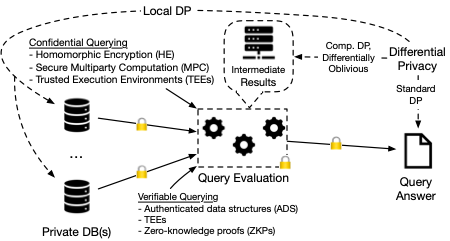
\includegraphics[bb = 0 0 220 118]{submissions/submission1/figs/pets-workflow.png}
        \caption{ Trustworthy DBs  in the query lifecycle}
    \label{fig:pets-workflow}
\end{wrapfigure}




\subsection{Query Lifecycle}

Figure~\ref{fig:pets-workflow} shows the broad steps with which a database system  evaluate a query and where they integrate assorted privacy and security-enhancing techniques into this workflow.  This figure is inspired by~\cite{secretflow2024survey}.  The dotted lines denote steps in the process that may leak information about a database's private records.  We expect  the initial input databases from one or more {\em data providers} or {\em data owners} are correct and complete at setup time.  A {\em clients} queries the records of one or more private databases.  The party computing the query answer\textendash this could be the data owner themselves, an untrusted cloud service provider used for outsourcing or others\textendash may have access to this information leakage.   We delve into specific trustworthy database architectures and the \sandp-preserving techniques that power them in the upcoming sections.    




\begin{figure}
\centering
    \subfloat[Client-Server]{
    \label{fig:arch:client-server}
    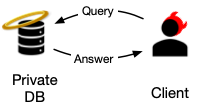
\includegraphics[bb= 0 0 113 65]{submissions/submission1/figs/client-server.png}}
    \hfill
    \subfloat[Outsourced Storage]{
    \label{fig:arch:outsourced-storage}
    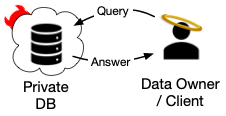
\includegraphics[bb= 0 0 113 65]{submissions/submission1/figs/outsourced-storage.png}}
    \hfill
    \subfloat[Private Data Federation]{
    \label{fig:arch:private-data-federation}
    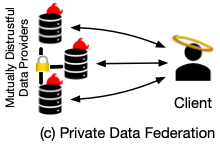
\includegraphics[bb= 0 0 113 65]{submissions/submission1/figs/private-data-federation.png}}  
    \hfill
    \subfloat[Outsourced  Computation]{
    \label{fig:arch:outsourced-computation}
    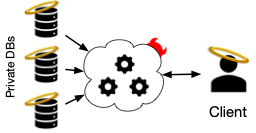
\includegraphics[bb= 0 0 113 65]{submissions/submission1/figs/outsourced-computation.png}}  
    \caption{Reference architectures for trustworthy database systems.}
    \label{fig:arch}
\end{figure}



\subsection{Trustworthy DBMS Architectures and Roadmap}
\label{sec:arch}

Throughout this text, we will reference several common architectures for query evaluation.  In this section, we will describe trustworthy database systems in terms of the  four architectures shown in Figure~\ref{fig:arch}. Our goal is to provide a  guide for future systems builders in selecting the most suitable one for their setting.  Admittedly, these frameworks are partially overlapping. We break them up as shown for ease of exposition.
 
A {\em client-server} architecture simply enables the client to send their  \query to the server with a private database and receive its answer, \answer as in Figure~\ref{fig:arch:client-server}.    For example, if the client is untrusted and the data provider is trusted, then the latter might protect their query answers from reconstruction by returning noisy versions of the true query answer using differential privacy.  We will cover this approach in Section~\ref{sec:dp}. 


The {\em outsourced storage} architecture, depicted in Figure~\ref{fig:arch:outsourced-storage}, starts with one or more untrusted cloud servers that have ample storage and limited compute resources. A data owner or trusted client outsources their storage operations to this platform to keep their data confidential.   These systems support a key-value store-esque interface. This is challenging because even when the database is stored encrypted, side-channel information such as memory access patterns can reveal some or all of the DB's contents~\cite{grubbs2016breaking,kellaris2016generic,markatou2019full}.  We introduce oblivious RAM in Section~\ref{sec:oram}; it is the main starting point for systems in this space.   If the client seeks only verifiable results, and they have access to more compute power on the server side,  they  might engage in verifiable querying as described in Section~\ref{sec:verifiable}.


The {\em private data federation} (PDF), shown in Figure~\ref{fig:arch:private-data-federation}, enables two or more mutually distrustful parties to compute \answer over the union of their private records without disclosing their private records to anyone.  This secure query evaluation may take place within cryptographic protocols evaluated among the data providers, described in Section~\ref{sec:oblivious} or in trusted hardware, as detailed in Section~\ref{sec:tees}.  


The {\em outsourced computation} setting in Figure~\ref{fig:arch:outsourced-computation} is when one or more data providers outsource their storage to the untrusted cloud and they delegate all query evaluation to this platform.  Here, the client and data providers are both trusted.  We discuss approaches to solving this challenge in Section~\ref{sec:secure}.  Similar to the PDF, platforms can securely compute in hardware or software.  This setup introduces another option: homomorphic encryption, or computing over encrypted data, as described in Section~\ref{sec:he}.

\section{Secure Query Processing}
\label{sec:secure}

In this section, we will examine techniques for query processing on outsourced databases, Figure~\ref{fig:arch:outsourced-computation}, and private data federations, Figure~\ref{fig:arch:private-data-federation}.   We group together these two architectures because there is strong overlap in their approaches and we highlight their differences we go along. We start with the strongest guarantee, oblivious querying, and then introduce popular relaxations to this. 

\subsection{Oblivious Querying}
\label{sec:oblivious}

A program is {\em oblivious} if its data access patterns and instruction traces are independent of their private input data.   \cut{An oblivious program's control flow does not change as a function of its private inputs.}  Oblivious algorithms prevent an attacker from inferring information about a database by observing its queries as they are evaluated.  An obliviously-executed query divulges nothing about its private inputs, except that which can be deduced from its results.

Researchers prove that a program is oblivious using the ``real world, ideal world'' paradigm~\cite{Canetti2001}.  Say that we are computing query  \query with mechanism \mechanism over database \db and there exists a probabilistic polynomial time simulator, $Sim$ that receives \db', an arbitrary database that is not \db but shares its schema and table cardinalities.   The observable traces of \mechanism should be computationally indistinguishable from those of $Sim$.  In other words, $Traces(\mathcal{M}, \mathcal{D}) \equiv Sim(\mathcal{M}, \mathcal{D}')$.  This paradigm makes it possible to compose independently developed building blocks, such as the oblivious query operators, into a query plan with strong end-to-end guarantees.  

There are a few common mechanics in oblivious database operators~\cite{bater2017smcql, zheng2017opaque,volgushev2019conclave,liagouris2023secrecy,ant2024scql}.  To keep their instruction traces oblivious to their private inputs, these programs evaluate both branches of private if-then statements, retaining only the one indicated by its secret conditional.  Similarly, they do not admit early termination of loops.  They conceal the selectivity of database operators with {\em dummy tuples} that replace rows that would be filtered out in an operator so that a curious observer cannot deduce anything  about a function's input data.  These engines typically represent this feature with a {\em dummy tag} or bit appended to each row  denoting whether it should be included in any subsequent calculations.  For example, an oblivious filter visits every row in a table and  applies its private predicate.   If the row satisfies the selection criteria, the oblivious if-then will update the row's dummy tag.  Otherwise,  it will simply overwrite the dummy tag with its previous value to remain oblivious.  We will describe oblivious database operators in detail in Section~\ref{sec:ops}.


Oblivious querying incurs a substantial performance penalty because its operators hide their data access patterns and any data-dependent changes in their control flow. With no additional info, queries with cascading joins must pad their output to the maximum possible size (the cross-product of their inputs) to conceal their selectivity.  Cumulatively, leads to a blow-up in their cardinalities increasing the cost of any subsequent computation.   As such, many oblivious database operators engage in selective information disclosure such as revealing the true cardinality of joins~\cite{krastnikov13efficient, zheng2017opaque} by default while offering full-padding  if desired.  If this is the root (last) operator in a query tree and the parties will receive \answer, then this is a sensible trade-off.  This picture gets more complicated if it is an intermediate result.


{\em Secure multiparty computation} (MPC)~\cite{goldreich1987mpc,lindell2021mpc} enables two or mutually distrustful parties to jointly compute over their private inputs obliviously.  Although early applied MPC protocols often implemented a special-purpose function (such as linear regression) to tackle the breathtaking overhead associated with general-purpose protocols, most modern systems compile their program logic into circuits~\cite{marcella2019sokmpccompilers}.  These {\em garbled circuits} reduce \query  into a series of gates, e.g., AND and XOR gates.  The protocol evaluates the circuit obliviously by traversing it in topological order.  They provide a Turing complete springboard for evaluating ad-hoc queries.   Some protocols use arithmetic gates instead of logic ones.   Performing all private computation within garbled circuits makes it possible to seamlessly compose the security guarantees of multiple, independently-developed components into a single proof under universal composability~\cite{Canetti2001}. 


\shortsection{Private Data Federations} There is a growing need to analyze information from multiple sources through a unified querying interface while addressing privacy concerns and complying with numerous privacy laws. A PDF, as  in Figure~\ref{fig:arch:private-data-federation}, integrates multiple autonomous database systems owned by mutually distrustful parties to query them as if they were a single query engine.  PDFs offer a shared schema that has table definitions agreed upon by all data providers at setup time.  It specifies the security level needed for each column.  Many PDF frameworks evaluate their queries under MPC.    This ensures that no unauthorized data is disclosed to other data providers participating in a secure query, while also minimizing the operations that \mechanism must perform under MPC by pushing them down for local evaluation~\cite{bater2017smcql, volgushev2019conclave, liagouris2023secrecy}.  


Data providers store private data in their own databases and compute query outputs in a privacy-preserving manner.  In PDFs, the process operates as follows: the client translates \query into the corresponding cryptographic protocols with which they will execute it.  They then send these instructions to all participating data providers.  The data providers then locally compute any public query operators  over their private records.  They then encode their selected private input rows for the operators that require secure, distributed evaluation over their unioned intermediate results.  They execute their oblivious operators by passing encrypted messages among themselves.  The data providers then send their share of \answer to the client over an encrypted link.  After receiving shares from all of the computing parties, the client assembles \answer. 

There are numerous threat models for MPC protocols, and they are detailed in~\cite{lindell2021mpc}.    A {\em semi-honest} party adheres to the protocols, but may attempt to learn additional, unauthorized information from observing the MPC protocol.  Semi-honest database systems include SMCQL~\cite{bater2017smcql}, Conclave~\cite{volgushev2019conclave}, and Hu-Fu~\cite{tong2022hu}. On the other hand, a {\em malicious} party both seeks to reveal information about a query's private inputs and they may deviate from the MPC protocol arbitrarily.  Senate~\cite{poddar2021senate} implements a PDF in the maliciously secure setting.  Some engines are starting to support multiple protocols or mixed models by compiling queries into abstract circuits (or methods) and applying different protocols for different settings.  SCQL~\cite{ant2024scql} and VaultDB~\cite{rogers2022vaultdb, vaultdb} take this approach.  Naturally, protocols with stronger guarantees incur more overhead for query evaluation, and this design choice depends on the setting in which they run.

\shortsection{Outsourced Computation}  MPC facilitates querying over the unioned data of 2+ independent private DBs.  We need one more step to extend this technology to the outsourced computation setting in Figure~\ref{fig:arch:outsourced-computation}.  To distribute trust over multiple outsourced hosts, a client may  {\em secret share} their private inputs and send shares of them to all computing parties.  Here no  party can reconstruct the secret unless the party colludes with a subset of parties. Before starting to evaluate \query's garbled circuits,  the parties participate in an {\em oblivious transfer} protocol to encode their data as wire labels for its logic gates.   This process is analogous to public-key cryptography where at the end of it each party holds an encrypted copy of the database without access to the key with which to decrypt it and none has access to the plaintext data except its initial owner.   


Platforms in the outsourced computation model have also been adopting MPC protocols.  The earliest work (to the best of our knowledge) in this space computed aggregates semi-honestly under 3-party computation~\cite{bogdanov2008sharemind}.  SDB~\cite{wong2014secure,Zhian2015SDB} created a hybrid model where the private data is secret-shared among the data owner and the cloud service provider.  For the semi-honest setting, Secrecy~\cite{liagouris2023secrecy} supports 3-party secure computation over ad-hoc SQL queries.     RESCU-SQL~\cite{li2023rescu} uses maliciously secure, $n$-party MPC protocols to protect outsourced data in the zero-trust cloud.  




\subsection{Oblivious RAM for Outsourced Storage}
\label{sec:oram}

We now turn our attention to the outsourced storage setting shown in Figure~\ref{fig:arch:outsourced-storage} in Section~\ref{sec:arch}.  Here, the client wishes to outsource the of their private database to the untrusted cloud.  If they simply encrypted their data and issued read and write requests against the specific records as they access them, then this will expose their data access patterns and make their data vulnerable to side-channel leakage attacks~\cite{kellaris2016generic, naveed2015inference, grubbs2016breaking}.  Unless otherwise specified, these systems have a key-value store-style API.   {\em Oblivious RAM}~\cite{goldreich1987oram} transforms a client's read and write requests into ones that are independent of their true memory access patterns. When a client requests a block, $b_i$, from their database, the ORAM rewrites it as a series of reads and writes that 1) shuffle their storage, and 2) pad their request with dummies to conceal the position of their request in the database.    This makes the distribution of their I/O requests oblivious to their true memory access patterns.  It also prevents an adversary from deducing the frequency of accesses to a specific $b_i$.  

Early work in outsourced storage centered on ORAM constructions themselves, with tree-based ones~\cite{stefanov2013pathoram, ren2015constants} emerging as the dominant paradigm in practice.  Several systems have generalized this work to distributed ORAMs, including Shroud~\cite{lorch2013shroud}, ObliviStore~\cite{stefanov2013oblivistore}, and TaoStore~\cite{sahin2016taostore}.  Snoopy~\cite{dauterman2021snoopy} integrates trusted hardware into their design to parallelize oblivious reads and writes.   Whereas ORAM makes all access requests indistinguishable from one another,  {\em frequency smoothing} relaxes this requirement to make the frequency with which individual $b_i$s are requested uniform.  Waffle~\cite{maiyya2023waffle} and Pancake~\cite{grubbs2020pancake} are examples of this approach. They do so by replicating popular objects and padding their I/O requests with dummies. 


The systems described above are all linearizable; they reason about concurrency at the granularity of one object at a time.  Additional mechanisms are needed for ACID transactions.   Obladi~\cite{crooks2018obladi} is an ORAM-backed storage engine that parallelizes ACID transactions on untrusted ORAM servers.  Treaty~\cite{giantsidi2022treaty} is a natural extension of this work obviates the need for a trusted proxy with trusted hardware.


\subsection{Homomorphic Encryption for Outsourced Computation}
\label{sec:he}

{\it Homomorphic encryption} (HE)~\cite{gentry2009fully} enables a system to compute over encrypted data without decrypting it.    HE and MPC are close cryptographic cousins.  Rather than distributing trust over multiple parties, HE enables data owners to outsource their operations to one host with a variation of the outsourced computation architecture in Figure~\ref{fig:arch}.  Here, the data provider encrypts their records and uploads them to the untrusted cloud (without providing the decryption key) and the client issues queries against the encrypted databases.   Whereas MPC enables parties to pipeline their circuit evaluation, i.e., compute each gate and discard intermediate wire labels when they are no longer needed, HE protocols evaluate a materialized circuit to produce \answer and send it to the client.  This is more efficient for straightforward operators such as filter, but may reveal scalability challenges for ones with deeper circuits such as aggregating over a large group of tuples.  Fully homomorphic encryption (FHE)  support circuits, and thus ad-hoc queries, without leaking information about the encrypted data.  FHE has a very high performance cost, typically several orders of magnitude slower than running in plaintext.  These schemes have seen limited adoption in databases in practice with the only known implementation for databases targeting aggregation alone~\cite{ren2022heda}.  HE has several relaxations to bridge this performance gap.  Some partially homomorphic encryption (PHE) schemes offer better performance in exchange for reduced security guarantees, such as order preserving encryption~\cite{boldyreva2009order,agrawal2004order} and deterministic encryption~\cite{boldyreva2008notions, bellare2008deterministic}.  Others support reduced expressiveness with higher performance, such as additive HE~\cite{paillier1999public} and multiplicative HE~\cite{elgamal1985public,rivest1978method}.

Database researchers have invested substantial research effort into bringing these encryption schemes to outsourced databases with a variation of the architecture in Figure~\ref{fig:arch:outsourced-computation}.  The data owner encrypts \db using HE and uploads them to the untrusted cloud server.  The client submits \query to the server and it computes \answer over its encrypted copy of \db.  ~\cite{agrawal2004order} introduced order-preserving encryption for answering database queries.  CryptDB~\cite{popa2011cryptdb}
and Monomi~\cite{tu2013processing} targeted HE for outsourced databases for OLTP and OLAP workloads, respectively.  The latter identified lightweight mechanisms for moving some of the query evaluation client-side to circumvent the performance limitations of FHE.  Unfortunately, these PHE schemes have substantial side-channel leakage associated with executing queries over them~\cite{naveed2015inference, bindschaedler2017tao}.  This is similar to the issues we described for non-oblivious access to outsourced storage above.  SEAL~\cite{demertzis2020seal} tackles some of this leakage with adjustable leakage that hides $\binom{n}{k}$ bits out of a search key by introducing a generalization of ORAM.


\subsection{Trusted Execution Environments for Outsourced and Federated Querying} 
\label{sec:tees}

Trusted Execution Environments, or TEEs, create an isolated computing platform within an untrusted computer using trusted hardware.  They have encrypted private memory with which they runs sealed code that is confirmed to be only the code given by the client or a proxy thereof (such as a trustworthy DBMS).  Hence, code run within TEEs are verifiable by virtue of running within a secure enclave, such as Intel SGX~\cite{dinh2019everything} and ARM TrustZone~\cite{pinto2019demystifying}.   Clients  delegate their program executions to trusted hardware, safeguarding their private data without the need for encryption. The main advantage is its efficiency, as it avoids the significant computational and communication overhead typically incurred by cryptographic primitives, making it more practical for real-world scenarios. Secure enclaves alone are not a panacea. For example, instruction traces leak memory access patterns, allowing eavesdroppers to infer private data from them~\cite{kellaris2016generic,markatou2019full}.

TEEs are seeing increased use for evaluating queries over confidential data  the cloud or outsourced computation in Figure~\ref{fig:arch:outsourced-computation}.  First-generation systems relied on software-hardware co-design to build TEEs with bespoke algorithms for query evaluation such as TrustedDB~\cite{bajaj2011trusteddb} from IBM and Microsoft's Cipherbase~\cite{arasu2013orthogonal}.  As SGX and other enclaves became widely available and cloud-ready, researchers created secure enclave extensions to well-known DBMSs.  For example, StealthDB~\cite{vinayagamurthy2019stealthdb} builds atop PostgreSQL and EnclaveDB~\cite{priebe2018enclavedb} runs within Hekaton.  In addition, since the resident host running the enclave can observe its memory access patterns, researchers have been building oblivious algorithms for use inside the TEE such as ObliDB~\cite{eskandarian2019oblidb} and Opaque~\cite{zheng2017opaque}.  This approach has also been appearing in TEE-based PDFs such as~\cite{dave2020oblivious}. 





\section{Differential Privacy} 
\label{sec:dp}

If the client is untrusted, the data provider may call for guarantees that prevent them from using query answers to infer information about their private input records. Speaking informally, {\em Differential Privacy} (DP) ~\cite{dp2006, dwork2008differential} protects private data from construction attacks by injecting carefully calibrated noise into their query answers to control their resulting information leakage before returning them to the client.   An algorithm satisfies differential privacy if its output is approximately the same over a database, \db, as it would be over a neighboring database differing by one record, \db'. This workflow, of a data provider or trusted curator noising query answers before releasing them to the client, is known as {\em Standard DP} or SDP~\cite{wagh2021dp}.     More broadly, if a secure database reveals precise, un-noised query answers, this creates unbounded information leakage~\cite{kifer2011no}.  SDP works on the client-server model in Figure~\ref{fig:arch:client-server}. 

Before answering their first query over \db, the data owner selects a privacy budget, \eps, with which they limit the information they leak in aggregate to the client or clients by answering their queries.  Recall that $\mathcal{R} := \mathcal{M}(\mathcal{D})$.   In its simplest form, if the client queries a private database $n$ times with mechanisms $\mathcal{M}_1, \ldots, \mathcal{M}_n$, and $\mathcal{M}_i$ has $\epsilon_i$, their net privacy loss is $\sum_{i=1}^n \epsilon_i$.  Researchers have proposed several frameworks for designing efficient DP mechanisms~\cite{johnson2020chorus, zhang2018ektelo, wang2021dpgen}.  Also, the database community has invested significant research effort into automatically deriving SDP answers to SQL queries with robust e2e  privacy guarantees ~\cite{ann2011airavat,mcsherry2009privacy,proserpio2014calibrating,johnson2018towards,kotsogiannis2019architecting, kotsogiannis2019privatesql}.



Choosing \eps for a given database and query workload reveals a trade-off between utility and privacy.  A larger \eps means that \mechanism will inject less noise into \answer.  In other words, more accurate query answers result in a greater privacy loss for \db.   Selecting an \eps with sufficient data protection while producing useful query answers is a challenging topic~\cite{lee2011much} and the subject of ongoing research~\cite{dwork2019differential, li2023towards, near2023guidelines}.  A conservative heuristic is to restrict $\epsilon$ to values less than or equal to one~\cite{wood2018differential}.

\subsection{Computational Differential Privacy} One major shortcoming of SDP is that assumes there is a single trusted data curator noising \answer.   \cut{It is attractive because its guarantees are information-theoretic.}  Computational DP (CDP)~\cite{beimel2008distributed, mironov2009computational} relaxes SDP's strong information-theoretic guarantees to a weaker, probabilistic polynomial time adversary in exchange for less noisy results and support for distributed data.   CDP quantifies information leakage when two or more parties are computing a function over their encrypted and unioned private inputs, $\mathcal{D}_*$.    It frames information leakage about \mechanism's intermediate results as a differentially private view of $\mathcal{D}_*$ and assigns some share of the privacy budget to it.    For example, if we are computing a CDP filter $\mathcal{R} := \sigma(\mathcal{D})$ we may start by running the oblivious evaluation described above.   We then generate a noisy version of its true output cardinality {\em within} the oblivious algorithm for release, $|\widetilde{\mathcal{R}}|$ and obliviously delete dummy rows.  This will make any parent operators run faster because they compute over fewer dummies. 

CDP introduces a third dimension to our DP trade-off:  performance.
If we allocate more privacy to computation, the client may get their query answer faster but with reduced accuracy because we spend some privacy releasing information about \mechanism's intermediate results, i.e., its noisy intermediate cardinality.  There's been significant research interest in using CDP to accelerate privacy-preserving query evaluation in PDFs~\cite{bater2018shrinkwrap, bater2020saqe,he2017composing}. 


CDP  extends to the outsourced storage setting.  Allowing an untrusted cloud service provider to view noisy versions of the client's memory access patterns enables this trade-off on efficiency and privacy.   DP-ORAM~\cite{wagh2018differentially} relaxes ORAM's full-oblivious guarantees to CDP ones.    $\epsilon$psolute~\cite{kellaris2017accessing, bogatov2021varepsilonpsolute} parallelizes CDP I/O requests among multiple ORAMs.   CDP has also been used to speed up outsourced computation for analytics~\cite{roy2020cryptepsilon} and for querying growing databases~\cite{zhang2023longshot, wang2022incshrink,wang2021dp} in the untrusted cloud.  



\subsection{Differential Obliviousness}
 Another DP relaxation gaining traction in the database community is differential obliviousness~\cite{chan2022foundations,chu2021differentially, qin2022adore, qiu2023doquet} (DO).   A DO algorithm offers a DP view of its memory traces by leaking approximate versions thereof.   This is related to CDP, with the latter approximating discrete views of \db.  To continue with our filter running example, a simplified version of the DO filter in~\cite{qin2022adore} partitions \db into batches of length $B$ where $B$ is polylog of $|$\db$|$. In lieu of running an oblivious filter, it writes to the output buffer of \answer one batch at a time maintaining a cursor for these writes.  For each block $b_i$ it computes a DP approximation of its prefix sum (how many rows are selected), this provides a range of the count of the rows $b_i$ will emit to \answer.  It then writes to $B$ slots in the output buffer with a mix of real and dummy rows and advances the cursor to the position indicated by the lower bound of its DP prefix sum. 
 
 DO strikes a balance between full-oblivious ones and ones with unbounded information leakage.   It admits secure algorithms with performance properties comparable to streaming or pipelined operators and it boasts better cache efficiency than approaches that materialize their entire \answer before noising it.     On the other hand, DO mechanisms are non-trivial compose~\cite{zhou2023theory}, and they need to maintain the notion of neighbor-preserving differentially oblivious datasets between an operator's input and output relations to compose a DAG of them.  Addressing this challenge is a topic of ongoing research.

\subsection{Local Differential Privacy}

  One more approach to limiting information leakage from querying private data is injecting noise into the private data before querying it.  Local DP~\cite{xiong2020comprehensive} (LDP) removes the need for a trusted data curator by noising it one row at a time.  There has been considerable research in incorporating this into database operations~\cite{cormode2018privacy,gu2019supporting,roth2020orchard,wang2017locally,xu13collecting}.  This is different from DP synthetic data generation~\cite{cai2023privlava,ge2021kamino,machanavajjhala2008privacy}, which creates a new dataset with values that mimic the distribution of a private one.  


LDP is attractive for aggregating ``wisdom of the crowd'' statistics, such as collecting new words and phrases for auto-complete as they enter the popular lexicon and identifying software bugs from noisy bug reports.  It also frees data collectors from the liability of storing raw user data, which may garner subpoenas or attempts to steal it.  Also, since the data are noised upfront,  clients may query it as many times as they wish without eroding the privacy budget.  On the other hand, because the data are perturbed one row at a time, the algorithm needs to add $O(\sqrt{n})$ to each entry for $n$ individuals contributing to \db, whereas SDP would simply noise the true count independent of the participant count~\cite{wagh2021dp}.




\section{Verifiable Querying}
\label{sec:verifiable}

Data owners are increasingly outsourcing their data management to the untrusted cloud.   With {\em verifiable computing} when an untrusted server answers a client query \query with \answer over a private database \db, they participate in a protocol to convince the client (with high probability) that \answer is correct and complete.   Here we have two participants: a prover \prover, the cloud service provider, and a verifier \verifier, the client.   If $\mathcal{C}_{ver}(\mathcal{D})$ is a function with which \prover and \verifier authenticates $\mathcal{R}$ with the following guarantees:
\vspace{-0.2cm}
\begin{itemize}
    \item Completeness.  If \prover faithfully executes \query then $ \mathcal{C}_{ver}(\mathcal{R})=1$.  \prover accepts honest proofs.
    \vspace{-0.3cm}
    \item Soundness.  If \prover outputs an incorrect \answer,  $Pr[\mathcal{C}_{ver}(\mathcal{R})=1] \leq \epsilon$, where $\epsilon$ is a negligible probability.
\end{itemize}
\vspace{-0.2cm}
Systems such as IntegriDB~\cite{zhang2015integridb}, Concerto~\cite{arasu2017concerto}, CorrectDB~\cite{bajaj2013correctdb}, VeriDB~\cite{zhou2021veridb} and vSQL~\cite{zhang2017vsql} use VC to guarantee data integrity for querying.  


There are several approaches to creating verifiable query answers.  With an {\em Authenticated Data Structure}, \prover generates a proof that accompanies \answer to validate that it is complete and sound.  The two main methods that instantiate ADS are tree-based and signature-based methods.  The tree-based method builds a binary tree for a database, where each leaf node stores a digest about tuples in the database, and its internal nodes are digests that summarize its children.   When evaluating a query, the database sends the query answer along with a set of digests for the relevant nodes to the client, who has the digest of the root node, to verify the answer by reconstructing the path to match the root node. IntegriDB is such a system that applies a dynamic tree-based ADS tailored for a specific set of queries, allowing the client to query and verify $\mathcal{R}$ using precomputed digests aided by the accompanying proof. On the other hand, signature-based methods constructs a set of signatures for tuples in the database. During query evaluation, the cloud-hosted database sequentially collects a set of signed tuples that it accesses. Then the client verifies each tuple that no unwanted tuple is included and no necessary tuple is missed.

Similarly, Concerto, CorrectDB and VeriDB utilize ADS-based verifiable computing to verify their queries, but they compose ADSs with TEEs benefit from greater efficiency than working solely with cryptographic primitives (see Section~\ref{sec:tees}). Concerto is a concurrent key-value store, while VeriDB and CorrectDB support ad-hoc SQL queries for relational databases.

With {\em interactive proofs}~\cite{zhang2015integridb}, \prover and \verifier  work together to confirm the authenticity of  a statement $C(w)$ over a witness $w$ via multiple rounds of challenge-response messages, thereby incrementally ensuring correctness and soundness.  This VC approach is an alternative to ADS.  Similar to MPC, these proofs work in the circuit paradigm\textendash they express their logic as gates. In our context, $w$ is the private database $\mathcal{D}$.  \prover and \verifier interactively establish $w$ as a commitment of \db.  This forms the immutable starting point for \prover's proof for \query. Upon receiving the last respone $\mathcal{R}$ from \prover, \verifier accepts it iif $\mathcal{C}_{ver}(\mathcal{R})=1$. In other words, \verifier rejects immediately if it receives any unconvincing response from \prover during the interaction. In contrast to ADS-based systems mentioned above, vSQL is more expressive by supporting a wider range of SQL queries through IPs. Although interactive proofs incur significant communication overhead between the client and server, vSQL operates with nearly the same efficiency as those systems.

However, the client might attempt to obtain extra information that it is not authorized to access. For example, VC-backed systems with ADS and interactive proofs ensure the integrity of an outsourced database, but they reveal the data owner's records to the cloud service provider. Moreover, TEE-based systems may leak memory access patterns through program traces, as discussed in Section~\ref{sec:tees}. Therefore, the aforementioned systems are inadequate to protect private data on an untrusted server. For this we need to add one more guarantee to our stack, {\em zero knowledge}~\cite{goldreich1991zkp,goldwasser1985zkp}:
\vspace{-0.2cm}
\begin{itemize}
    \item Zero knowledge. If  $\mathcal{C}_{ver}(\mathcal{R})=1$, \verifier learns nothing other than the fact \answer was computed correctly.
\end{itemize}
\vspace{-0.2cm}
To provide such a stronger guarantee in verifiable querying, the database community has adopted {\it zero-knowledge proofs} for SQL queries~\cite{zhang2017vsqlzk, li2023zksql} to offer privacy and confidentiality for query answering.  This guarantee is similar to the one we saw for obliviousness: \verifier learns nothing more than \answer and that which can be deduced from it.  The main difference here is that \prover is able to prove  properties of intermediate query results, such as proving a sorted list of tuples is monotonically increasing, rather than evaluating the entire program logic in circuits. Overall, \zkps enable \prover to convince \verifier of the query answer \answer by authenticating it with a proof, without revealing any additional information beyond the information that could be derived from \answer. This means we could simultaneously address both data integrity and data privacy for the outsourced database.



There are two main flavors of zero-knowledge proofs: {\it interactive} and {\it non-interactive} \zkps.  Interactive ones are analogous to MPC, where \prover and \verifier verify a circuit one gate at a time using pipelined gates. In contrast to IPs, \zkps divulges no additional information about $w$ beside the truth of $C(w)$ to \verifier while IPs do not hide $w$ from \verifier.

Zero-knowledge extension of vSQL~\cite{zhang2017vsqlzk} and ZKSQL~\cite{li2023zksql} utilize interactive \zkps. While the former remains theoretical as a pioneering effort, ZKSQL optimizes computationally expensive operators for practical use, such as sort and join, reducing their respective complexities from $O(n \log n)$ and $O(n^2)$ to $O(n)$. This optimization is achieved through \prover's local computation and interactive verification with ZK set operations, where the set-based proofs are represented by polynomials instead of circuits, unlike conventional interactive \zkps. For example, in sorting, we can only check if the result contains the same tuples as the unsorted table using ZK set equality when the result confirms to be monotonically increasing or decreasing.

Conversely, non-interactive ones construct a monolithic circuit for their query in a single step, providing a single proof that \prover sends with \answer. They require no additional interaction between \prover and \verifier and are widely used in blockchain applications. However, a significant drawback is the large proof size, which can be memory-intensive due to the one-shot construction. Despite potentially being more efficient than the interactive ones due to reduced communication overhead, we do not recommend this approach for systems aiming to scalability.

In addition to the single prover-verifier system, there are also distributed or decentralized verification systems that build atop blockchains~\cite{el2019blockchaindb, allen2019veritas, peng2020falcondb,yueglassdb}. They guarantee auditability, accountability, and traceability on the ledger during data sharing across mutually distrustful parties, but their combined records are largely accessible to all participants on the chain thus they are beyond the scope of this paper.

\section{Privacy-Preserving Database Operators}
\label{sec:ops}

This section introduces privacy-preserving database operators.  They are crucial for secure and privacy-preserving query evaluation. 


We start with oblivious operators.  Recall from Section~\ref{sec:oblivious} that they guarantee that their memory access patterns and program traces do not disclose any information about their private inputs.   These operators ensure that even if an adversary knows \query and observes its execution under \mechanism, they learn no additional information from participating in its evaluation.~\cite{arasu2014oblivious} introduced the earliest formal definitions for efficient algorithms for oblivious query processing.  This paper covers approaches for selections, joins, and group-by aggregation.  It was designed for use in TEEs, although no practical implementation of its results are forthcoming.  Since then, there has been a lot of excitement in the research community about creating efficient, oblivious algorithms for database operators~\cite{ant2024scql, bater2017smcql, krastnikov13efficient, zheng2017opaque}.  We will also touch upon operators that offer alternative privacy guarantees, such as CDP and DO from Section~\ref{sec:dp}.  We will mainly focus on joins in this survey because, in our experience, these tend to be the bottleneck for most secure query workloads.  In addition, joins have attracted the most research results to date in terms of operator algorithms proposed.

\subsection{Joins}

Table~\ref{tbl:joins} presents a comprehensive categorization of privacy-preserving join approaches. This considers several key dimensions: computational complexity, employed methods, type of leakage, number of participating parties, and supporting join types. Notably, the table organizes the joins based on their leakage, establishing distinct categories for oblivious joins, differentially oblivious joins, and differentially private joins. 


\begin{table}
    \centering
    \begin{tabular}{l|c|c|c|p{2.8cm}|c}
     {\bf Strategy}    & {\bf Complexity} &{\bf  Compute Method} & {\bf Leakage}  &{\bf  \# of Parties} & {\bf Join Type} \\
     \hline 
     Nested Loop & $O(n^2)$ & SH-2PC & Oblivious & 2:~\cite{bater2017smcql, vaultdb} & all \\
     
      &  &  SH-3PC & Oblivious  &  3:~\cite{volgushev2019conclave, liagouris2023secrecy} &  \\

      &  &  Mal-MPC & Oblivious  &  N:~\cite{li2023rescu} &  \\
     
      &  &  SH-2PC &   CDP &  2:~\cite{bater2018shrinkwrap, bater2020saqe} &  \\
       &  & TEE & Oblivious &  1:~\cite{li2008privacy}, $\geq2$:~\cite{dave2020oblivious}&  \\
       
     \hline
     NLJ w/semi-join & $(n \times RF)^2$ & SH-2PC & Oblivious & 2:  \cite{bater2017smcql}  & equi-join \\ 
    &  &SH-3PC  &  Oblivious  &  3:~\cite{chu2021differentially, liagouris2023secrecy} & \\ 
     \hline

    Index NLJ & $n \log ^2 n$ & ORAM & Oblivious & N:  \cite{chang2022towards}  & all \\ 
    \hline

    Sort-Merge Join & $n \log ^2 n$ & TEE & Oblivious & $\geq 1$: \cite{krastnikov13efficient, eskandarian2019oblidb, zheng2017opaque} & equi-join \\ 
                    &    & SH-3PC & Oblivious & 3:~\cite{li2024experimental} & \\
                    &    & TEE & DO & $\geq 1:$  \cite{chu2021differentially}& \\
                    \hline 
       PK-FK SMJ             & $n \log n$   & TEE & DO & $\geq 1$:~\cite{qin2022adore} & 1:n \\
     \hline
    
     Hash Join & $n$ & SH-3PC & Oblivious& 3:~\cite{mohassel2020fast} & equi-join \\ 
     \hline

     Hash SMJ & $n$ & SH-3PC & Oblivious& 3:~\cite{luo2024secure} & equi-join \\ 
     \hline

     PSI join & $n$ & SH-2PC & Oblivious & 2:~\cite{raghuraman2022blazing, wang2021secure}; & pk-pk \\
      & & Mal-2PC & Oblivious & 2:~\cite{raghuraman2022blazing} & pk-pk \\
      & $n \log n$  & SH-MPC & Oblivious & N:~\cite{ant2024scql} & equi-join \\
      & $n \ln \ln n$  & SH-MPC & CDP & N:~\cite{narayan2012djoin} & equi-join \\
      \hline
      
      Partition Join & $n \log ^2 n$   & TEE & Oblivious & N:~\cite{li2023soda} & equi-join \\
      & $n \log n$   & TEE & DO & $\geq 1$:~\cite{qiu2023doquet} & equi-join \\
    \end{tabular}
    \caption{Comparison of secure join algorithms.   }
    \label{tbl:joins}
\end{table}


\shortsection{Oblivious Join}
The most strict technique is fully oblivious join, which allows combining data from different sources without revealing sensitive information. Various algorithms have been evaluated in~\cite{li2024experimental} to determine their efficiency and security, as shown in table~\ref{tbl:joins}. The study reveals the overall efficiency ranking, wherein PSI emerges as the most efficient, followed by hash approaches. However, the efficiency of NLJ and SMJ can surpass others under high join selectivity. Additionally, optimal join order significantly improves efficiency, highlighting the importance of cost-based query optimization. 

\shortsection{DO Joins}
To improve efficiency, DO join permits a controlled degree of information leakage about the data while still providing meaningful privacy guarantees based on the relaxed notion of $(\epsilon, \delta)-$differential obliviousness. Key advancements in this area include the DO join~\cite{chu2021differentially}, Adore~\cite{qin2022adore}, Doquet~\cite{qiu2023doquet}, as shown in Table~\ref{tbl:joins}. Fully oblivious join algorithms are inefficient due to worst-case padding, resulting in significant performance overheads. The DO join algorithm addresses this by using $(\epsilon, \delta)-$DO~\cite{chan2022foundations}, a less strict privacy concept, to achieve efficient joins compared to insecure methods while preserving privacy. This approach provides meaningful privacy guarantees and proves new lower bounds on DO join algorithm performance. Adore employs a similar strategy with a sort-merge join but improves efficiency by using bucket oblivious sort, reducing the sorting complexity from bitonic sort's O($n \log^2(n)$) to O($n \log n)$. Additionally, Doquet optimizes join costs through a partitioning approach, significantly improving performance. 


\shortsection{CDP Joins} CDP joins provide strong privacy guarantees by ensuring that the inclusion or exclusion of any individual in the dataset trivializes the join operation's outcome. DJoin~\cite{narayan2012djoin} supports SQL-style join queries across multiple databases using two novel primitives: Blinded, Noised Private Set Intersection Cardinality (BN-PSI-CA) for private intersections with added noise to ensure differential privacy, and Denoise-Combine-Renoise (DCR) which combines noised subset sizes efficiently for privacy-preserving joins on distributed data. This results in an efficient join complexity. Shrinkwrap~\cite{bater2018shrinkwrap} addresses inefficiencies in PDF by leveraging computation differential privacy to reduce intermediate result padding. It integrates a cost model and privacy budge optimizer to balance privacy and performance. SAQE~\cite{bater2020saqe} scales PDF to handle large datasets by combining DP with approximate query processing. It introduces secure sampling algorithm that reduce computation costs and minimize the noise injected into query results.  


\subsection{Additional Operators}

We will now focus on additional operators and frameworks in the trustworthy database system landscape.

\shortsection{Oblivious Aggregate}
Oblivious aggregation computes summary statistics over a set of records without revealing how they are partitioned with a {\tt GROUP BY} clause. {\sc SAGMA}~\cite{hackenjos2020sagma} and {\sc OBSCURE}~\cite{gupta12obscure} represent two approaches to this challenge. {\sc SAGMA} supports secure aggregation grouped by multiple attributes under somewhat holomorphic encryption (SWHE). It allows the user to choose any combination of grouping attributes and privately maps rows to buckets, balancing storage and computational needs. However, {\sc SAGMA}'s main drawback is its need to store an exponentially growing set of monomials because its SWHE encoding supports only one multiplication operation~\cite{ren2022heda}. On the other hand, {\sc OBSCURE} encodes private rows using order-preserving secret sharing (OP-SS), which maintains data order securely while supporting repeated aggregation queries. {\sc OBSCURE} also introduces an oblivious result verification mechanism and demonstrates scalability to large datasets, addressing challenges faced by previous secret-sharing or MPC systems. However, {\sc OBSCURE}'s use of OP-SS is not inherently secure and is vulnerable to background knowledge attacks. 

\shortsection{Oblivious Filter}
 QFilter~\cite{mirabi2023qfilter} combines an Attribute-Based Access Control (ABAC) model with query processing over secret-shared data. This integration allows for fine-grained access control while preserving privacy. It handles aggregation SQL queries like ``count", ``sum", and ``avg", without requiring inter-server communication, thus securing against honest-but-curious adversaries. The system efficiently handles queries through string matching-based operators, rewriting SQL queries to embed access authorizations and filter unauthorized data during execution. However, QFilter's limitations include its inability to support more complex queries like ``min" and ``max" functions, ``group-by" clauses, or range queries, which limits its applicability in demanding data environments.

\shortsection{SODA}
SODA~\cite{li2023soda} introduces a collection of oblivious algorithms designed for distributed data analytics, including filter, aggregate, and binary equi-join operations. It improves upon previous systems like Opaque~\cite{zheng2017opaque} by minimizing data padding through a two-level bin-packing strategy. This approach effectively manages input redistribution and handles join product skewness. SODA further avoids expensive global sort primitives by employing low-cost pseudo-random communication to guarantee uniform data traffic. However, SODA does not address issues related to denial-of-service attacks or physical side-channel attacks. Additionally, it does not integrate hardware oblivious memory, which could further protect against side-channel vulnerabilities by hiding access patterns more effectively.

\shortsection{Differentially Oblivious Operators}
 Adore~\cite{qin2022adore} not only achieves differential obliviousness for joins, but it extends this guarantee to other database operators, like selection and aggregation, by working within secure enclaves. Doquet~\cite{qiu2023doquet} introduces a framework for DO range and join queries using private data structures.  It improves on the efficiency of Adore and oblivious algorithms on SGX.   Doquet also addresses access pattern leakage vulnerabilities that were present in Adore, ensuring a more secure implementation than that of its predecessor.   Both systems highlight the potential of DO to trade off on privacy and efficiency in query evaluation.


\section{Conclusions}
\label{sec:conclusion}

In this paper we surveyed the state-of-the art in security and privacy-preserving database systems.  We compared the properties of competing frameworks for trustworthy querying, such as secure computation vs trusted hardware for secure querying and authenticated data structures vs interactive proving for verifiable querying.  In addition, we described how differential privacy is making its way into nearly all of the steps in the query lifecycle.  We highlighted how composing these techniques reveals many subtleties in their \sandp guarantees, such as computational differential privacy over secure computation.  We closed with an exploration of how these techniques come together to create efficient, privacy-preserving database operators.

\begin{thebibliography}{140}
\itemsep=1pt
\begin{small}

\bibitem{agrawal2004order}
R.~Agrawal, J.~Kiernan, R.~Srikant, and Y.~Xu.
\newblock Order preserving encryption for numeric data.
\newblock In {\em Proceedings of the 2004 ACM SIGMOD international conference
  on Management of data}, pages 563--574, 2004.

\bibitem{allen2019veritas}
L.~Allen, P.~Antonopoulos, A.~Arasu, J.~Gehrke, J.~Hammer, J.~Hunter,
  R.~Kaushik, D.~Kossmann, J.~Lee, and e.~a. Ravi~Ramamurthy.
\newblock Veritas: Shared verifiable databases and tables in the cloud.
\newblock In {\em 9th Biennial Conference on Innovative Data Systems Research
  (CIDR)}, pages 1--9, 2019.

\bibitem{secretflow2024survey}
{Ant Group}.
\newblock A comprehensive comparison of various privacy-preserving
  technologies.
\newblock \url{https://www.yuque.com/secret-flow/admin/exgixt72drdvdsy3}.
\newblock Accessed: 2024-06-12.

\bibitem{ant2024scql}
{Ant Group}.
\newblock Secure collaborative query language.
\newblock \url{https://github.com/secretflow/scql}.
\newblock Accessed: 2024-06-13.

\bibitem{arasu2013orthogonal}
A.~Arasu, S.~Blanas, K.~Eguro, R.~Kaushik, D.~Kossmann, R.~Ramamurthy, and
  R.~Venkatesan.
\newblock Orthogonal security with cipherbase.
\newblock In {\em CIDR}, 2013.

\bibitem{arasu2017concerto}
A.~Arasu, K.~Eguro, R.~Kaushik, D.~Kossmann, P.~Meng, V.~Pandey, and
  R.~Ramamurthy.
\newblock Concerto: A high concurrency key-value store with integrity.
\newblock In {\em Proceedings of the 2017 ACM International Conference on
  Management of Data}, pages 251--266, 2017.

\bibitem{arasu2014oblivious}
A.~Arasu and R.~Kaushik.
\newblock Oblivious query processing.
\newblock {\em ICDT}, 2014.

\bibitem{bajaj2011trusteddb}
S.~Bajaj and R.~Sion.
\newblock Trusteddb: a trusted hardware based database with privacy and data
  confidentiality.
\newblock In {\em Proceedings of the 2011 ACM SIGMOD International Conference
  on Management of data}, pages 205--216, 2011.

\bibitem{bajaj2013correctdb}
S.~Bajaj and R.~Sion.
\newblock Correctdb: Sql engine with practical query authentication.
\newblock {\em Proceedings of the VLDB Endowment}, 6(7):529--540, 2013.

\bibitem{bater2017smcql}
J.~Bater, G.~Elliott, C.~Eggen, S.~Goel, A.~N. Kho, and J.~Rogers.
\newblock Smcql: Secure query processing for private data networks.
\newblock {\em Proc. VLDB Endow.}, 10(6):673--684, 2017.

\bibitem{bater2018shrinkwrap}
J.~Bater, X.~He, W.~Ehrich, A.~Machanavajjhala, and J.~Rogers.
\newblock Shrinkwrap: efficient sql query processing in differentially private
  data federations.
\newblock {\em Proceedings of the VLDB Endowment}, 12(3), 2018.

\bibitem{bater2020saqe}
J.~Bater, Y.~Park, X.~He, X.~Wang, and J.~Rogers.
\newblock {SAQE}: practical privacy-preserving approximate query processing for
  data federations.
\newblock {\em Proceedings of the VLDB Endowment}, 13(12):2691--2705, 2020.

\bibitem{beimel2008distributed}
A.~Beimel, K.~Nissim, and E.~Omri.
\newblock Distributed private data analysis: Simultaneously solving how and
  what.
\newblock In {\em Advances in Cryptology--CRYPTO 2008: 28th Annual
  International Cryptology Conference, Santa Barbara, CA, USA, August 17-21,
  2008. Proceedings 28}, pages 451--468. Springer, 2008.

\bibitem{bellare2008deterministic}
M.~Bellare, M.~Fischlin, A.~O’Neill, and T.~Ristenpart.
\newblock Deterministic encryption: Definitional equivalences and constructions
  without random oracles.
\newblock In {\em Advances in Cryptology--CRYPTO 2008: 28th Annual
  International Cryptology Conference, Santa Barbara, CA, USA, August 17-21,
  2008. Proceedings 28}, pages 360--378. Springer, 2008.

\bibitem{bindschaedler2017tao}
V.~Bindschaedler, P.~Grubbs, D.~Cash, T.~Ristenpart, and V.~Shmatikov.
\newblock The tao of inference in privacy-protected databases.
\newblock {\em Cryptology ePrint Archive}, 2017.

\bibitem{bogatov2021varepsilonpsolute}
D.~Bogatov, G.~Kellaris, G.~Kollios, K.~Nissim, and A.~O'Neill.
\newblock \ensuremath{\varepsilon}psolute: Efficiently querying databases while
  providing differential privacy.
\newblock In {\em Proceedings of the 2021 ACM SIGSAC Conference on Computer and
  Communications Security}, pages 2262--2276, 2021.

\bibitem{bogdanov2008sharemind}
D.~Bogdanov, S.~Laur, and J.~Willemson.
\newblock Sharemind: A framework for fast privacy-preserving computations.
\newblock In S.~Jajodia and J.~Lopez, editors, {\em Proceedings of the 13th
  European Symposium on Research in Computer Security.}, volume 5283 of {\em
  Lecture Notes in Computer Science}, pages 192--206. Springer
  Berlin/Heidelberg, 2008.

\bibitem{boldyreva2009order}
A.~Boldyreva, N.~Chenette, Y.~Lee, and A.~O’neill.
\newblock Order-preserving symmetric encryption.
\newblock In {\em Advances in Cryptology-EUROCRYPT 2009: 28th Annual
  International Conference on the Theory and Applications of Cryptographic
  Techniques, Cologne, Germany, April 26-30, 2009. Proceedings 28}, pages
  224--241. Springer, 2009.

\bibitem{boldyreva2008notions}
A.~Boldyreva, S.~Fehr, and A.~O’Neill.
\newblock On notions of security for deterministic encryption, and efficient
  constructions without random oracles.
\newblock In {\em Advances in Cryptology--CRYPTO 2008: 28th Annual
  International Cryptology Conference, Santa Barbara, CA, USA, August 17-21,
  2008. Proceedings 28}, pages 335--359. Springer, 2008.

\bibitem{cai2023privlava}
K.~Cai, X.~Xiao, and G.~Cormode.
\newblock Privlava: synthesizing relational data with foreign keys under
  differential privacy.
\newblock {\em Proceedings of the ACM on Management of Data}, 1(2):1--25, 2023.

\bibitem{Canetti2001}
R.~Canetti.
\newblock Universally composable security: A new paradigm for cryptographic
  protocols.
\newblock In {\em Proceedings 42nd IEEE Symposium on Foundations of Computer
  Science}, pages 136--145. IEEE, 2001.

\bibitem{chan2022foundations}
T.-H.~H. Chan, K.-M. Chung, B.~Maggs, and E.~Shi.
\newblock Foundations of differentially oblivious algorithms.
\newblock {\em ACM Journal of the ACM (JACM)}, 69(4):1--49, 2022.

\bibitem{chang2022towards}
Z.~Chang, D.~Xie, S.~Wang, and F.~Li.
\newblock Towards practical oblivious join.
\newblock In {\em Proceedings of the 2022 International Conference on
  Management of Data}, pages 803--817, 2022.

\bibitem{chicaiza2020application}
J.~Chicaiza, M.~C. Cabrera-Loayza, R.~Elizalde, and N.~Piedra.
\newblock Application of data anonymization in learning analytics.
\newblock In {\em Proceedings of the 3rd International Conference on
  Applications of Intelligent Systems}, pages 1--6, 2020.

\bibitem{chor1998private}
B.~Chor, E.~Kushilevitz, O.~Goldreich, and M.~Sudan.
\newblock Private information retrieval.
\newblock {\em Journal of the ACM (JACM)}, 45(6):965--981, 1998.

\bibitem{roy2020cryptepsilon}
A.~R. Chowdhury, C.~Wang, X.~He, A.~Machanavajjhala, and S.~Jha.
\newblock Crypt$\epsilon$: Crypto-assisted differential privacy on untrusted
  servers.
\newblock In {\em Proceedings of the 2020 ACM SIGMOD International Conference
  on Management of Data}, pages 603--619, 2020.

\bibitem{chu2021differentially}
S.~Chu, D.~Zhuo, E.~Shi, and T.~H. Chan.
\newblock Differentially oblivious database joins: Overcoming the worst-case
  curse of fully oblivious algorithms.
\newblock In {\em 2nd Conference on Information-Theoretic Cryptography}, 2021.

\bibitem{cormode2018privacy}
G.~Cormode, S.~Jha, T.~Kulkarni, N.~Li, D.~Srivastava, and T.~Wang.
\newblock Privacy at scale: Local differential privacy in practice.
\newblock In {\em Proceedings of the 2018 International Conference on
  Management of Data}, pages 1655--1658, 2018.

\bibitem{crooks2018obladi}
N.~Crooks, M.~Burke, E.~Cecchetti, S.~Harel, R.~Agarwal, and L.~Alvisi.
\newblock Obladi: Oblivious serializable transactions in the cloud.
\newblock In {\em 13th USENIX Symposium on Operating Systems Design and
  Implementation (OSDI 18)}, pages 727--743, 2018.

\bibitem{dauterman2021snoopy}
E.~Dauterman, V.~Fang, I.~Demertzis, N.~Crooks, and R.~A. Popa.
\newblock Snoopy: Surpassing the scalability bottleneck of oblivious storage.
\newblock In {\em Proceedings of the ACM SIGOPS 28th Symposium on Operating
  Systems Principles}, pages 655--671, 2021.

\bibitem{dave2020oblivious}
A.~Dave, C.~Leung, R.~A. Popa, J.~E. Gonzalez, and I.~Stoica.
\newblock Oblivious coopetitive analytics using hardware enclaves.
\newblock In {\em Proceedings of the Fifteenth European Conference on Computer
  Systems}, pages 1--17, 2020.

\bibitem{demertzis2020seal}
I.~Demertzis, D.~Papadopoulos, C.~Papamanthou, and S.~Shintre.
\newblock $\{$SEAL$\}$: Attack mitigation for encrypted databases via
  adjustable leakage.
\newblock In {\em 29th USENIX security symposium (USENIX Security 20)}, pages
  2433--2450, 2020.

\bibitem{dinh2019everything}
T.~Dinh~Ngoc, B.~Bui, S.~Bitchebe, A.~Tchana, V.~Schiavoni, P.~Felber, and
  D.~Hagimont.
\newblock Everything you should know about intel sgx performance on virtualized
  systems.
\newblock {\em Proceedings of the ACM on Measurement and Analysis of Computing
  Systems}, 3(1):1--21, 2019.

\bibitem{dp2006}
C.~Dwork.
\newblock {Differential Privacy}.
\newblock In {\em Automata, Languages and Programming}. Springer, 2006.

\bibitem{dwork2008differential}
C.~Dwork.
\newblock Differential privacy: A survey of results.
\newblock In {\em International conference on theory and applications of models
  of computation}, pages 1--19. Springer, 2008.

\bibitem{dwork2019differential}
C.~Dwork, N.~Kohli, and D.~Mulligan.
\newblock Differential privacy in practice: Expose your epsilons!
\newblock {\em Journal of Privacy and Confidentiality}, 9(2), 2019.

\bibitem{el2019blockchaindb}
M.~El-Hindi, C.~Binnig, A.~Arasu, D.~Kossmann, and R.~Ramamurthy.
\newblock Blockchaindb: A shared database on blockchains.
\newblock {\em Proceedings of the VLDB Endowment}, 12(11):1597--1609, 2019.

\bibitem{elgamal1985public}
T.~ElGamal.
\newblock A public key cryptosystem and a signature scheme based on discrete
  logarithms.
\newblock {\em IEEE transactions on information theory}, 31(4):469--472, 1985.

\bibitem{eskandarian2019oblidb}
S.~Eskandarian and M.~Zaharia.
\newblock Oblidb: oblivious query processing for secure databases.
\newblock {\em Proceedings of the VLDB Endowment}, 13(2):169--183, 2019.

\bibitem{ge2021kamino}
C.~Ge, S.~Mohapatra, X.~He, and I.~F. Ilyas.
\newblock Kamino: constraint-aware differentially private data synthesis.
\newblock {\em Proceedings of the VLDB Endowment}, 14(10):1886--1899, 2021.

\bibitem{gentry2009fully}
C.~Gentry.
\newblock Fully homomorphic encryption using ideal lattices.
\newblock In {\em Proceedings of the forty-first annual ACM symposium on Theory
  of computing}, pages 169--178, 2009.

\bibitem{giantsidi2022treaty}
D.~Giantsidi, M.~Bailleu, N.~Crooks, and P.~Bhatotia.
\newblock Treaty: Secure distributed transactions.
\newblock In {\em 2022 52nd Annual IEEE/IFIP International Conference on
  Dependable Systems and Networks (DSN)}, pages 14--27. IEEE, 2022.

\bibitem{goldreich1987oram}
O.~Goldreich.
\newblock Towards a theory of software protection and simulation by oblivious
  rams.
\newblock In {\em Proceedings of the nineteenth annual ACM symposium on Theory
  of computing}, pages 182--194, 1987.

\bibitem{goldreich1987mpc}
O.~Goldreich, S.~Micali, and A.~Wigderson.
\newblock How to play any mental game or a completeness theorem for protocols
  with honest majority.
\newblock In {\em Proceedings of the nineteenth annual ACM symposium on Theory
  of computing}, pages 218--229, 1987.

\bibitem{goldreich1991zkp}
O.~Goldreich, S.~Micali, and A.~Wigderson.
\newblock Proofs that yield nothing but their validity or all languages in np
  have zero-knowledge proof systems.
\newblock {\em Journal of the ACM}, 38(3):691--729, 1991.

\bibitem{goldwasser1985zkp}
S.~Goldwasser, S.~Micali, and C.~Rackoff.
\newblock The knowledge complexity of interactive proof-systems.
\newblock In {\em Proceedings of the seventeenth annual ACM symposium on Theory
  of computing}, pages 291--304, 1985.

\bibitem{grubbs2020pancake}
P.~Grubbs, A.~Khandelwal, M.-S. Lacharité, L.~Brown, L.~Li, R.~Agarwal, and
  T.~Ristenpart.
\newblock Pancake: Frequency smoothing for encrypted data stores.
\newblock In {\em 29th USENIX Security Symposium (USENIX Security 20)}, pages
  2451--2468, 2020.

\bibitem{grubbs2016breaking}
P.~Grubbs, R.~McPherson, M.~Naveed, T.~Ristenpart, and V.~Shmatikov.
\newblock Breaking web applications built on top of encrypted data.
\newblock In {\em Proceedings of the 2016 ACM SIGSAC Conference on Computer and
  Communications Security}, pages 1353--1364, 2016.

\bibitem{gu2019supporting}
X.~Gu, M.~Li, Y.~Cao, and L.~Xiong.
\newblock Supporting both range queries and frequency estimation with local
  differential privacy.
\newblock In {\em 2019 IEEE Conference on Communications and Network Security
  (CNS)}, pages 124--132. IEEE, 2019.

\bibitem{gupta12obscure}
P.~Gupta, Y.~Li, S.~Mehrotra, N.~Panwar, S.~Sharma, and S.~Almanee.
\newblock Obscure: Information-theoretic oblivious and verifiable aggregation
  queries.
\newblock {\em Proceedings of the VLDB Endowment}, 12(9), 2019.

\bibitem{hacigumucs2002executing}
H.~Hacig{\"u}m{\"u}{\c{s}}, B.~Iyer, C.~Li, and S.~Mehrotra.
\newblock Executing sql over encrypted data in the database-service-provider
  model.
\newblock In {\em Proceedings of the 2002 ACM SIGMOD international conference
  on Management of data}, pages 216--227, 2002.

\bibitem{hackenjos2020sagma}
T.~Hackenjos, F.~Hahn, and F.~Kerschbaum.
\newblock Sagma: secure aggregation grouped by multiple attributes.
\newblock In {\em Proceedings of the 2020 ACM SIGMOD international conference
  on management of data}, pages 587--601, 2020.

\bibitem{marcella2019sokmpccompilers}
M.~Hastings, B.~Hemenway, D.~Noble, and S.~Zdancewic.
\newblock Sok: General purpose compilers for secure multi-party computation.
\newblock In {\em 2019 IEEE Symposium on Security and Privacy (SP)}, pages
  1220--1237, 2019.

\bibitem{he2017composing}
X.~He, A.~Machanavajjhala, C.~Flynn, and D.~Srivastava.
\newblock Composing differential privacy and secure computation: A case study
  on scaling private record linkage.
\newblock In {\em Proceedings of the 2017 ACM SIGSAC Conference on Computer and
  Communications Security}, pages 1389--1406, 2017.

\bibitem{Zhian2015SDB}
Z.~He, W.~K. Wong, B.~Kao, D.~W.~L. Cheung, R.~Li, S.~M. Yiu, and E.~Lo.
\newblock Sdb: A secure query processing system with data interoperability.
\newblock {\em Proceedings of the VLDB Endowment}, 8(12):1876--1879, 2015.

\bibitem{johnson2020chorus}
N.~Johnson, J.~P. Near, J.~M. Hellerstein, and D.~Song.
\newblock Chorus: a programming framework for building scalable differential
  privacy mechanisms.
\newblock In {\em 2020 IEEE European Symposium on Security and Privacy
  (EuroS\&P)}, pages 535--551. IEEE, 2020.

\bibitem{johnson2018towards}
N.~Johnson, J.~P. Near, and D.~Song.
\newblock Towards practical differential privacy for sql queries.
\newblock {\em Proceedings of the VLDB Endowment}, 11(5), 2018.

\bibitem{kellaris2016generic}
G.~Kellaris, G.~Kollios, K.~Nissim, and A.~O'neill.
\newblock Generic attacks on secure outsourced databases.
\newblock In {\em Proceedings of the 2016 ACM SIGSAC Conference on Computer and
  Communications Security}, pages 1329--1340, 2016.

\bibitem{kellaris2017accessing}
G.~Kellaris, G.~Kollios, K.~Nissim, and A.~O’Neill.
\newblock Accessing data while preserving privacy.
\newblock {\em CoRR, abs/1706.01552}, 5, 2017.

\bibitem{kifer2011no}
D.~Kifer and A.~Machanavajjhala.
\newblock No free lunch in data privacy.
\newblock In {\em Proceedings of the 2011 ACM SIGMOD International Conference
  on Management of data}, pages 193--204, 2011.

\bibitem{kotsogiannis2019privatesql}
I.~Kotsogiannis, Y.~Tao, X.~He, M.~Fanaeepour, A.~Machanavajjhala, M.~Hay, and
  G.~Miklau.
\newblock Privatesql: a differentially private sql query engine.
\newblock {\em Proceedings of the VLDB Endowment}, 12(11):1371--1384, 2019.

\bibitem{kotsogiannis2019architecting}
I.~Kotsogiannis, Y.~Tao, A.~Machanavajjhala, G.~Miklau, and M.~Hay.
\newblock Architecting a differentially private sql engine.
\newblock In {\em CIDR}, 2019.

\bibitem{krastnikov13efficient}
S.~Krastnikov, F.~Kerschbaum, and D.~Stebila.
\newblock Efficient oblivious database joins.
\newblock {\em Proceedings of the VLDB Endowment}, 13(11), 2020.

\bibitem{lee2011much}
J.~Lee and C.~Clifton.
\newblock How much is enough? choosing $\varepsilon$ for differential privacy.
\newblock In {\em Information Security: 14th International Conference, ISC
  2011, Xi’an, China, October 26-29, 2011. Proceedings 14}, pages 325--340.
  Springer, 2011.

\bibitem{lefevre2005incognito}
K.~LeFevre, D.~J. DeWitt, and R.~Ramakrishnan.
\newblock Incognito: Efficient full-domain k-anonymity.
\newblock In {\em Proceedings of the 2005 ACM SIGMOD international conference
  on Management of data}, pages 49--60, 2005.

\bibitem{li2006t}
N.~Li, T.~Li, and S.~Venkatasubramanian.
\newblock t-closeness: Privacy beyond k-anonymity and l-diversity.
\newblock In {\em 2007 IEEE 23rd international conference on data engineering},
  pages 106--115. IEEE, 2006.

\bibitem{li2024experimental}
S.~Li, Y.~Zeng, Y.~Wang, Y.~Zhong, Z.~Zhou, and Y.~Tong.
\newblock An experimental study on federated equi-joins.
\newblock {\em IEEE Transactions on Knowledge and Data Engineering}, 2024.

\bibitem{li2023soda}
X.~Li, N.~Sun, Y.~Luo, and M.~Gao.
\newblock Soda: A set of fast oblivious algorithms in distributed secure data
  analytics.
\newblock {\em Proceedings of the VLDB Endowment}, 16(7):1671--1684, 2023.

\bibitem{li2023rescu}
X.~Li, G.~Tan, X.~Wang, J.~Rogers, and S.~Homsi.
\newblock {RESCU-SQL}: Oblivious querying for the zero trust cloud.
\newblock {\em Proceedings of the VLDB Endowment}, 16(12):4086--4089, 2023.

\bibitem{li2023zksql}
X.~Li, C.~Weng, Y.~Xu, X.~Wang, and J.~Rogers.
\newblock {ZKSQL}: Verifiable and efficient query evaluation with
  zero-knowledge proofs.
\newblock {\em Proceedings of the VLDB Endowment}, 16(8):1804--1816, 2023.

\bibitem{li2008privacy}
Y.~Li and M.~Chen.
\newblock Privacy preserving joins.
\newblock In {\em 2008 IEEE 24th International Conference on Data Engineering},
  pages 1352--1354. IEEE, 2008.

\bibitem{li2023towards}
Y.~Li, Y.~Liu, B.~Li, W.~Wang, and N.~Liu.
\newblock Towards practical differential privacy in data analysis:
  Understanding the effect of epsilon on utility in private erm.
\newblock {\em Computers \& Security}, 128:103147, 2023.

\bibitem{liagouris2023secrecy}
J.~Liagouris, V.~Kalavri, M.~Faisal, and M.~Varia.
\newblock Secrecy: Secure collaborative analytics in untrusted clouds.
\newblock In {\em 20th USENIX Symposium on Networked Systems Design and
  Implementation (NSDI 23)}, pages 1031--1056, 2023.

\bibitem{lindell2021mpc}
Y.~Lindell.
\newblock Secure multiparty computation.
\newblock {\em Commun. ACM}, 64(1):86–96, 2021.

\bibitem{lorch2013shroud}
J.~R. Lorch, B.~Parno, J.~Mickens, M.~Raykova, and J.~Schiffman.
\newblock Shroud: Ensuring private access to large-scale data in the data
  center.
\newblock In {\em 11th USENIX Conference on File and Storage Technologies (FAST
  13)}, pages 199--213, 2013.

\bibitem{luo2024secure}
Q.~Luo, Y.~Wang, W.~Dong, and K.~Yi.
\newblock Secure query processing with linear complexity.
\newblock {\em arXiv preprint arXiv:2403.13492}, 2024.

\bibitem{machanavajjhala2008privacy}
A.~Machanavajjhala, D.~Kifer, J.~Abowd, J.~Gehrke, and L.~Vilhuber.
\newblock Privacy: Theory meets practice on the map.
\newblock In {\em 2008 IEEE 24th international conference on data engineering},
  pages 277--286. IEEE, 2008.

\bibitem{machanavajjhala2007diversity}
A.~Machanavajjhala, D.~Kifer, J.~Gehrke, and M.~Venkitasubramaniam.
\newblock l-diversity: Privacy beyond k-anonymity.
\newblock {\em Acm transactions on knowledge discovery from data (tkdd)},
  1(1):3--es, 2007.

\bibitem{maiyya2023waffle}
S.~Maiyya, S.~C. Vemula, D.~Agrawal, A.~E. Abbadi, and F.~Kerschbaum.
\newblock Waffle: An online oblivious datastore for protecting data access
  patterns.
\newblock {\em Proceedings of the ACM on Management of Data}, 1(4):1--25, 2023.

\bibitem{markatou2019full}
E.~A. Markatou and R.~Tamassia.
\newblock Full database reconstruction with access and search pattern leakage.
\newblock In {\em International Conference on Information Security}, pages
  25--43, 2019.

\bibitem{mcsherry2009privacy}
F.~D. McSherry.
\newblock Privacy integrated queries: an extensible platform for
  privacy-preserving data analysis.
\newblock In {\em Proceedings of the 2009 ACM SIGMOD International Conference
  on Management of data}, pages 19--30, 2009.

\bibitem{mirabi2023qfilter}
M.~Mirabi and C.~Binnig.
\newblock Qfilter: Towards a fine-grained access control for aggregation query
  processing over secret shared data.
\newblock {\em Proceedings of the VLDB Endowment}, 16(8):2005--2023, 2023.

\bibitem{mironov2009computational}
I.~Mironov, O.~Pandey, O.~Reingold, and S.~Vadhan.
\newblock Computational differential privacy.
\newblock In {\em Annual International Cryptology Conference}, pages 126--142.
  Springer, 2009.

\bibitem{mohassel2020fast}
P.~Mohassel, P.~Rindal, and M.~Rosulek.
\newblock Fast database joins and {PSI} for secret shared data.
\newblock In {\em Proceedings of the 2020 ACM SIGSAC Conference on Computer and
  Communications Security}, pages 1271--1287, 2020.

\bibitem{narayan2012djoin}
A.~Narayan and A.~Haeberlen.
\newblock $\{$DJoin$\}$: Differentially private join queries over distributed
  databases.
\newblock In {\em 10th USENIX Symposium on Operating Systems Design and
  Implementation (OSDI 12)}, pages 149--162, 2012.

\bibitem{narayanan2014no}
A.~Narayanan and E.~W. Felten.
\newblock No silver bullet: De-identification still doesn’t work.
\newblock {\em White Paper}, 8, 2014.

\bibitem{naveed2015inference}
M.~Naveed, S.~Kamara, and C.~V. Wright.
\newblock Inference attacks on property-preserving encrypted databases.
\newblock In {\em Proceedings of the 22nd ACM SIGSAC Conference on Computer and
  Communications Security}, pages 644--655, 2015.

\bibitem{near2023guidelines}
J.~P. Near, D.~Darais, N.~Lefkovitz, G.~Howarth, et~al.
\newblock Guidelines for evaluating differential privacy guarantees.
\newblock Technical report, National Institute of Standards and Technology,
  2023.

\bibitem{nergiz2008multirelational}
M.~E. Nergiz, C.~Clifton, and A.~E. Nergiz.
\newblock Multirelational k-anonymity.
\newblock {\em IEEE Transactions on Knowledge and Data Engineering},
  21(8):1104--1117, 2008.

\bibitem{office2002standards}
{Office for Civil Rights, Health and Human Services}.
\newblock {Standards for privacy of individually identifiable health
  information.}
\newblock {\em Federal Register}, 67(157):53181, 2002.

\bibitem{ohm2009broken}
P.~Ohm.
\newblock Broken promises of privacy: Responding to the surprising failure of
  anonymization.
\newblock {\em UCLA l. Rev.}, 57:1701, 2009.

\bibitem{olumofin2010privacy}
F.~Olumofin and I.~Goldberg.
\newblock Privacy-preserving queries over relational databases.
\newblock In {\em Privacy Enhancing Technologies: 10th International Symposium,
  PETS 2010, Berlin, Germany, July 21-23, 2010. Proceedings 10}, pages 75--92.
  Springer, 2010.

\bibitem{paillier1999public}
P.~Paillier.
\newblock Public-key cryptosystems based on composite degree residuosity
  classes.
\newblock In {\em International conference on the theory and applications of
  cryptographic techniques}, pages 223--238. Springer, 1999.

\bibitem{peng2020falcondb}
Y.~Peng, M.~Du, F.~Li, R.~Cheng, and D.~Song.
\newblock Falcondb: Blockchain-based collaborative database.
\newblock In {\em Proceedings of the 2020 ACM SIGMOD international conference
  on management of data}, pages 637--652, 2020.

\bibitem{pinto2019demystifying}
S.~Pinto and N.~Santos.
\newblock Demystifying arm trustzone: A comprehensive survey.
\newblock {\em ACM computing surveys (CSUR)}, 51(6):1--36, 2019.

\bibitem{poddar2021senate}
R.~Poddar, S.~Kalra, A.~Yanai, R.~Deng, R.~A. Popa, and J.~M. Hellerstein.
\newblock Senate: a maliciously-secure mpc platform for collaborative
  analytics.
\newblock In {\em 30th USENIX Security Symposium (USENIX Security 21)}, pages
  2129--2146, 2021.

\bibitem{popa2011cryptdb}
R.~A. Popa, C.~M. Redfield, N.~Zeldovich, and H.~Balakrishnan.
\newblock Cryptdb: Protecting confidentiality with encrypted query processing.
\newblock In {\em Proceedings of the twenty-third ACM symposium on operating
  systems principles}, pages 85--100, 2011.

\bibitem{priebe2018enclavedb}
C.~Priebe, K.~Vaswani, and M.~Costa.
\newblock Enclavedb: A secure database using sgx.
\newblock In {\em 2018 IEEE Symposium on Security and Privacy (SP)}, pages
  264--278. IEEE, 2018.

\bibitem{proserpio2014calibrating}
D.~Proserpio, S.~Goldberg, and F.~McSherry.
\newblock Calibrating data to sensitivity in private data analysis.
\newblock {\em Proceedings of the VLDB Endowment}, 7(8), 2014.

\bibitem{qin2022adore}
L.~Qin, R.~Jayaram, E.~Shi, Z.~Song, D.~Zhuo, and S.~Chu.
\newblock Adore: Differentially oblivious relational database operators.
\newblock {\em Proceedings of the VLDB Endowment}, 16(4):842--855, 2022.

\bibitem{qiu2023doquet}
L.~Qiu, G.~Kellaris, N.~Mamoulis, K.~Nissim, and G.~Kollios.
\newblock Doquet: Differentially oblivious range and join queries with private
  data structures.
\newblock {\em Proceedings of the VLDB Endowment}, 16(13):4160--4173, 2023.

\bibitem{raghuraman2022blazing}
S.~Raghuraman and P.~Rindal.
\newblock Blazing fast {PSI} from improved {OKVS} and subfield {VOLE}.
\newblock In {\em Proceedings of the 2022 ACM SIGSAC Conference}. ACM, 2022.

\bibitem{ren2015constants}
L.~Ren, C.~Fletcher, A.~Kwon, E.~Stefanov, E.~Shi, M.~Van~Dijk, and S.~Devadas.
\newblock Constants count: Practical improvements to oblivious $\{$RAM$\}$.
\newblock In {\em 24th USENIX Security Symposium (USENIX Security 15)}, pages
  415--430, 2015.

\bibitem{ren2022heda}
X.~Ren, L.~Su, Z.~Gu, S.~Wang, F.~Li, Y.~Xie, S.~Bian, C.~Li, and F.~Zhang.
\newblock Heda: multi-attribute unbounded aggregation over homomorphically
  encrypted database.
\newblock {\em Proceedings of the VLDB Endowment}, 2022.

\bibitem{rivest1978method}
R.~L. Rivest, A.~Shamir, and L.~Adleman.
\newblock A method for obtaining digital signatures and public-key
  cryptosystems.
\newblock {\em Communications of the ACM}, 21(2):120--126, 1978.

\bibitem{rocher2019estimating}
L.~Rocher, J.~M. Hendrickx, and Y.-A. De~Montjoye.
\newblock Estimating the success of re-identifications in incomplete datasets
  using generative models.
\newblock {\em Nature communications}, 10(1):1--9, 2019.

\bibitem{rogers2022vaultdb}
J.~Rogers, E.~Adetoro, J.~Bater, T.~Canter, D.~Fu, A.~Hamilton, A.~Hassan,
  A.~Martinez, E.~Michalski, V.~Mitrovic, et~al.
\newblock Vaultdb: A real-world pilot of secure multi-party computation within
  a clinical research network.
\newblock {\em arXiv preprint arXiv:2203.00146}, 2022.

\bibitem{roth2020orchard}
E.~Roth, H.~Zhang, A.~Haeberlen, and B.~C. Pierce.
\newblock Orchard: Differentially private analytics at scale.
\newblock In {\em 14th USENIX Symposium on Operating Systems Design and
  Implementation (OSDI 20)}, pages 1065--1081, 2020.

\bibitem{ann2011airavat}
I.~Roy, S.~T. Setty, A.~Kilzer, V.~Shmatikov, and E.~Witchel.
\newblock Airavat: Security and privacy for mapreduce.
\newblock In {\em Usenix Org}, pages 297--312, 2011.

\bibitem{sahin2016taostore}
C.~Sahin, V.~Zakhary, A.~E. Abbadi, H.~Lin, and S.~Tessaro.
\newblock Taostore: Overcoming asynchronicity in oblivious data storage.
\newblock In {\em 2016 IEEE Symposium on Security and Privacy (SP)}, pages
  198--217. IEEE, 2016.

\bibitem{seastrom2017best}
M.~Seastrom.
\newblock {Best Practices for Determining Subgroup Size in Accountability
  Systems While Protecting Personally Identifiable Student Information}.
\newblock {\em Institute of Education Sciences}, IES 2017(147), 2017.

\bibitem{vaultdb}
D.~Sohn, K.~Jiang, and J.~Rogers.
\newblock Alchemy: An optimizer for oblivious sql queries, 2023.

\bibitem{stefanov2013oblivistore}
E.~Stefanov and E.~Shi.
\newblock Oblivistore: High performance oblivious cloud storage.
\newblock In {\em 2013 IEEE Symposium on Security and Privacy}, pages 253--267.
  IEEE, 2013.

\bibitem{stefanov2013pathoram}
E.~Stefanov, M.~van Dijk, E.~Shi, C.~Fletcher, L.~Ren, X.~Yu, and S.~devadas.
\newblock Path oram: An extremely simple oblivious ram protocol.
\newblock In {\em Proceedings of the 2013 ACM SIGSAC Conference on Computer and
  Communications Security (CCS)}, pages 299--310, 2013.

\bibitem{sweeney2002k}
L.~Sweeney.
\newblock k-anonymity: A model for protecting privacy.
\newblock {\em International journal of uncertainty, fuzziness and
  knowledge-based systems}, 10(05):557--570, 2002.

\bibitem{tong2022hu}
Y.~Tong, X.~Pan, Y.~Zeng, Y.~Shi, C.~Xue, Z.~Zhou, X.~Zhang, L.~Chen, Y.~Xu,
  and e.~a. Ke~Xu.
\newblock Hu-fu: Efficient and secure spatial queries over data federation.
\newblock {\em Proceedings of the VLDB Endowment}, 15(6):1159, 2022.

\bibitem{tu2013processing}
S.~Tu, M.~F. Kaashoek, S.~Madden, and N.~Zeldovich.
\newblock Processing analytical queries over encrypted data.
\newblock {\em Proceedings of the VLDB Endowment}, 6(5), 2013.

\bibitem{vinayagamurthy2019stealthdb}
D.~Vinayagamurthy, A.~Gribov, and S.~Gorbunov.
\newblock Stealthdb: a scalable encrypted database with full sql query support.
\newblock {\em Proceedings on Privacy Enhancing Technologies}, 2019.

\bibitem{volgushev2019conclave}
N.~Volgushev, M.~Schwarzkopf, B.~Getchell, M.~Varia, A.~Lapets, and
  A.~Bestavros.
\newblock Conclave: secure multi-party computation on big data.
\newblock In {\em Proceedings of the Fourteenth EuroSys Conference 2019}, pages
  1--18, 2019.

\bibitem{wagh2018differentially}
S.~Wagh, P.~Cuff, and P.~Mittal.
\newblock Differentially private oblivious ram.
\newblock {\em Proceedings on Privacy Enhancing Technologies}, 2018(4):64--84,
  2018.

\bibitem{wagh2021dp}
S.~Wagh, X.~He, A.~Machanavajjhala, and P.~Mittal.
\newblock Dp-cryptography: marrying differential privacy and cryptography in
  emerging applications.
\newblock {\em Communications of the ACM}, 64(2):84--93, 2021.

\bibitem{wang2021dp}
C.~Wang, J.~Bater, K.~Nayak, and A.~Machanavajjhala.
\newblock {DP}-sync: Hiding update patterns in secure outsourced databases with
  differential privacy.
\newblock In {\em Proceedings of the 2021 International Conference on
  Management of Data}, pages 1892--1905, 2021.

\bibitem{wang2022incshrink}
C.~Wang, J.~Bater, K.~Nayak, and A.~Machanavajjhala.
\newblock Incshrink: Architecting efficient outsourced databases using
  incremental mpc and differential privacy.
\newblock In {\em SIGMOD'22: Proceedings of the 2022 International Conference
  on Management of Data}, 2022.

\bibitem{wang2017splinter}
F.~Wang, C.~Yun, S.~Goldwasser, V.~Vaikuntanathan, and M.~Zaharia.
\newblock Splinter: Practical private queries on public data.
\newblock In {\em 14th USENIX Symposium on Networked Systems Design and
  Implementation (NSDI 17)}, pages 299--313, 2017.

\bibitem{wang2017locally}
T.~Wang, J.~Blocki, N.~Li, and S.~Jha.
\newblock Locally differentially private protocols for frequency estimation.
\newblock In {\em 26th USENIX Security Symposium (USENIX Security 17)}, pages
  729--745, 2017.

\bibitem{wang2021dpgen}
Y.~Wang, Z.~Ding, Y.~Xiao, D.~Kifer, and D.~Zhang.
\newblock Dpgen: Automated program synthesis for differential privacy.
\newblock In {\em Proceedings of the 2021 ACM SIGSAC Conference on Computer and
  Communications Security}, pages 393--411, 2021.

\bibitem{wang2021secure}
Y.~Wang and K.~Yi.
\newblock Secure yannakakis: Join-aggregate queries over private data.
\newblock In {\em Proceedings of the 2021 International Conference on
  Management of Data}, pages 1969--1981, 2021.

\bibitem{wong2014secure}
W.~K. Wong, B.~Kao, D.~W.~L. Cheung, R.~Li, and S.~M. Yiu.
\newblock Secure query processing with data interoperability in a cloud
  database environment.
\newblock In {\em Proceedings of the 2014 ACM SIGMOD international conference
  on Management of data}, pages 1395--1406, 2014.

\bibitem{wood2018differential}
A.~Wood, M.~Altman, A.~Bembenek, M.~Bun, M.~Gaboardi, J.~Honaker, K.~Nissim,
  D.~R. O'Brien, T.~Steinke, and S.~Vadhan.
\newblock Differential privacy: A primer for a non-technical audience.
\newblock {\em Vanderbilt Journal of Entertainment \& Tech Law}, 21:209, 2018.

\bibitem{xiong2020comprehensive}
X.~Xiong, S.~Liu, D.~Li, Z.~Cai, and X.~Niu.
\newblock A comprehensive survey on local differential privacy.
\newblock {\em Security and Communication Networks}, 2020(1):8829523, 2020.

\bibitem{xu13collecting}
M.~Xu, B.~Ding, T.~Wang, and J.~Zhou.
\newblock Collecting and analyzing data jointly from multiple services under
  local differential privacy.
\newblock {\em Proceedings of the VLDB Endowment}, 13(11), 2013.

\bibitem{yueglassdb}
C.~Yue, T.~T.~A. Dinh, Z.~Xie, M.~Zhang, G.~Chen, B.~C. Ooi, and X.~Xiao.
\newblock Glassdb: An efficient verifiable ledger database system through
  transparency.
\newblock {\em VLDB}, page 1359–1371, 2023.

\bibitem{zhang2018ektelo}
D.~Zhang, R.~McKenna, I.~Kotsogiannis, M.~Hay, A.~Machanavajjhala, and
  G.~Miklau.
\newblock Ektelo: A framework for defining differentially-private computations.
\newblock In {\em Proceedings of the 2018 International Conference on
  Management of Data}, pages 115--130, 2018.

\bibitem{zhang2023longshot}
Y.~Zhang, J.~Bater, K.~Nayak, and A.~Machanavajjhala.
\newblock Longshot: Indexing growing databases using mpc and differential
  privacy.
\newblock In {\em Proceedings of the VLDB Endowment}, pages 2005--2018, 2023.

\bibitem{zhang2017vsql}
Y.~Zhang, D.~Genkin, J.~Katz, D.~Papadopoulos, and C.~Papamanthou.
\newblock vsql: Verifying arbitrary sql queries over dynamic outsourced
  databases.
\newblock In {\em 2017 IEEE Symposium on Security and Privacy (SP)}, pages
  863--880, 2017.

\bibitem{zhang2017vsqlzk}
Y.~Zhang, D.~Genkin, J.~Katz, D.~Papadopoulos, and C.~Papamanthou.
\newblock A zero-knowledge version of vsql.
\newblock Cryptology ePrint Archive, Paper 2017/1146, 2017.
\newblock \url{https://eprint.iacr.org/2017/1146}.

\bibitem{zhang2015integridb}
Y.~Zhang, J.~Katz, and C.~Papamanthou.
\newblock Integridb: Verifiable sql for outsourced databases.
\newblock In {\em Proceedings of the 22nd ACM SIGSAC Conference on Computer and
  Communications Security}, pages 1480--1491, 2015.

\bibitem{zheng2017opaque}
W.~Zheng, A.~Dave, J.~G. Beekman, R.~A. Popa, J.~E. Gonzalez, and I.~Stoica.
\newblock Opaque: An oblivious and encrypted distributed analytics platform.
\newblock In {\em 14th USENIX Symposium on Networked Systems Design and
  Implementation (NSDI 17)}, pages 283--298, 2017.

\bibitem{zhou2023theory}
M.~Zhou, E.~Shi, T.-H.~H. Chan, and S.~Maimon.
\newblock A theory of composition for differential obliviousness.
\newblock In {\em Annual International Conference on the Theory and
  Applications of Cryptographic Techniques}, pages 3--34. Springer, 2023.

\bibitem{zhou2021veridb}
W.~Zhou, Y.~Cai, Y.~Peng, S.~Wang, K.~Ma, and F.~Li.
\newblock Veridb: An {SGX}-based verifiable database.
\newblock In {\em Proceedings of the 2021 International Conference on
  Management of Data}, pages 2182--2194, 2021.

\end{small}
\end{thebibliography}


\end{document}

\end{article}
\begin{article}
{Differential Privacy with Fine-Grained Provenance: Opportunities
and Challenges}
{Xi He, Shufan Zhang}
\pdfminorversion=5
\documentclass[11pt]{article}
\usepackage{deauthor,times,graphicx,caption,microtype}
\usepackage{hyperref}
\usepackage{listings}
\usepackage{booktabs}

\begin{document}

\title{Optimistic Lock Coupling: A Scalable and Efficient General-Purpose Synchronization Method}

\author{Viktor Leis, Michael Haubenschild\raisebox{0.9ex}{$\ast$}, Thomas Neumann\\ Technische Universit{\"a}t M{\"u}nchen \hspace{0.7cm} Tableau Software\raisebox{0.9ex}{$\ast$} \\ {\{leis,neumann\}{@}in.tum.de} \hspace{0.7cm} {mhaubenschild{@}tableau.com\raisebox{0.9ex}{$\ast$}}}

\maketitle

\begin{abstract}
As the number of cores on commodity processors continues to increase, scalability becomes more and more crucial for overall performance.
Scalable and efficient concurrent data structures are particularly important, as these are often the building blocks of parallel algorithms.
Unfortunately, traditional synchronization techniques based on fine-grained locking have been shown to be unscalable on modern multi-core CPUs.
Lock-free data structures, on the other hand, are extremely difficult to design and often incur significant overhead.

In this work, we make the case for Optimistic Lock Coupling as a practical alternative to both traditional locking and the lock-free approach.
We show that Optimistic Lock Coupling is highly scalable and almost as simple to implement as traditional lock coupling.
Another important advantage is that it is easily applicable to most tree-like data structures.
We therefore argue that Optimistic Lock Coupling, rather than a complex and error-prone custom synchronization protocol, should be the default choice for performance-critical data structures.
\end{abstract}

\section{Introduction}

% more and more cores
Today, Intel's commodity server processors have up to 28 cores and its upcoming microarchitecture will have up to 48 cores per socket~\cite{intel}.
Similarly, AMD currently stands at 32 cores and this number is expected to double in the next generation~\cite{amd}.
Since both platforms support simultaneous multithreading (also known as hyperthreading), affordable commodity servers (with up to two sockets) will soon routinely have between 100 and 200 hardware threads.

% data structure scalability is important
With such a high degree of hardware parallelism, efficient data processing crucially depends on how well concurrent data structures scale.
Internally, database systems use a plethora of data structures like table heaps, internal work queues, and, most importantly, index structures.
Any of these can easily become a scalability (and therefore overall performance) bottleneck on many-core CPUs.

% traditional synchronization: fine-grained locks, slow, cache invalidation
Traditionally, database systems synchronize internal data structures using fine-grained reader/writer locks\footnote{In this work, we focus on data structure synchronization rather than high-level transaction semantics and therefore use the term {\em lock} for what would typically be called {\em latch} in the database literature. We thus follow common computer science (rather than database) terminology.}.
Unfortunately, while fine-grained locking makes lock contention unlikely, it still results in bad scalability because lock acquisition and release require writing to shared memory.
Due to the way cache coherency is implemented on modern multi-core CPUs, these writes cause additional cache misses\footnote{The cache coherency protocol ensures that all copies of a cache line on other cores are invalidated before the write can proceed.} and the cache line containing the lock's internal data becomes a point of physical contention.
As a result, any frequently-accessed lock (e.g., the lock of the root node of a B-tree) severely limits scalability.

% lock-free bw-tree: no more latches, but indirections, extremely complex
Lock-free data structures like the Bw-tree~\cite{DBLP:conf/icde/LevandoskiLS13a} (a lock-free B-tree variant) or the Split-Ordered List~\cite{DBLP:journals/jacm/ShalevS06} (a lock-free hash table) do not acquire any locks and therefore generally scale much better than locking-based approaches (in particular for read-mostly workloads).
However, lock-free synchronization has other downsides:
First, it is very difficult and results in extremely complex and error-prone code (when compared to locking).
Second, because the functionality of atomic primitives provided by the hardware (e.g., atomically compare-and-swap 8 bytes) is limited, complex operations require additional indirections within the data structure.
For example, the Bw-tree requires an indirection table and the Split-Ordered List requires ``dummy nodes'', resulting in overhead due to additional cache misses.

% OLC for the win
In this paper we make the case for {\em Optimistic Lock Coupling (OLC)}, a synchronization method that combines some of the best properties of lock-based and lock-free synchronization.
OLC utilizes a special lock type that can be used in two modes:
The first mode is similar to a traditional mutex and excludes other threads by physically acquiring the underlying lock.
In the second mode, reads can proceed optimistically by validating a version counter that is embedded in the lock (similar to optimistic concurrency control).
The first mode is typically used by writers and the second mode by readers.
Besides this special lock type, OLC is based on the observation that optimistic lock validations can be interleaved/coupled---similar to the pair-wise interleaved lock acquisition of traditional lock coupling.
Hence, the name Optimistic Lock Coupling.

OLC has a number of desirable features:
\begin{itemize}
\item By reducing the number of writes to shared memory locations and thereby avoiding cache invalidations, it {\bf scales well} for most workloads.
\item In comparison to unsynchronized code, it requires few additional CPU instructions making it {\bf efficient}.
\item OLC is {\bf widely applicable} to different data structures. It has already been successfully used for synchronizing binary search trees~\cite{DBLP:conf/ppopp/BronsonCCO10}, tries~\cite{artsync}, trie/B-tree hybrids~\cite{DBLP:dblp_conf/eurosys/MaoKM12}, and B-trees~\cite{buzzword}.
\item In comparison to the lock-free paradigm, it is also {\bf easy to use} and requires few modifications to existing, single-threaded data structures.
\end{itemize}
Despite these positive features and its simplicity, OLC is not yet widely known.
The goal of this paper is therefore to popularize this simple idea and to make a case for it.
We argue that OLC deserves to be widely known.
It is a good default synchronization paradigm---more complex, data structure-specific protocols are seldom beneficial.

The rest of the paper is organized as follows.
Section~\ref{sec:related} discusses related work, tracing the history of OLC and its underlying ideas in the literature.
The core of the paper is Section~\ref{sec:olc}, which describes the ideas behind OLC and how it can be used to synchronize complex data structures.
In Section~\ref{sec:evaluation} we experimentally show that OLC has low overhead and scales well when used to synchronize an in-memory B-tree.
We summarize the paper in Section~\ref{sec:conc}.

\newpage
\section{Related Work}\label{sec:related}

Lock coupling has been proposed as a method for allowing concurrent operations on B-trees in 1977~\cite{DBLP:journals/acta/BayerS77}.
This traditional and still widely-used method, described in detail in Graefe's B-tree survey~\cite{DBLP:journals/ftdb/Graefe11}, is also called ``latch coupling'', ``hand-over-hand locking'', and ``crabbing''.
Because at most two locks are held at-a-time during tree traversal, this technique seemingly allows for a high degree of parallelism---in particular if read/write locks are used to enable inner nodes to be locked in shared mode.
However, as we show in Section~\ref{sec:evaluation}, on modern hardware lock acquisition (even in shared mode) results in suboptimal scalability.

An early alternative from 1981 is a B-tree variant called B-link tree~\cite{DBLP:journals/tods/LehmanY81}, which only holds a single lock at a time.
It is based on the observation that between the release of the parent lock and the acquisition of the child lock, the only ``dangerous'' thing that could have happened is the split of a child node (assuming one does not implement merge operations).
Thus, when a split happens, the key being searched might end up on a neighboring node to the right of the current child node.
A B-link tree traversal therefore detects this condition and, if needed, transparently proceeds to the neighboring node.
Releasing the parent lock early is highly beneficial when the child node needs to be fetched from disk.
For in-memory workloads, however, the B-link tree has the same scalability issues as lock coupling (it acquires just as many locks).

The next major advance, Optimistic Latch-Free Index Traversal (OLFIT)~\cite{DBLP:conf/vldb/ChaHKK01}, was proposed in 2001.
OLFIT introduced the idea of a combined lock/update counter, which we call {\em optimistic lock}. % , for lack of a better name,
Based on these per-node optimistic locks and the synchronization protocol of the B-link tree, OLFIT finally achieves good scalability on parallel processors.
The OLFIT protocol is fairly complex, as it requires both the non-trivial B-link protocol and optimistic locks.
Furthermore, like the B-link tree protocol, it does not support merging nodes, and is specific to B-trees (cannot easily be applied to other data structures).

In the following two decades, the growth of main-memory capacity led to much research into other data structures besides the venerable B-tree.
Particularly relevant for our discussion is Bronson et al.'s~\cite{DBLP:conf/ppopp/BronsonCCO10} concurrent binary search tree, which is based on optimistic version validation and has a sophisticated, data structure-specific synchronization protocol.
To the best of our knowledge, this 2010 paper is the first that, as part of its protocol, interleaves version validation across nodes---rather than validating each node separately like OLFIT.
In that paper, this idea is called ``hand-over-hand, optimistic validation'', while we prefer the term Optimistic Lock Coupling to highlight the close resemblance to traditional lock coupling.
Similarly, Mao et al.'s~\cite{DBLP:dblp_conf/eurosys/MaoKM12} Masstree (a concurrent hybrid trie/B-tree) is also based on the same ideas, but again uses them as part of a more complex protocol.

The Adaptive Radix Tree (ART)~\cite{art} is another recent in-memory data structure, which we proposed in 2013.
In contrast to the two data structures just mentioned, it was originally designed with single-threaded performance in mind without supporting concurrency.
To add support for concurrency, we initially started designing a custom protocol called Read-Optimized Write Exclusion (ROWEX)~\cite{artsync}, which turned out to be non-trivial and requires modifications of the underlying data structure\footnote{Note that ROWEX is already easier to apply to existing data structures than the lock-free approach. The difficulty depends on the data structure. Applying ROWEX is hard for B-trees with sorted keys and fairly easy for copy-on-write data structures like the Height Optimized Trie~\cite{hot}---with ART being somewhere in the middle.}.
However, fairly late in the project, we also realized, that OLC {\em alone} (rather than as part of a more complex protocol) is sufficient to synchronize ART.
No other changes to the data structure were necessary.
Both approaches were published and experimentally evaluated in a followup paper~\cite{artsync}, which shows that, despite its simplicity, OLC is efficient, scalable, and generally outperforms ROWEX.

Similar results were recently published regarding B-trees~\cite{buzzword}.
In this experimental study a simple OLC-based synchronization outperformed the Bw-tree~\cite{DBLP:conf/icde/LevandoskiLS13a}, a complex lock-free synchronization approach.
Another recent paper shows that for write-intensive workloads, locking often performs better than lock-free synchronization~\cite{DBLP:conf/cidr/FaleiroA17}.
These experiences indicate that OLC is a general-purpose synchronization paradigm and motivate the current paper.

%foster b-tree\cite{DBLP:journals/tods/GraefeKK12}
%Shasha theory~\cite{DBLP:journals/tods/ShashaG88}

\section{Optimistic Lock Coupling}\label{sec:olc}

% locks suck
The standard technique for inter-thread synchronization is mutual exclusion using fine-grained locks.
In a B-tree, for example, every node usually has its own associated lock, which is acquired before accessing that node.
The problem of locking on modern multi- and many-core processors is that lock acquisition and release require writing to the shared memory location that implements the lock.
This write causes exclusive ownership of the underlying cache line and invalidates copies of it on all other processor cores.
For hierarchical, tree-like data structures, the lock of the root node becomes a point of physical contention---even in read-only workloads and even when read/write locks are used.
Depending on the specific data structure, number of cores, cache coherency protocol implementation, cache topology, whether Non-Uniform Memory Access (NUMA) is used, locking can even result in multi-threaded performance that is worse than single-threaded execution.

% in b-trees this happens very much
The inherent pessimism of locking is particularly unfortunate for B-trees:
Despite the fact that logical modifications of the root node are very infrequent, every B-tree operation must lock the root node during tree traversal\footnote{To a lesser extent this obviously applies to all inner nodes, not just the root.}.
Even the vast majority of update operations (with the exception of splits and merges), only modify a single leaf node.
These observations indicate that a more optimistic approach, which does not require locking inner nodes, would be very beneficial for B-trees.

\subsection{Optimistic Locks}

% optimism to the rescue
As the name indicates, optimistic locks try to solve the scalability issues of traditional locks using an optimistic approach.
Instead of always physically acquiring locks, even for nodes that are unlikely to be modified simultaneously, after-the-fact validation is used to detect conflicts.
This is done by augmenting each lock with a version/update counter that is incremented on every modification.
Using this version counter, readers can optimistically proceed before validating that the version did not change to ensure that the read was safe.
If validation fails, the operation is restarted.

% details on opt locks
Using optimistic locks, a read-only node access (i.e., the majority of all operations in a B-tree) does not acquire the lock and does not increment the version counter.
Instead, it performs the following steps:
\begin{enumerate}
\item read lock version (restart if lock is not free)
\item access node
\item read the version again and validate that it has not changed in the meantime
\end{enumerate}
If the last step (the validation) fails, the operation has to be restarted.
Write operations, on the other hand, are more similar to traditional locking:
\begin{enumerate}
\item acquire lock (wait if necessary)
\item access/write to node
\item increment version and unlock node
\end{enumerate}
Writes can therefore protect a node from other writes.

% similar to locks
As we observed in an earlier paper~\cite{artsync}, because of similar semantics, optimistic locks can be hidden behind an API very similar to traditional read/write locks.
Both approaches have an exclusive lock mode, and acquiring a traditional lock in shared mode is analogous to optimistic version validation.
Furthermore, like with some implementations of traditional read/write locks, optimistic locks allow upgrading a shared lock to an exclusive lock.
Lock upgrades are, for example, used to avoid most B-tree update operations from having to lock inner nodes.
In our experience, the close resemblance of optimistic and traditional locks simplifies the reasoning about optimistic locks;
one can apply similar thinking as in traditional lock-based protocols.

\subsection{Lock Coupling with Optimistic Locks}

\begin{figure}
  \centering
  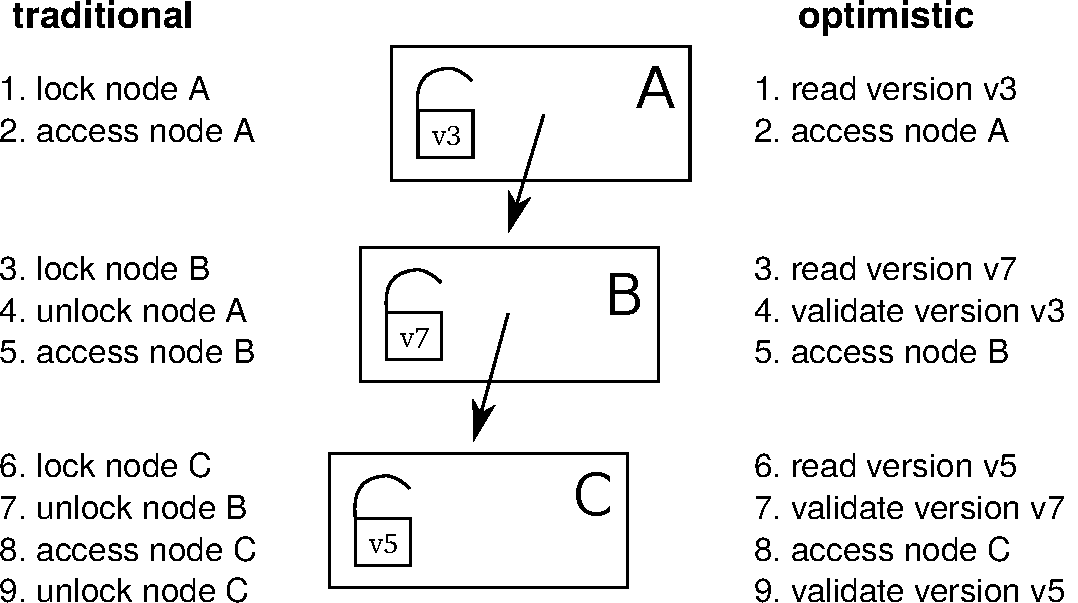
\includegraphics[width=0.65\linewidth]{olcall.pdf}
  \vspace{0.2cm}
  \caption{Comparison of a lookup operation in a 3-level tree using traditional lock coupling (left-hand side) vs.~optimistic lock coupling (right-hand side).}
  \label{fig:olc}
\end{figure}

The traditional and most common lock-based synchronization protocol for B-trees is lock coupling, which interleaves lock acquisitions while holding at most two locks at a time.
If, as we observed earlier, optimistic locks have similar semantics as traditional locks, it is natural to ask whether lock coupling can be combined with optimistic locks.
And indeed the answer is yes: One can almost mechanically translate traditional lock coupling code to optimistic lock coupling code.
This is illustrated in Figure~\ref{fig:olc}, which compares the traversal in a tree of height 3 using traditional and optimistic locks.
As the figure shows, the main difference is that locking is translated to reading the version and that unlocking becomes validation of the previously read version.
This simple change provides efficient lock-free tree traversal without the need to design a complex synchronization protocol.

It is important to emphasize the conceptual simplicity of OLC in comparison to data structures that use custom protocols like the Bw-tree~\cite{DBLP:conf/icde/LevandoskiLS13a}.
To implement lock-free access, the Bw-tree requires an indirection table, delta nodes, complex splitting and merging logic, retry logic, etc.
OLC, on the other hand, can directly be applied to B-trees mostly by adding the appropriate optimistic locking code and without modifying the node layout itself.
Therefore, OpenBw-Tree, an open source implementation of the Bw-tree, requires an order of magnitude more code than a B-tree based on OLC\footnote{Both implementations are available on GitHub: \url{https://github.com/wangziqi2016/index-microbench}}.
Given how difficult it is to develop, validate, and debug lock-free code, simplicity is obviously a major advantage.

\subsection{Correctness Aspects}

\begin{figure}
  % \centering
  %[basicstyle=\normalsize\ttfamily,showstringspaces=false,columns=fullflexible,breaklines=false,breakatwhitespace=true,numbers=none,numberstyle=\small,style=C,keepspaces=true]
\begin{lstlisting}[basicstyle=\ttfamily,language=C++,numbers=left,numberstyle=\small]
std::atomic<BTreeNode*> root;

// search for key in B+tree, returns payload in resultOut
bool lookup(Key key, Value& resultOut) {
   BTreeNode* node = root.load();
   uint64_t nodeVersion = node->readLockOrRestart();
   if (node != root.load()) // make sure the root is still the root
      restart();

   BTreeInner<Key>* parent = nullptr;
   uint64_t parentVersion = 0;

   while (node->isInner()) {
      auto inner = (BTreeInner*)node;

      // unlock parent and make current node the parent
      if (parent)
         parent->readUnlockOrRestart(parentVersion);
      parent = inner;
      parentVersion = nodeVersion;

      // search for next node
      node = inner->findChild(key);
      // validate 'inner' to ensure that 'node' pointer is valid
      inner->checkOrRestart(nodeVersion);
      // now it safe to dereference 'node' pointer (read its version)
      nodeVersion = node->readLockOrRestart();
   }

   // search in leaf and retrieve payload
   auto leaf = (BTreeLeaf*)node;
   bool success = leaf->findValue(key, resultOut);

   // unlock everything
   if (parent)
      parent->readUnlockOrRestart(parentVersion);
   node->readUnlockOrRestart(nodeVersion);

   return success;
}
\end{lstlisting}
  \vspace{0.2cm}
  \caption{B-tree lookup code using OLC. For simplicity, the restart logic is not shown.}
  \label{fig:lookup}
\end{figure}

So far, we have introduced the high-level ideas behind OLC and have stressed its similarity to traditional lock coupling.
Let us now discuss some cases where the close similarity between lock coupling and OLC breaks down.
To make this more concrete, we show the B-tree lookup code in Figure~\ref{fig:lookup}.
In the code, \texttt{readLockOrRestart} reads the lock version and \texttt{readUnlockOrRestart} validates that the read was correct.

One issue with OLC is that any pointer speculatively read from a node may point to invalid memory (if that node is modified concurrently).
Dereferencing such a pointer (e.g., to read its optimistic lock), may cause a segmentation fault or undefined behavior.
In the code shown in Figure~\ref{fig:lookup}, this problem is prevented by the extra check in line 25, which ensures that the read from the node containing the pointer was correct.
Without this additional validation, the code would in line 27 dereference the pointer speculatively read in line 23.
Note that the implementation of \texttt{checkOrRestart} is actually identical to \texttt{readUnlockOrRestart}.
We chose to give it a different name to highlight the fact that this extra check would not be necessary with read/write locks.

Another potential issue with optimistic locks is code that does not terminate.
Code that speculatively accesses a node, like an intra-node binary search, should be written in a way such that it always terminates---even in the presence of concurrent writes.
Otherwise, the validation code that detects the concurrent write will never run.
The binary search of a B-tree, for example, needs to be written in such a way that each comparison makes progress.
For some data structures that do not require loops in the traversal code (like ART) termination is trivially true.

\subsection{Implementation Details}

% implementation, efficiency
To implement an optimistic lock, one can combine the lock and the version counter into a single 64-bit\footnote{Even after subtracting one bit for the lock status, a back-of-the-envelope calculation can show that 63 bits are large enough to never overflow in practice.} word~\cite{artsync}.
A typical read operation will therefore merely consist of reading this version counter atomically.
In C++11 this can be implemented using the \texttt{std::atomic} type.

On x86, atomic reads are cheap because of x86's strong memory order guarantees.
No memory fences are required for sequentially-consistent loads, which are translated (by both GCC and clang) into standard \texttt{MOV} instructions.
Hence, the only effect of \texttt{std::atomic} for loads is preventing instruction re-ordering.
This makes version access and validation cheap.
Acquiring and releasing an optimistic lock in exclusive mode has comparable cost to a traditional lock:
A fairly expensive sequentially-consistent store is needed for acquiring a lock, while a standard \texttt{MOV} suffices for releasing it.
A simple sinlock-based implementation of optimistic locks can be found in the appendix of an earlier paper~\cite{artsync}.

OLC code must be able to handle restarts since validation or lock upgrade can fail due to concurrent writers.
Restarts can easily be implemented by wrapping the data structure operation in a loop (for simplicity not shown in Figure~\ref{fig:lookup}).
Such a loop also enables limiting the number of optimistic retry operations and falling back to pessimistic locking in cases of very heavy contention.
The ability to fall back to traditional locking is a major advantage of OLC in terms of robustness over lock-free approaches, which do not have this option.

In addition to the optimistic shared mode and the exclusive mode, optimistic locks also support a ``shared pessimistic'' mode, which physically acquires the lock in shared mode (allowing multiple concurrent readers but no writers).
This mode is useful for table (or range) scans that touch many tuples on a leaf page (which would otherwise easily abort).
Finally, let us mention that large range scans and table scans, should be broken up into several per-node traversals as is done in the LeanStore~\cite{leanstore} system.

Like all lock-free data structures, but unlike traditional locking and Hardware Transactional Memory~\cite{DBLP:conf/hpca/KarnagelDRLLSL14,DBLP:journals/pvldb/MakreshanskiLS15,htmtkde}, OLC requires care when deleting (and reusing) nodes.
The reason is that a deleting thread can never be sure that a node can be reclaimed because other threads might still be optimistically reading from that node.
Therefore, standard solutions like epoch-based reclamation~\cite{DBLP:conf/sosp/TuZKLM13}, hazard pointers~\cite{DBLP:journals/tpds/Michael04}, or optimized hazard pointers~\cite{DBLP:conf/spaa/BalmauGHZ16} need to be used.
These memory reclamation techniques are, however, largely orthogonal to the synchronization protocol itself.

%-lock-free is not a strong guarantee

\newpage
\section{Evaluation}\label{sec:evaluation}

Let us now experimentally evaluate the overhead and scalability of OLC.
For the experiments, we use an in-memory B+tree implemented in C++11 using templates, which is configured to use nodes of 4096 bytes, random 8 byte keys, and 8 byte payloads.
Based on this B-tree, we compare the following synchronization approaches:
\begin{itemize}
\item an OLC implementation\footnote{An almost identical OLC implementation is available on github: \url{https://github.com/wangziqi2016/index-microbench/tree/master/BTreeOLC}}
\item a variant based on traditional lock coupling and read/write locks
\item the unsynchronized B-tree, which obviously is only correct for read-only workloads but allows measuring the overhead of synchronization
\end{itemize}
Note that earlier work has compared the OLC implementation with a Bw-tree implementation~\cite{buzzword} and other state-of-the-art in-memory index structures.

We use a Haswell EP system with an Intel Xeon E5-2687W v3 CPU, which has 10 cores (20 ``Hyper-Threads'') and 25~MB of L3 cache.
The system is running Ubuntu 18.10 and we use GCC 8.2.0 to compile our code.
The CPU counters are obtained using the Linux perf API\footnote{We use the following convenience wrapper: \url{https://github.com/viktorleis/perfevent}}.

\begin{table}
  \caption{Performance and CPU counters for lookup and insert operations in a B-tree with 100M keys. We perform 100M operations and normalize the CPU counters by that number.}
  \label{tab:overhead}
  \centering
  \begin{tabular}{lrrrrrrr}\toprule
                    &         &        &        & instruc-  & L1     & L3     & branch \\
                    & threads & M op/s & cycles & tions & misses & misses & misses \\\midrule
lookup (no sync.)   & 1       & 1.72   & 2028   & 283     & 39.1   & 14.9   & 16.1   \\
lookup (OLC)        & 1       & 1.65   & 2107   & 370     & 43.9   & 15.1   & 16.7   \\
lookup (lock coup.) & 1       & 1.72   & 2078   & 365     & 42.3   & 16.9   & 15.7   \\\midrule
insert (no sync.)   & 1       & 1.51   & 2286   & 530     & 59.8   & 31.1   & 17.3   \\
insert (OLC)        & 1       & 1.50   & 2303   & 629     & 61.2   & 31.1   & 16.5   \\
insert (lock coup.) & 1       & 1.41   & 2473   & 644     & 61.0   & 31.0   & 17.2   \\\midrule
lookup (no sync.)   & 10      & 15.48  & 2058   & 283     & 38.6   & 15.5   & 16.0   \\
lookup (OLC)        & 10      & 14.60  & 2187   & 370     & 43.8   & 15.8   & 16.8   \\
lookup (lock coup.) & 10      & 5.71   & 5591   & 379     & 54.2   & 17.0   & 14.8   \\\midrule
insert (no sync.)   & 10      & -      & -      & -       & -      & -      & -      \\
insert (OLC)        & 10      & 10.46  & 2940   & 656     & 62.0   & 32.5   & 16.8   \\
insert (lock coup.) & 10      & 7.55   & 4161   & 667     & 75.0   & 28.6   & 16.2   \\
    \bottomrule
\end{tabular}
\end{table}

Table~\ref{tab:overhead} compares the performance and CPU counters for lookup and insert operations in a B-tree with 100M keys.
With {\em single-threaded} execution, we observe that all three approaches have very similar performance.
Adding traditional or optimistic locks to unsynchronized B-tree code results in up to 30\% of additional instructions without affecting single-threaded performance much.

\begin{figure}
  \centering
  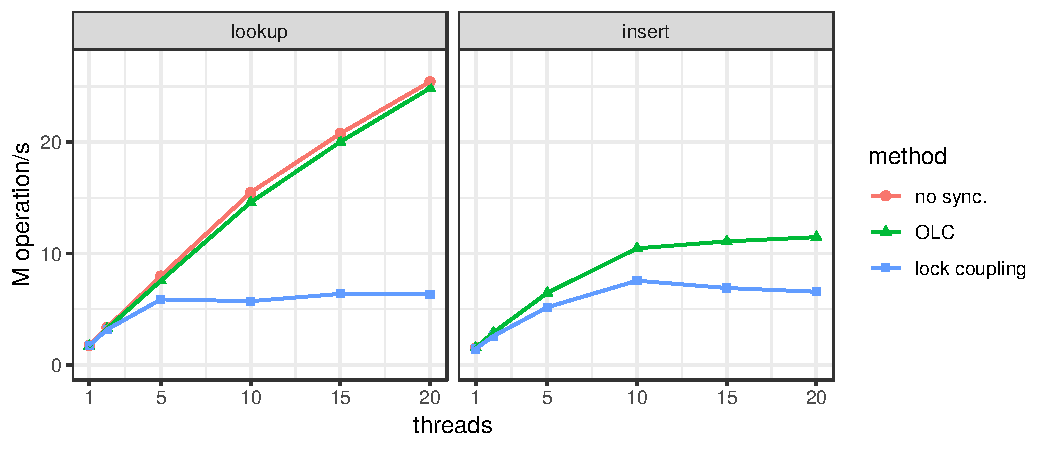
\includegraphics[width=\linewidth]{scale.pdf}
  \vspace{0.2cm}
  \caption{Scalability on 10-core system for B-tree operations (100M values).}
  \label{fig:scale}
\end{figure}

As Figure~\ref{fig:scale} shows, the results change dramatically once we use multiple threads.
For lookup, the scalability of OLC is near-linear up to 20 threads, even though the system has only 10 ``real cores''.
The OLC scalability for insert is also respectable (though not quite as linear because multi-threaded insertion approaches the memory bandwidth of our processor).
The figure also shows that the results of traditional lock coupling with read/write locks are significantly worse than OLC.
With 20 threads, lookup with OLC is 3.9$\times$ faster than traditional lock coupling.

\section{Summary}\label{sec:conc}

Optimistic Lock Coupling (OLC) is an effective synchronization method that combines the simplicity of traditional lock coupling with the superior scalability of lock-free approaches.
OLC is widely applicable and has already been successfully used to synchronize several data structures, including B-trees, binary search trees, and different trie variants.
These features make it highly attractive for modern database systems as well as performance-critical systems software in general.

\begin{thebibliography}{10}

\bibitem{DBLP:conf/spaa/BalmauGHZ16}
O.~Balmau, R.~Guerraoui, M.~Herlihy, and I.~Zablotchi.
\newblock Fast and robust memory reclamation for concurrent data structures.
\newblock In {\em SPAA}, 2016.

\bibitem{DBLP:journals/acta/BayerS77}
R.~Bayer and M.~Schkolnick.
\newblock Concurrency of operations on {B}-trees.
\newblock {\em Acta Informatica}, 9, 1977.

\bibitem{hot}
R.~Binna, E.~Zangerle, M.~Pichl, G.~Specht, and V.~Leis.
\newblock {HOT}: A height optimized trie index for main-memory database
  systems.
\newblock In {\em SIGMOD}, 2018.

\bibitem{DBLP:conf/ppopp/BronsonCCO10}
N.~G. Bronson, J.~Casper, H.~Chafi, and K.~Olukotun.
\newblock A practical concurrent binary search tree.
\newblock In {\em PPOPP}, 2010.

\bibitem{DBLP:conf/vldb/ChaHKK01}
S.~K. Cha, S.~Hwang, K.~Kim, and K.~Kwon.
\newblock Cache-conscious concurrency control of main-memory indexes on
  shared-memory multiprocessor systems.
\newblock In {\em VLDB}, 2001.

\bibitem{intel}
I.~Cutress.
\newblock {Intel} goes for 48-cores: {Cascade-AP} with multi-chip package
  coming soon.
\newblock
  \url{https://www.anandtech.com/show/13535/intel-goes-for-48cores-cascade-ap},
  2018 (accessed January, 2019).

\bibitem{DBLP:conf/cidr/FaleiroA17}
J.~M. Faleiro and D.~J. Abadi.
\newblock Latch-free synchronization in database systems: Silver bullet or
  fool's gold?
\newblock In {\em CIDR}, 2017.

\bibitem{DBLP:journals/ftdb/Graefe11}
G.~Graefe.
\newblock Modern {B}-tree techniques.
\newblock {\em Foundations and Trends in Databases}, 3(4), 2011.

\bibitem{DBLP:conf/hpca/KarnagelDRLLSL14}
T.~Karnagel, R.~Dementiev, R.~Rajwar, K.~Lai, T.~Legler, B.~Schlegel, and
  W.~Lehner.
\newblock Improving in-memory database index performance with
  {Intel}\({}^{\mbox{{\textregistered}}}\) transactional synchronization
  extensions.
\newblock In {\em HPCA}, 2014.

\bibitem{DBLP:journals/tods/LehmanY81}
P.~L. Lehman and S.~B. Yao.
\newblock Efficient locking for concurrent operations on {B}-trees.
\newblock {\em {ACM} Trans. Database Syst.}, 6(4), 1981.

\bibitem{leanstore}
V.~Leis, M.~Haubenschild, A.~Kemper, and T.~Neumann.
\newblock Leanstore: In-memory data management beyond main memory.
\newblock In {\em ICDE}, 2018.

\bibitem{art}
V.~Leis, A.~Kemper, and T.~Neumann.
\newblock The adaptive radix tree: {ARTful} indexing for main-memory databases.
\newblock In {\em ICDE}, 2013.

\bibitem{htmtkde}
V.~Leis, A.~Kemper, and T.~Neumann.
\newblock Scaling {HTM}-supported database transactions to many cores.
\newblock {\em {IEEE} Trans. Knowl. Data Eng.}, 28(2), 2016.

\bibitem{artsync}
V.~Leis, F.~Scheibner, A.~Kemper, and T.~Neumann.
\newblock The {ART} of practical synchronization.
\newblock In {\em DaMoN}, 2016.

\bibitem{DBLP:conf/icde/LevandoskiLS13a}
J.~J. Levandoski, D.~B. Lomet, and S.~Sengupta.
\newblock The {Bw}-tree: A {B}-tree for new hardware platforms.
\newblock In {\em ICDE}, 2013.

\bibitem{DBLP:journals/pvldb/MakreshanskiLS15}
D.~Makreshanski, J.~J. Levandoski, and R.~Stutsman.
\newblock To lock, swap, or elide: On the interplay of hardware transactional
  memory and lock-free indexing.
\newblock {\em {PVLDB}}, 8(11), 2015.

\bibitem{DBLP:dblp_conf/eurosys/MaoKM12}
Y.~Mao, E.~Kohler, and R.~T. Morris.
\newblock Cache craftiness for fast multicore key-value storage.
\newblock In {\em EuroSys}, 2012.

\bibitem{DBLP:journals/tpds/Michael04}
M.~M. Michael.
\newblock Hazard pointers: Safe memory reclamation for lock-free objects.
\newblock {\em {IEEE} Trans. Parallel Distrib. Syst.}, 15(6), 2004.

\bibitem{DBLP:journals/jacm/ShalevS06}
O.~Shalev and N.~Shavit.
\newblock Split-ordered lists: Lock-free extensible hash tables.
\newblock {\em J. {ACM}}, 53(3), 2006.

\bibitem{amd}
A.~Shilov.
\newblock {AMD} previews {EPYC} ‘{Rome}’ processor: Up to 64 {Zen} 2 cores.
\newblock
  \url{https://www.anandtech.com/show/13561/amd-previews-epyc-rome-processor-up-to-64-zen-2-cores},
  2018 (accessed January, 2019).

\bibitem{DBLP:conf/sosp/TuZKLM13}
S.~Tu, W.~Zheng, E.~Kohler, B.~Liskov, and S.~Madden.
\newblock Speedy transactions in multicore in-memory databases.
\newblock In {\em SOSP}, 2013.

\bibitem{buzzword}
Z.~Wang, A.~Pavlo, H.~Lim, V.~Leis, H.~Zhang, M.~Kaminsky, and D.~Andersen.
\newblock Building a {Bw}-tree takes more than just buzz words.
\newblock In {\em SIGMOD}, 2018.

\end{thebibliography}


%\bibliographystyle{abbrv}
%\bibliography{main}

\end{document}

\end{article}
\begin{article}
{Transparent Decisions: Selective Information Disclosure To Generate Synthetic Data}
{Carlos Gavidia-Calderon, Steve Harris, Markus Hauru, Florimond Houssiau,
Carsten Maple, Iain Stenson, May Yong}
\pdfminorversion=5
\documentclass[11pt]{article}
\usepackage{deauthor,times,graphicx,caption,microtype}
\usepackage{hyperref}
\usepackage{listings}
\usepackage{booktabs}

\begin{document}

\title{Optimistic Lock Coupling: A Scalable and Efficient General-Purpose Synchronization Method}

\author{Viktor Leis, Michael Haubenschild\raisebox{0.9ex}{$\ast$}, Thomas Neumann\\ Technische Universit{\"a}t M{\"u}nchen \hspace{0.7cm} Tableau Software\raisebox{0.9ex}{$\ast$} \\ {\{leis,neumann\}{@}in.tum.de} \hspace{0.7cm} {mhaubenschild{@}tableau.com\raisebox{0.9ex}{$\ast$}}}

\maketitle

\begin{abstract}
As the number of cores on commodity processors continues to increase, scalability becomes more and more crucial for overall performance.
Scalable and efficient concurrent data structures are particularly important, as these are often the building blocks of parallel algorithms.
Unfortunately, traditional synchronization techniques based on fine-grained locking have been shown to be unscalable on modern multi-core CPUs.
Lock-free data structures, on the other hand, are extremely difficult to design and often incur significant overhead.

In this work, we make the case for Optimistic Lock Coupling as a practical alternative to both traditional locking and the lock-free approach.
We show that Optimistic Lock Coupling is highly scalable and almost as simple to implement as traditional lock coupling.
Another important advantage is that it is easily applicable to most tree-like data structures.
We therefore argue that Optimistic Lock Coupling, rather than a complex and error-prone custom synchronization protocol, should be the default choice for performance-critical data structures.
\end{abstract}

\section{Introduction}

% more and more cores
Today, Intel's commodity server processors have up to 28 cores and its upcoming microarchitecture will have up to 48 cores per socket~\cite{intel}.
Similarly, AMD currently stands at 32 cores and this number is expected to double in the next generation~\cite{amd}.
Since both platforms support simultaneous multithreading (also known as hyperthreading), affordable commodity servers (with up to two sockets) will soon routinely have between 100 and 200 hardware threads.

% data structure scalability is important
With such a high degree of hardware parallelism, efficient data processing crucially depends on how well concurrent data structures scale.
Internally, database systems use a plethora of data structures like table heaps, internal work queues, and, most importantly, index structures.
Any of these can easily become a scalability (and therefore overall performance) bottleneck on many-core CPUs.

% traditional synchronization: fine-grained locks, slow, cache invalidation
Traditionally, database systems synchronize internal data structures using fine-grained reader/writer locks\footnote{In this work, we focus on data structure synchronization rather than high-level transaction semantics and therefore use the term {\em lock} for what would typically be called {\em latch} in the database literature. We thus follow common computer science (rather than database) terminology.}.
Unfortunately, while fine-grained locking makes lock contention unlikely, it still results in bad scalability because lock acquisition and release require writing to shared memory.
Due to the way cache coherency is implemented on modern multi-core CPUs, these writes cause additional cache misses\footnote{The cache coherency protocol ensures that all copies of a cache line on other cores are invalidated before the write can proceed.} and the cache line containing the lock's internal data becomes a point of physical contention.
As a result, any frequently-accessed lock (e.g., the lock of the root node of a B-tree) severely limits scalability.

% lock-free bw-tree: no more latches, but indirections, extremely complex
Lock-free data structures like the Bw-tree~\cite{DBLP:conf/icde/LevandoskiLS13a} (a lock-free B-tree variant) or the Split-Ordered List~\cite{DBLP:journals/jacm/ShalevS06} (a lock-free hash table) do not acquire any locks and therefore generally scale much better than locking-based approaches (in particular for read-mostly workloads).
However, lock-free synchronization has other downsides:
First, it is very difficult and results in extremely complex and error-prone code (when compared to locking).
Second, because the functionality of atomic primitives provided by the hardware (e.g., atomically compare-and-swap 8 bytes) is limited, complex operations require additional indirections within the data structure.
For example, the Bw-tree requires an indirection table and the Split-Ordered List requires ``dummy nodes'', resulting in overhead due to additional cache misses.

% OLC for the win
In this paper we make the case for {\em Optimistic Lock Coupling (OLC)}, a synchronization method that combines some of the best properties of lock-based and lock-free synchronization.
OLC utilizes a special lock type that can be used in two modes:
The first mode is similar to a traditional mutex and excludes other threads by physically acquiring the underlying lock.
In the second mode, reads can proceed optimistically by validating a version counter that is embedded in the lock (similar to optimistic concurrency control).
The first mode is typically used by writers and the second mode by readers.
Besides this special lock type, OLC is based on the observation that optimistic lock validations can be interleaved/coupled---similar to the pair-wise interleaved lock acquisition of traditional lock coupling.
Hence, the name Optimistic Lock Coupling.

OLC has a number of desirable features:
\begin{itemize}
\item By reducing the number of writes to shared memory locations and thereby avoiding cache invalidations, it {\bf scales well} for most workloads.
\item In comparison to unsynchronized code, it requires few additional CPU instructions making it {\bf efficient}.
\item OLC is {\bf widely applicable} to different data structures. It has already been successfully used for synchronizing binary search trees~\cite{DBLP:conf/ppopp/BronsonCCO10}, tries~\cite{artsync}, trie/B-tree hybrids~\cite{DBLP:dblp_conf/eurosys/MaoKM12}, and B-trees~\cite{buzzword}.
\item In comparison to the lock-free paradigm, it is also {\bf easy to use} and requires few modifications to existing, single-threaded data structures.
\end{itemize}
Despite these positive features and its simplicity, OLC is not yet widely known.
The goal of this paper is therefore to popularize this simple idea and to make a case for it.
We argue that OLC deserves to be widely known.
It is a good default synchronization paradigm---more complex, data structure-specific protocols are seldom beneficial.

The rest of the paper is organized as follows.
Section~\ref{sec:related} discusses related work, tracing the history of OLC and its underlying ideas in the literature.
The core of the paper is Section~\ref{sec:olc}, which describes the ideas behind OLC and how it can be used to synchronize complex data structures.
In Section~\ref{sec:evaluation} we experimentally show that OLC has low overhead and scales well when used to synchronize an in-memory B-tree.
We summarize the paper in Section~\ref{sec:conc}.

\newpage
\section{Related Work}\label{sec:related}

Lock coupling has been proposed as a method for allowing concurrent operations on B-trees in 1977~\cite{DBLP:journals/acta/BayerS77}.
This traditional and still widely-used method, described in detail in Graefe's B-tree survey~\cite{DBLP:journals/ftdb/Graefe11}, is also called ``latch coupling'', ``hand-over-hand locking'', and ``crabbing''.
Because at most two locks are held at-a-time during tree traversal, this technique seemingly allows for a high degree of parallelism---in particular if read/write locks are used to enable inner nodes to be locked in shared mode.
However, as we show in Section~\ref{sec:evaluation}, on modern hardware lock acquisition (even in shared mode) results in suboptimal scalability.

An early alternative from 1981 is a B-tree variant called B-link tree~\cite{DBLP:journals/tods/LehmanY81}, which only holds a single lock at a time.
It is based on the observation that between the release of the parent lock and the acquisition of the child lock, the only ``dangerous'' thing that could have happened is the split of a child node (assuming one does not implement merge operations).
Thus, when a split happens, the key being searched might end up on a neighboring node to the right of the current child node.
A B-link tree traversal therefore detects this condition and, if needed, transparently proceeds to the neighboring node.
Releasing the parent lock early is highly beneficial when the child node needs to be fetched from disk.
For in-memory workloads, however, the B-link tree has the same scalability issues as lock coupling (it acquires just as many locks).

The next major advance, Optimistic Latch-Free Index Traversal (OLFIT)~\cite{DBLP:conf/vldb/ChaHKK01}, was proposed in 2001.
OLFIT introduced the idea of a combined lock/update counter, which we call {\em optimistic lock}. % , for lack of a better name,
Based on these per-node optimistic locks and the synchronization protocol of the B-link tree, OLFIT finally achieves good scalability on parallel processors.
The OLFIT protocol is fairly complex, as it requires both the non-trivial B-link protocol and optimistic locks.
Furthermore, like the B-link tree protocol, it does not support merging nodes, and is specific to B-trees (cannot easily be applied to other data structures).

In the following two decades, the growth of main-memory capacity led to much research into other data structures besides the venerable B-tree.
Particularly relevant for our discussion is Bronson et al.'s~\cite{DBLP:conf/ppopp/BronsonCCO10} concurrent binary search tree, which is based on optimistic version validation and has a sophisticated, data structure-specific synchronization protocol.
To the best of our knowledge, this 2010 paper is the first that, as part of its protocol, interleaves version validation across nodes---rather than validating each node separately like OLFIT.
In that paper, this idea is called ``hand-over-hand, optimistic validation'', while we prefer the term Optimistic Lock Coupling to highlight the close resemblance to traditional lock coupling.
Similarly, Mao et al.'s~\cite{DBLP:dblp_conf/eurosys/MaoKM12} Masstree (a concurrent hybrid trie/B-tree) is also based on the same ideas, but again uses them as part of a more complex protocol.

The Adaptive Radix Tree (ART)~\cite{art} is another recent in-memory data structure, which we proposed in 2013.
In contrast to the two data structures just mentioned, it was originally designed with single-threaded performance in mind without supporting concurrency.
To add support for concurrency, we initially started designing a custom protocol called Read-Optimized Write Exclusion (ROWEX)~\cite{artsync}, which turned out to be non-trivial and requires modifications of the underlying data structure\footnote{Note that ROWEX is already easier to apply to existing data structures than the lock-free approach. The difficulty depends on the data structure. Applying ROWEX is hard for B-trees with sorted keys and fairly easy for copy-on-write data structures like the Height Optimized Trie~\cite{hot}---with ART being somewhere in the middle.}.
However, fairly late in the project, we also realized, that OLC {\em alone} (rather than as part of a more complex protocol) is sufficient to synchronize ART.
No other changes to the data structure were necessary.
Both approaches were published and experimentally evaluated in a followup paper~\cite{artsync}, which shows that, despite its simplicity, OLC is efficient, scalable, and generally outperforms ROWEX.

Similar results were recently published regarding B-trees~\cite{buzzword}.
In this experimental study a simple OLC-based synchronization outperformed the Bw-tree~\cite{DBLP:conf/icde/LevandoskiLS13a}, a complex lock-free synchronization approach.
Another recent paper shows that for write-intensive workloads, locking often performs better than lock-free synchronization~\cite{DBLP:conf/cidr/FaleiroA17}.
These experiences indicate that OLC is a general-purpose synchronization paradigm and motivate the current paper.

%foster b-tree\cite{DBLP:journals/tods/GraefeKK12}
%Shasha theory~\cite{DBLP:journals/tods/ShashaG88}

\section{Optimistic Lock Coupling}\label{sec:olc}

% locks suck
The standard technique for inter-thread synchronization is mutual exclusion using fine-grained locks.
In a B-tree, for example, every node usually has its own associated lock, which is acquired before accessing that node.
The problem of locking on modern multi- and many-core processors is that lock acquisition and release require writing to the shared memory location that implements the lock.
This write causes exclusive ownership of the underlying cache line and invalidates copies of it on all other processor cores.
For hierarchical, tree-like data structures, the lock of the root node becomes a point of physical contention---even in read-only workloads and even when read/write locks are used.
Depending on the specific data structure, number of cores, cache coherency protocol implementation, cache topology, whether Non-Uniform Memory Access (NUMA) is used, locking can even result in multi-threaded performance that is worse than single-threaded execution.

% in b-trees this happens very much
The inherent pessimism of locking is particularly unfortunate for B-trees:
Despite the fact that logical modifications of the root node are very infrequent, every B-tree operation must lock the root node during tree traversal\footnote{To a lesser extent this obviously applies to all inner nodes, not just the root.}.
Even the vast majority of update operations (with the exception of splits and merges), only modify a single leaf node.
These observations indicate that a more optimistic approach, which does not require locking inner nodes, would be very beneficial for B-trees.

\subsection{Optimistic Locks}

% optimism to the rescue
As the name indicates, optimistic locks try to solve the scalability issues of traditional locks using an optimistic approach.
Instead of always physically acquiring locks, even for nodes that are unlikely to be modified simultaneously, after-the-fact validation is used to detect conflicts.
This is done by augmenting each lock with a version/update counter that is incremented on every modification.
Using this version counter, readers can optimistically proceed before validating that the version did not change to ensure that the read was safe.
If validation fails, the operation is restarted.

% details on opt locks
Using optimistic locks, a read-only node access (i.e., the majority of all operations in a B-tree) does not acquire the lock and does not increment the version counter.
Instead, it performs the following steps:
\begin{enumerate}
\item read lock version (restart if lock is not free)
\item access node
\item read the version again and validate that it has not changed in the meantime
\end{enumerate}
If the last step (the validation) fails, the operation has to be restarted.
Write operations, on the other hand, are more similar to traditional locking:
\begin{enumerate}
\item acquire lock (wait if necessary)
\item access/write to node
\item increment version and unlock node
\end{enumerate}
Writes can therefore protect a node from other writes.

% similar to locks
As we observed in an earlier paper~\cite{artsync}, because of similar semantics, optimistic locks can be hidden behind an API very similar to traditional read/write locks.
Both approaches have an exclusive lock mode, and acquiring a traditional lock in shared mode is analogous to optimistic version validation.
Furthermore, like with some implementations of traditional read/write locks, optimistic locks allow upgrading a shared lock to an exclusive lock.
Lock upgrades are, for example, used to avoid most B-tree update operations from having to lock inner nodes.
In our experience, the close resemblance of optimistic and traditional locks simplifies the reasoning about optimistic locks;
one can apply similar thinking as in traditional lock-based protocols.

\subsection{Lock Coupling with Optimistic Locks}

\begin{figure}
  \centering
  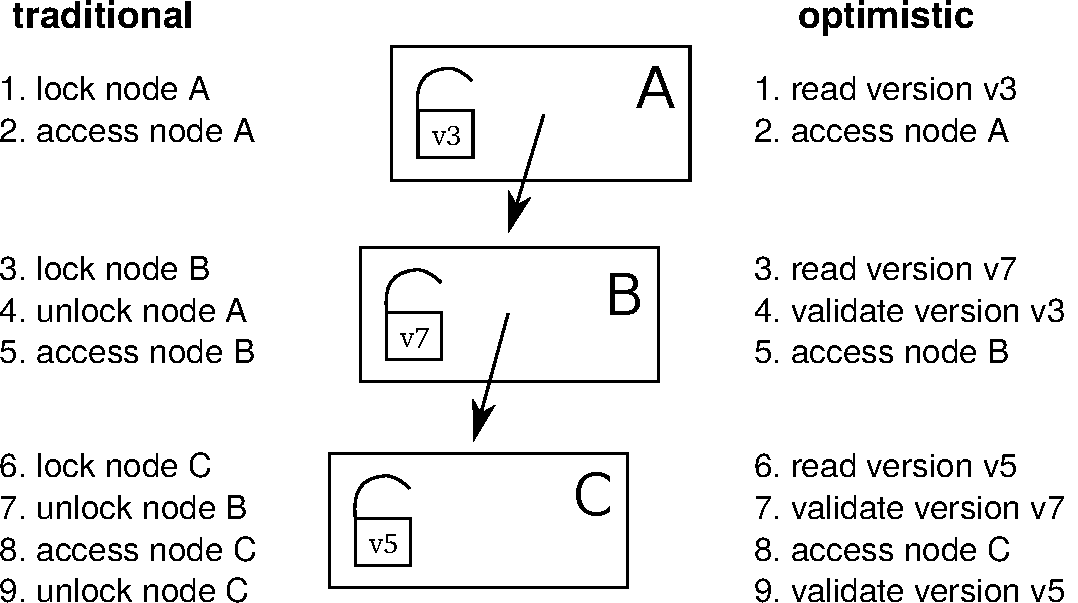
\includegraphics[width=0.65\linewidth]{olcall.pdf}
  \vspace{0.2cm}
  \caption{Comparison of a lookup operation in a 3-level tree using traditional lock coupling (left-hand side) vs.~optimistic lock coupling (right-hand side).}
  \label{fig:olc}
\end{figure}

The traditional and most common lock-based synchronization protocol for B-trees is lock coupling, which interleaves lock acquisitions while holding at most two locks at a time.
If, as we observed earlier, optimistic locks have similar semantics as traditional locks, it is natural to ask whether lock coupling can be combined with optimistic locks.
And indeed the answer is yes: One can almost mechanically translate traditional lock coupling code to optimistic lock coupling code.
This is illustrated in Figure~\ref{fig:olc}, which compares the traversal in a tree of height 3 using traditional and optimistic locks.
As the figure shows, the main difference is that locking is translated to reading the version and that unlocking becomes validation of the previously read version.
This simple change provides efficient lock-free tree traversal without the need to design a complex synchronization protocol.

It is important to emphasize the conceptual simplicity of OLC in comparison to data structures that use custom protocols like the Bw-tree~\cite{DBLP:conf/icde/LevandoskiLS13a}.
To implement lock-free access, the Bw-tree requires an indirection table, delta nodes, complex splitting and merging logic, retry logic, etc.
OLC, on the other hand, can directly be applied to B-trees mostly by adding the appropriate optimistic locking code and without modifying the node layout itself.
Therefore, OpenBw-Tree, an open source implementation of the Bw-tree, requires an order of magnitude more code than a B-tree based on OLC\footnote{Both implementations are available on GitHub: \url{https://github.com/wangziqi2016/index-microbench}}.
Given how difficult it is to develop, validate, and debug lock-free code, simplicity is obviously a major advantage.

\subsection{Correctness Aspects}

\begin{figure}
  % \centering
  %[basicstyle=\normalsize\ttfamily,showstringspaces=false,columns=fullflexible,breaklines=false,breakatwhitespace=true,numbers=none,numberstyle=\small,style=C,keepspaces=true]
\begin{lstlisting}[basicstyle=\ttfamily,language=C++,numbers=left,numberstyle=\small]
std::atomic<BTreeNode*> root;

// search for key in B+tree, returns payload in resultOut
bool lookup(Key key, Value& resultOut) {
   BTreeNode* node = root.load();
   uint64_t nodeVersion = node->readLockOrRestart();
   if (node != root.load()) // make sure the root is still the root
      restart();

   BTreeInner<Key>* parent = nullptr;
   uint64_t parentVersion = 0;

   while (node->isInner()) {
      auto inner = (BTreeInner*)node;

      // unlock parent and make current node the parent
      if (parent)
         parent->readUnlockOrRestart(parentVersion);
      parent = inner;
      parentVersion = nodeVersion;

      // search for next node
      node = inner->findChild(key);
      // validate 'inner' to ensure that 'node' pointer is valid
      inner->checkOrRestart(nodeVersion);
      // now it safe to dereference 'node' pointer (read its version)
      nodeVersion = node->readLockOrRestart();
   }

   // search in leaf and retrieve payload
   auto leaf = (BTreeLeaf*)node;
   bool success = leaf->findValue(key, resultOut);

   // unlock everything
   if (parent)
      parent->readUnlockOrRestart(parentVersion);
   node->readUnlockOrRestart(nodeVersion);

   return success;
}
\end{lstlisting}
  \vspace{0.2cm}
  \caption{B-tree lookup code using OLC. For simplicity, the restart logic is not shown.}
  \label{fig:lookup}
\end{figure}

So far, we have introduced the high-level ideas behind OLC and have stressed its similarity to traditional lock coupling.
Let us now discuss some cases where the close similarity between lock coupling and OLC breaks down.
To make this more concrete, we show the B-tree lookup code in Figure~\ref{fig:lookup}.
In the code, \texttt{readLockOrRestart} reads the lock version and \texttt{readUnlockOrRestart} validates that the read was correct.

One issue with OLC is that any pointer speculatively read from a node may point to invalid memory (if that node is modified concurrently).
Dereferencing such a pointer (e.g., to read its optimistic lock), may cause a segmentation fault or undefined behavior.
In the code shown in Figure~\ref{fig:lookup}, this problem is prevented by the extra check in line 25, which ensures that the read from the node containing the pointer was correct.
Without this additional validation, the code would in line 27 dereference the pointer speculatively read in line 23.
Note that the implementation of \texttt{checkOrRestart} is actually identical to \texttt{readUnlockOrRestart}.
We chose to give it a different name to highlight the fact that this extra check would not be necessary with read/write locks.

Another potential issue with optimistic locks is code that does not terminate.
Code that speculatively accesses a node, like an intra-node binary search, should be written in a way such that it always terminates---even in the presence of concurrent writes.
Otherwise, the validation code that detects the concurrent write will never run.
The binary search of a B-tree, for example, needs to be written in such a way that each comparison makes progress.
For some data structures that do not require loops in the traversal code (like ART) termination is trivially true.

\subsection{Implementation Details}

% implementation, efficiency
To implement an optimistic lock, one can combine the lock and the version counter into a single 64-bit\footnote{Even after subtracting one bit for the lock status, a back-of-the-envelope calculation can show that 63 bits are large enough to never overflow in practice.} word~\cite{artsync}.
A typical read operation will therefore merely consist of reading this version counter atomically.
In C++11 this can be implemented using the \texttt{std::atomic} type.

On x86, atomic reads are cheap because of x86's strong memory order guarantees.
No memory fences are required for sequentially-consistent loads, which are translated (by both GCC and clang) into standard \texttt{MOV} instructions.
Hence, the only effect of \texttt{std::atomic} for loads is preventing instruction re-ordering.
This makes version access and validation cheap.
Acquiring and releasing an optimistic lock in exclusive mode has comparable cost to a traditional lock:
A fairly expensive sequentially-consistent store is needed for acquiring a lock, while a standard \texttt{MOV} suffices for releasing it.
A simple sinlock-based implementation of optimistic locks can be found in the appendix of an earlier paper~\cite{artsync}.

OLC code must be able to handle restarts since validation or lock upgrade can fail due to concurrent writers.
Restarts can easily be implemented by wrapping the data structure operation in a loop (for simplicity not shown in Figure~\ref{fig:lookup}).
Such a loop also enables limiting the number of optimistic retry operations and falling back to pessimistic locking in cases of very heavy contention.
The ability to fall back to traditional locking is a major advantage of OLC in terms of robustness over lock-free approaches, which do not have this option.

In addition to the optimistic shared mode and the exclusive mode, optimistic locks also support a ``shared pessimistic'' mode, which physically acquires the lock in shared mode (allowing multiple concurrent readers but no writers).
This mode is useful for table (or range) scans that touch many tuples on a leaf page (which would otherwise easily abort).
Finally, let us mention that large range scans and table scans, should be broken up into several per-node traversals as is done in the LeanStore~\cite{leanstore} system.

Like all lock-free data structures, but unlike traditional locking and Hardware Transactional Memory~\cite{DBLP:conf/hpca/KarnagelDRLLSL14,DBLP:journals/pvldb/MakreshanskiLS15,htmtkde}, OLC requires care when deleting (and reusing) nodes.
The reason is that a deleting thread can never be sure that a node can be reclaimed because other threads might still be optimistically reading from that node.
Therefore, standard solutions like epoch-based reclamation~\cite{DBLP:conf/sosp/TuZKLM13}, hazard pointers~\cite{DBLP:journals/tpds/Michael04}, or optimized hazard pointers~\cite{DBLP:conf/spaa/BalmauGHZ16} need to be used.
These memory reclamation techniques are, however, largely orthogonal to the synchronization protocol itself.

%-lock-free is not a strong guarantee

\newpage
\section{Evaluation}\label{sec:evaluation}

Let us now experimentally evaluate the overhead and scalability of OLC.
For the experiments, we use an in-memory B+tree implemented in C++11 using templates, which is configured to use nodes of 4096 bytes, random 8 byte keys, and 8 byte payloads.
Based on this B-tree, we compare the following synchronization approaches:
\begin{itemize}
\item an OLC implementation\footnote{An almost identical OLC implementation is available on github: \url{https://github.com/wangziqi2016/index-microbench/tree/master/BTreeOLC}}
\item a variant based on traditional lock coupling and read/write locks
\item the unsynchronized B-tree, which obviously is only correct for read-only workloads but allows measuring the overhead of synchronization
\end{itemize}
Note that earlier work has compared the OLC implementation with a Bw-tree implementation~\cite{buzzword} and other state-of-the-art in-memory index structures.

We use a Haswell EP system with an Intel Xeon E5-2687W v3 CPU, which has 10 cores (20 ``Hyper-Threads'') and 25~MB of L3 cache.
The system is running Ubuntu 18.10 and we use GCC 8.2.0 to compile our code.
The CPU counters are obtained using the Linux perf API\footnote{We use the following convenience wrapper: \url{https://github.com/viktorleis/perfevent}}.

\begin{table}
  \caption{Performance and CPU counters for lookup and insert operations in a B-tree with 100M keys. We perform 100M operations and normalize the CPU counters by that number.}
  \label{tab:overhead}
  \centering
  \begin{tabular}{lrrrrrrr}\toprule
                    &         &        &        & instruc-  & L1     & L3     & branch \\
                    & threads & M op/s & cycles & tions & misses & misses & misses \\\midrule
lookup (no sync.)   & 1       & 1.72   & 2028   & 283     & 39.1   & 14.9   & 16.1   \\
lookup (OLC)        & 1       & 1.65   & 2107   & 370     & 43.9   & 15.1   & 16.7   \\
lookup (lock coup.) & 1       & 1.72   & 2078   & 365     & 42.3   & 16.9   & 15.7   \\\midrule
insert (no sync.)   & 1       & 1.51   & 2286   & 530     & 59.8   & 31.1   & 17.3   \\
insert (OLC)        & 1       & 1.50   & 2303   & 629     & 61.2   & 31.1   & 16.5   \\
insert (lock coup.) & 1       & 1.41   & 2473   & 644     & 61.0   & 31.0   & 17.2   \\\midrule
lookup (no sync.)   & 10      & 15.48  & 2058   & 283     & 38.6   & 15.5   & 16.0   \\
lookup (OLC)        & 10      & 14.60  & 2187   & 370     & 43.8   & 15.8   & 16.8   \\
lookup (lock coup.) & 10      & 5.71   & 5591   & 379     & 54.2   & 17.0   & 14.8   \\\midrule
insert (no sync.)   & 10      & -      & -      & -       & -      & -      & -      \\
insert (OLC)        & 10      & 10.46  & 2940   & 656     & 62.0   & 32.5   & 16.8   \\
insert (lock coup.) & 10      & 7.55   & 4161   & 667     & 75.0   & 28.6   & 16.2   \\
    \bottomrule
\end{tabular}
\end{table}

Table~\ref{tab:overhead} compares the performance and CPU counters for lookup and insert operations in a B-tree with 100M keys.
With {\em single-threaded} execution, we observe that all three approaches have very similar performance.
Adding traditional or optimistic locks to unsynchronized B-tree code results in up to 30\% of additional instructions without affecting single-threaded performance much.

\begin{figure}
  \centering
  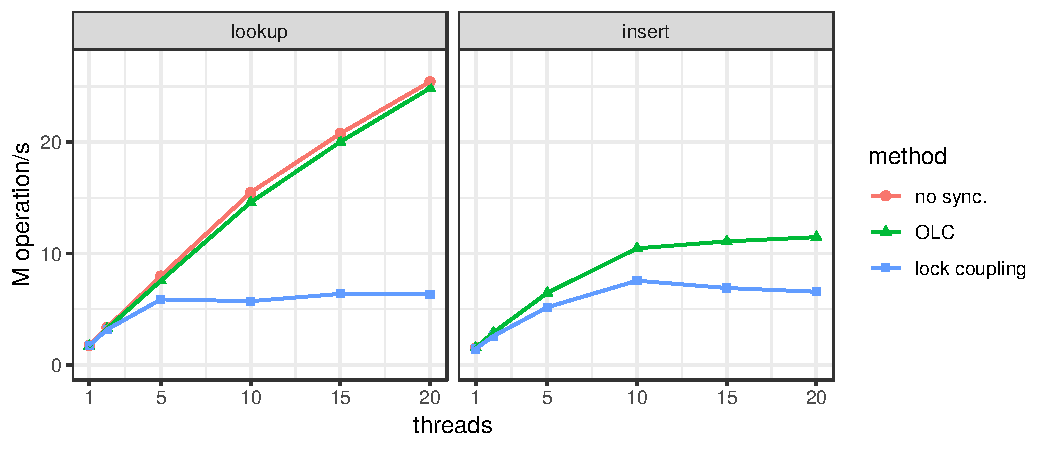
\includegraphics[width=\linewidth]{scale.pdf}
  \vspace{0.2cm}
  \caption{Scalability on 10-core system for B-tree operations (100M values).}
  \label{fig:scale}
\end{figure}

As Figure~\ref{fig:scale} shows, the results change dramatically once we use multiple threads.
For lookup, the scalability of OLC is near-linear up to 20 threads, even though the system has only 10 ``real cores''.
The OLC scalability for insert is also respectable (though not quite as linear because multi-threaded insertion approaches the memory bandwidth of our processor).
The figure also shows that the results of traditional lock coupling with read/write locks are significantly worse than OLC.
With 20 threads, lookup with OLC is 3.9$\times$ faster than traditional lock coupling.

\section{Summary}\label{sec:conc}

Optimistic Lock Coupling (OLC) is an effective synchronization method that combines the simplicity of traditional lock coupling with the superior scalability of lock-free approaches.
OLC is widely applicable and has already been successfully used to synchronize several data structures, including B-trees, binary search trees, and different trie variants.
These features make it highly attractive for modern database systems as well as performance-critical systems software in general.

\begin{thebibliography}{10}

\bibitem{DBLP:conf/spaa/BalmauGHZ16}
O.~Balmau, R.~Guerraoui, M.~Herlihy, and I.~Zablotchi.
\newblock Fast and robust memory reclamation for concurrent data structures.
\newblock In {\em SPAA}, 2016.

\bibitem{DBLP:journals/acta/BayerS77}
R.~Bayer and M.~Schkolnick.
\newblock Concurrency of operations on {B}-trees.
\newblock {\em Acta Informatica}, 9, 1977.

\bibitem{hot}
R.~Binna, E.~Zangerle, M.~Pichl, G.~Specht, and V.~Leis.
\newblock {HOT}: A height optimized trie index for main-memory database
  systems.
\newblock In {\em SIGMOD}, 2018.

\bibitem{DBLP:conf/ppopp/BronsonCCO10}
N.~G. Bronson, J.~Casper, H.~Chafi, and K.~Olukotun.
\newblock A practical concurrent binary search tree.
\newblock In {\em PPOPP}, 2010.

\bibitem{DBLP:conf/vldb/ChaHKK01}
S.~K. Cha, S.~Hwang, K.~Kim, and K.~Kwon.
\newblock Cache-conscious concurrency control of main-memory indexes on
  shared-memory multiprocessor systems.
\newblock In {\em VLDB}, 2001.

\bibitem{intel}
I.~Cutress.
\newblock {Intel} goes for 48-cores: {Cascade-AP} with multi-chip package
  coming soon.
\newblock
  \url{https://www.anandtech.com/show/13535/intel-goes-for-48cores-cascade-ap},
  2018 (accessed January, 2019).

\bibitem{DBLP:conf/cidr/FaleiroA17}
J.~M. Faleiro and D.~J. Abadi.
\newblock Latch-free synchronization in database systems: Silver bullet or
  fool's gold?
\newblock In {\em CIDR}, 2017.

\bibitem{DBLP:journals/ftdb/Graefe11}
G.~Graefe.
\newblock Modern {B}-tree techniques.
\newblock {\em Foundations and Trends in Databases}, 3(4), 2011.

\bibitem{DBLP:conf/hpca/KarnagelDRLLSL14}
T.~Karnagel, R.~Dementiev, R.~Rajwar, K.~Lai, T.~Legler, B.~Schlegel, and
  W.~Lehner.
\newblock Improving in-memory database index performance with
  {Intel}\({}^{\mbox{{\textregistered}}}\) transactional synchronization
  extensions.
\newblock In {\em HPCA}, 2014.

\bibitem{DBLP:journals/tods/LehmanY81}
P.~L. Lehman and S.~B. Yao.
\newblock Efficient locking for concurrent operations on {B}-trees.
\newblock {\em {ACM} Trans. Database Syst.}, 6(4), 1981.

\bibitem{leanstore}
V.~Leis, M.~Haubenschild, A.~Kemper, and T.~Neumann.
\newblock Leanstore: In-memory data management beyond main memory.
\newblock In {\em ICDE}, 2018.

\bibitem{art}
V.~Leis, A.~Kemper, and T.~Neumann.
\newblock The adaptive radix tree: {ARTful} indexing for main-memory databases.
\newblock In {\em ICDE}, 2013.

\bibitem{htmtkde}
V.~Leis, A.~Kemper, and T.~Neumann.
\newblock Scaling {HTM}-supported database transactions to many cores.
\newblock {\em {IEEE} Trans. Knowl. Data Eng.}, 28(2), 2016.

\bibitem{artsync}
V.~Leis, F.~Scheibner, A.~Kemper, and T.~Neumann.
\newblock The {ART} of practical synchronization.
\newblock In {\em DaMoN}, 2016.

\bibitem{DBLP:conf/icde/LevandoskiLS13a}
J.~J. Levandoski, D.~B. Lomet, and S.~Sengupta.
\newblock The {Bw}-tree: A {B}-tree for new hardware platforms.
\newblock In {\em ICDE}, 2013.

\bibitem{DBLP:journals/pvldb/MakreshanskiLS15}
D.~Makreshanski, J.~J. Levandoski, and R.~Stutsman.
\newblock To lock, swap, or elide: On the interplay of hardware transactional
  memory and lock-free indexing.
\newblock {\em {PVLDB}}, 8(11), 2015.

\bibitem{DBLP:dblp_conf/eurosys/MaoKM12}
Y.~Mao, E.~Kohler, and R.~T. Morris.
\newblock Cache craftiness for fast multicore key-value storage.
\newblock In {\em EuroSys}, 2012.

\bibitem{DBLP:journals/tpds/Michael04}
M.~M. Michael.
\newblock Hazard pointers: Safe memory reclamation for lock-free objects.
\newblock {\em {IEEE} Trans. Parallel Distrib. Syst.}, 15(6), 2004.

\bibitem{DBLP:journals/jacm/ShalevS06}
O.~Shalev and N.~Shavit.
\newblock Split-ordered lists: Lock-free extensible hash tables.
\newblock {\em J. {ACM}}, 53(3), 2006.

\bibitem{amd}
A.~Shilov.
\newblock {AMD} previews {EPYC} ‘{Rome}’ processor: Up to 64 {Zen} 2 cores.
\newblock
  \url{https://www.anandtech.com/show/13561/amd-previews-epyc-rome-processor-up-to-64-zen-2-cores},
  2018 (accessed January, 2019).

\bibitem{DBLP:conf/sosp/TuZKLM13}
S.~Tu, W.~Zheng, E.~Kohler, B.~Liskov, and S.~Madden.
\newblock Speedy transactions in multicore in-memory databases.
\newblock In {\em SOSP}, 2013.

\bibitem{buzzword}
Z.~Wang, A.~Pavlo, H.~Lim, V.~Leis, H.~Zhang, M.~Kaminsky, and D.~Andersen.
\newblock Building a {Bw}-tree takes more than just buzz words.
\newblock In {\em SIGMOD}, 2018.

\end{thebibliography}


%\bibliographystyle{abbrv}
%\bibliography{main}

\end{document}

\end{article}
\begin{article}
{Differential Privacy for Time Series: A Survey}
{Yulian Mao, Qingqing Ye, Qi Wang, Haibo Hu}
\documentclass[11pt,dvipdfm]{article}

\usepackage{deauthor,times,graphicx}
% \usepackage[a4paper, total={6.7in, 9.7in}]{geometry}

% JobGraph fig
\usepackage{tikz}
\usetikzlibrary{arrows,automata,positioning,shapes.geometric}

% trademark symbol
\usepackage{textcomp}

\usepackage{float}

% code listings
\usepackage{listings}

%\graphicspath{{submissions/submission4/figs/}}

\newcommand{\TODO}[1]{\textcolor{red}{TODO: #1}}
\newcommand{\sectionautorefname}{Section}%
\newcommand{\para}[1]{\vspace{2mm}\noindent\textbf{#1}}

\definecolor{dkgreen}{rgb}{0,0.6,0}
\definecolor{gray}{rgb}{0.5,0.5,0.5}
\definecolor{mauve}{rgb}{0.58,0,0.82}

% there is no built in support or Scala yet, good enough
\lstset{frame=l,
	language=Java,
	aboveskip=3mm,
	belowskip=3mm,
	showstringspaces=false,
	xleftmargin=5pt,
	%   framexleftmargin=-1pt,
	columns=flexible,
	basicstyle={\scriptsize\ttfamily},
	numbers=none,
	numberstyle=\tiny\color{black},
	keywordstyle=\color{blue},
	commentstyle=\color{dkgreen},
	stringstyle=\color{mauve},
	breaklines=true,
	breakatwhitespace=true,
	tabsize=4,
	%for scala
	emph={%
		object, def, val, zip, window, trigger, evict%
	},emphstyle={\color{blue}\textbf}%
}%


% \usepackage[
% % backend=biber
% % style=alphabetic,
% % sorting=abbrv
% ]{biblatex}

% \renewbibmacro{in:}{}


% \addbibresource{references.bib}
% \renewcommand{\bibfont}{\small} % or any other  appropriate font command

% url references
\usepackage{hyperref}

% in paragraph enums
\usepackage{paralist}

\def\definitionautorefname{Definition}
\def\sectionautorefname{Section}
\def\subsectionautorefname{Section}
\def\subsubsectionautorefname{Section}
\def\algorithmautorefname{Algorithm}
\def\figureautorefname{Figure}

\usepackage{amsmath}
\usepackage{amsfonts}
\usepackage{booktabs}
\usepackage{amssymb}
\usepackage{dsfont}

\usepackage{multirow}

\usepackage{tablefootnote}

\usepackage{natbib}

\usepackage{lipsum}

\newcommand\blfootnote[1]{%
	\begingroup
	\renewcommand\thefootnote{}\footnote{#1}%
	\addtocounter{footnote}{-1}%
	\endgroup
}



\begin{document}

% Use the commands below, not some other ones.

\title{Task-Focused Information Retrieval in the Generative AI Era}

\author{Chirag Shah\textsuperscript{1} and Ryen W. White\textsuperscript{2}\\
	\textsuperscript{1}\small{University of Washington, Seattle, WA, USA}\\
	\textsuperscript{2}\small{Microsoft Research, Redmond, WA, USA}\\
	\small{chirags@uw.edu, ryenw@microsoft.com}
}

\maketitle

\begin{abstract}
Generative Artificial Intelligence (GenAI) is revolutionizing how people access information and how they tackle and complete complex information tasks. This report is a summary of a recent workshop at Microsoft on this important and pressing topic. The event brought together a diverse mix of attendees from different professions and at different career stages for an engaging day of presentations and  discussions. The emergent themes are described in detail in this summary. 
\end{abstract}

% Body of paper.  The paper should be present as a single file.
% Do not include other files for sections of the paper.
% Papers should not be longer than 12 pages

% ALL FIGURES MUST BE IN A SUBFOLDER NAMED figs
% See fig-guide for advice about figures
% Your paper's pdf should be less than 500K bytes

% Figures should be include in your paper using
% the \includegraphics command


% YOUR PAPER GOES HERE

\section{Introduction}
The second workshop on ``Task-Focused Information Retrieval in the Generative AI Era" was held on September 27, 2024 on Microsoft campus in Redmond, Washington. Around 60 participants from various organizations -- academic and industry -- and various positions -- students, faculty, professionals -- from across the United States came together for this one day in discussing issues related to information retrieval and access systems in the context of GenAI, specifically GenAI tools such as Large Language Models (LLMs). More information on the workshop, including the agenda, is available at \url{https://ir-ai.github.io}.

At the beginning of the workshop, the participants were asked to come up with a set of specific questions or topics pertaining to the larger area of task-focused Information Retrieval (IR) systems in the context of GenAI. Dozens of questions, ideas, and topics were posted on a large whiteboard using sticky notes. Participants then arranged these notes into four broad categories: (1) theory, (2) benchmarks and evaluation, (3) users and user experience, and (4) applications and integration.

For the remainder of the day, we organized breakout sessions where the participants used the notes for the corresponding topics to stem their discussions and expand on their ideas. The groups took notes in a shared document. The following sections summarize the key points from their notes and the discussions.

\section{Theory}
While there were many threads of discussions on various theoretical constructs in GenAI, such as context, language, and interactions, the groups spent a significant amount of time talking about relearning (updating the model knowledge or capabilities based on new data or feedback), unlearning (removing knowledge learned during training, e.g., for privacy, copyright, etc.), and readjustments for LLMs when it comes to information access. This is particularly needed to address issues of privacy, bias, and toxicity while also providing a more flexible architecture for further learning and refinements. For example, the following approaches were discussed for unlearning in LLMs:

\begin{enumerate}
    \item {\bf Training the Foundational Model}: This approach was found to be not feasible in most situations due to the need to retrain the model for every data removal request.
    \item {\bf Decoding Strategies}: This will involve preventing generation of certain tokens. However, models might find alternative ways to express similar intents.
    \item {\bf Guardrails/Censorship}: This idea requires implementing a layer to discourage certain topics and training the LLM to provide more diplomatic answers instead of deleting information.
    \item {\bf Reinforcement Learning from Human Feedback (RLHF)}: This popular technique to align LLMs with human preferences \cite{ziegler2019fine} can be used after initial training to discourage specific concepts/tokens.
\end{enumerate}

Workshop participants also discussed alternative ways to train a foundational model for better, more flexible and nuanced training, e.g.,

\begin{enumerate}
    \item {\bf Speculative Decoding}: This approach is based on student-teacher concept with a small and large model where they decode tokens sequentially and a large model that verifies tokens as they go. This approach improves efficiency and has been found that it does not affect accuracy \cite{leviathan2023fast}.%The idea is to use an LLM that acts as a guardian.
    \item {\bf Segmented Corpuses}: This approach involves training different segments of a large corpus based on expertise for specific motives.
    \item {\bf Multi-agent Auditing}: Use experts to prevent other LLMs from generating unlearned content.
    \item {\bf Distributed Models vs. Single/Centralized Model}: Mimic the human neuron system for more efficient inference and storage.
    \item{\bf Graph/Network of Models}: Each node is responsible for a specific concept, requiring sufficient common ground for communication.
\end{enumerate}

\section{Benchmarks and Evaluation}
Two breakout groups focused on issues related to evaluation, datasets, and benchmarks for using GenAI for information access applications. The participants emphasized the importance of reliability and validity in evaluating and benchmarking LLMs. They noted that before establishing benchmarks, it is crucial to ensure both the benchmarks and the LLMs themselves are reliable and valid. This foundation is necessary to address issues of fairness, bias, and equity.

The groups highlighted the need for shared definitions of key terms and discussed how metrics should evolve to be more meaningful within specific tasks. Benchmarks should be context-specific to provide accurate evaluations.

When it comes to business use cases and {\bf personas}, the discussion focused on evaluating personalization effectiveness in relation to human preferences, laws, and values. The participants explored how to structure use cases, noting that product design often uses ``personas" to capture diverse user needs. However, it is challenging to cover all user differences with benchmarks, leading to questions about grouping users and assessing personalization without creating echo chambers or experiencing distribution collapse.

The groups also addressed the need for data to perform reliable evaluations. They discussed the scarcity of comprehensive {\bf open-source data} and suggested two solutions: using community data collection and encouraging organizations to release data collaboratively. Maintaining the quality of human evaluation was another key point. The participants emphasized the importance of context-specific questions to get accurate feedback.

On the topic of {\bf alignments and ethics}, they discussed aligning safety and ethical principles, evaluating alignment success, and maintaining privacy.

Finally, the groups touched on the concept of {\bf knowing}—specifically, how to get models to acknowledge when they do not know something. They suggested including confidence intervals in outputs and having models confirm or paraphrase inputs to improve transparency and reliability.

The discussion also covered the potential to teach LLMs appropriateness through system-level {\bf content moderation}, including parental controls, flags, and guardrails. They considered the importance of reading levels and the classification and generation of documents, noting that higher volumes of content could bypass filters.

Evaluating {\bf appropriateness} was another key topic. The group suggested using personalization algorithms to measure what is appropriate, understanding negative feedback, and utilizing both explicit and implicit user feedback to improve satisfaction. They also mentioned the importance of historical behavior logs and cultural evaluation and alignment, noting that standards change over time.

{\bf Context} was highlighted as crucial, with understanding intent being particularly challenging due to fuzzy boundaries and user subjectivity. The ability to solve complex queries and provide feedback interfaces for improvement was also discussed, along with fine-tuning for pluralistic alignment.

Finally, the group discussed setting contextual measures and measuring controllability, emphasizing the need for dynamic and temporal evaluation and the ability of LLMs to evaluate higher-level constructs.

\section{Users and User Experience}
In the breakout groups for discussing users and user experience, participants delved into the intricacies of enhancing user interaction and trust in LLMs. They began by emphasizing the importance of referring to ``people" instead of ``users" to better capture the human aspect of these interactions.

The conversation then shifted to the {\bf typology of tasks} that these people do, highlighting the need for systems that can effectively respond to various goals and intentions. For instance, assisting someone in learning how to apply for a green card requires a nuanced understanding of their needs, circumstances, and queries.

The usefulness of LLMs was discussed, with a focus on how it depends on both the individual and the system. Understanding the user involves considering the language used in queries, persona/user modeling, and cultural sensitivity. The group debated whether to curate pretraining data for users or to employ post-processing training methods.

Developing robust {\bf user simulators} emerged as a critical point, as current interaction patterns with LLMs are not well-defined. The challenge lies in creating a ``good enough" user simulator that accurately reflects real-world interactions.

Participants noted that while users may prefer simpler answers, which can increase the acceptance of LLMs, this preference can also lead to {\bf misinformation}. Balancing user engagement with well-being is crucial.

Extending the issue of misinformation, the discussion steered towards {\bf ethical considerations}. The group explored who controls the data, ownership, and access, questioning whether LLMs should always provide certifiable truths and discussing the broader social responsibilities of these models.

Building {\bf trust} was identified as fundamental. It is essential for LLMs to acknowledge when they do not know something. Using prompts to eliminate out-of-bound questions and effectively conveying uncertainty were highlighted as vital strategies for building trust.

The group also debated the necessity of pseudo-relevance feedback versus using LLMs to formulate queries. They explored whether a new form of {\bf relevance feedback}, more suited to the LLM era, is needed.

Designing systems that provide balanced perspectives and defining {\bf diversity} through user actions were key topics. The group discussed democratizing information access and involving user preferences before deploying models.

Understanding user behaviors and creating accurate {\bf user profiles} were emphasized. The discussion included improving existing user graphs (used to model and analyze connections between users, their activities, and the resources they interact with) and addressing privacy issues related to personalization.

{\bf Educating users} on how to interact effectively with LLMs was deemed crucial. The group debated the benefits of long description queries and how to capture diverse user preferences to ensure the system aligns with a broad user base.

{\bf Personalization} was recognized as having inherent risks, such as creating echo chambers. The group discussed whether the default mode should cater to general popular preferences or if users should be nudged with information from diverse contexts.

Addressing the {\bf cold start problem} and the influence of search systems/LLMs on query writing were also key points. The extent to which ideal queries should be dictated by the system was debated.

Throughout the discussion, references to foundational works, such as Robert S. Taylor's study on question negotiation \cite{taylor1968question} and information seeking in libraries, and Nicholas J. Belkin's concept of Anomalous States of Knowledge (ASK) \cite{belkin1980anomalous}, provided a theoretical backdrop.

Establishing trust and creating mechanisms to escape the pitfalls of personalization were emphasized as critical components for the future development of LLMs. The group concluded that ethical practices, user education, and robust evaluation methods are essential for enhancing the effectiveness and reliability of LLMs.

\section{Applications and Integration}
Finally, we had a breakout group for discussing multifaceted applications and integration of LLMs. They began by comparing the merits of general-purpose LLMs with those fine-tuned for specific tasks, weighing the benefits of versatility against the precision of specialization.

The conversation naturally flowed into the realm of {\bf multi-modal systems}, where information is conveyed through various formats such as text, images, and dynamic presentations. Participants debated the criteria for selecting these modalities, using examples like exploratory search, which might benefit from summaries, reference documents, and diverse outputs. They pondered whether LLMs should generate both text and images or focus solely on summarization, drawing parallels to Wikipedia's multi-modal approach.

The potential for LLMs to guide users along {\bf learning paths} was another key topic. Designing interactions that support dynamic search was emphasized, contrasting with traditional recommendation systems for movies and music, which can sometimes lead users into uninteresting rabbit holes. Unlike these systems, LLMs require carefully designed feedback mechanisms to ensure relevance and engagement. Learning, they noted, is not just about acquiring information on a specific topic; broader context and serendipity play crucial roles. Multi-modality was seen as particularly beneficial in applications such as claim verification, where processing images alongside text can provide a more comprehensive understanding.

The group also discussed the limitations of chatbots as the primary interface for LLMs, suggesting that generating websites or other content might be more effective in certain contexts. They explored the concept of {\bf mixed-initiative systems}, where the system takes some initiative by being proactive, and highlighted the challenges of controllability and the unpredictability of outputs when the system acts on behalf of the user.

{\bf Operational control} and the availability of datasets for training these models were also discussed. Public datasets such as Microsoft's Common Objects in Context (COCO) \cite{lin2014microsoft} were mentioned, but the difficulty of experimenting and obtaining feedback was acknowledged. Risk assessment was highlighted as a critical first step in any LLM application, with accountability extending to all involved in the development process.

{\bf Ethical considerations}, once again, were a significant part of the discussion. Examples such as the United States Transportation Security Administration's use of facial recognition and OpenAI's decision not to roll out emotion detection features in the European Union due to risk illustrated the ethical dilemmas and potential stifling of development. The group debated the use of foundation models for tasks that currently require extensive experimentation and iteration.

The participants then discussed how {\bf effective feedback mechanisms} are essential for refining LLMs. Ideally, models should immediately incorporate feedback, but current practices often involve RLHF or fine-tuning phases. The challenge of maintaining memory across chat sessions and deciding whether feedback should apply to the current session or persist indefinitely was also discussed.

The potential for extreme {\bf personalization} in a privacy-preserving manner was seen as a significant benefit of LLM applications. Participants considered what context should be local versus cloud-based and noted the inconsistency in LLM behavior, which can make it difficult to restrict certain types of responses.

The group noted that there has been a shift in consumer expectations, with some tolerance for LLM errors. However, {\bf reliability} remains an issue, as illustrated by the need for specific output formats in tasks such as the National Institute of Standards and Technology's Text REtrieval Conference (TREC) and the reluctance to answer certain types of questions.

The group debated whether the creators of LLMs should decide what is appropriate, referencing comprehensive experiments by organizations such as Anthropic. The concern was that a small number of people making content moderation decisions could impact everyone.

Overall, the discussion highlighted the complexities and challenges of integrating LLMs into various applications. Ethical considerations, robust feedback mechanisms, and careful design are essential to ensure effective and reliable user interactions, paving the way for the future development of LLMs.

\section{Futures}
There is clearly a wealth of opportunity for research in the area of task-focused information retrieval, and information access and use in general, in the era of GenAI. In our forthcoming edited book \cite{whiteshahspringer2025}, derived from discussions in the first event in this workshop series (held at Microsoft in 2023) we dive into some of these issues in more depth. However, there are also other issues that are gaining more traction that are covered in this report (e.g., applications and integration), signifying the rapid pace of change, the growing opportunities in this area, and in the case of applications and integration, the realities of deploying GenAI technologies in applications at scale. Information access is essential for an informed citizenry. GenAI can make this access more effective. We hope that this summary is useful and that it inspires researchers and practitioners to engage on some of the topics highlighted, and help to realize the full potential of GenAI to assist with people's complex information challenges.

\section*{Acknowledgment}
The workshop was supported by NSF award IIS-2023924, the ACM Special Interest Group on Information Retrieval (SIGIR), and Microsoft Research.


%\bibliographystyle{IEEEtran}
%\bibliography{survey_ref}
\bibliographystyle{unsrt}
\bibliography{opinions/opinion1/references}




% Your bibliography must be included in your paper's single .tex file
% Do not included it via \include or via \bibtex
% You can generate it using \bibtex, but put it into the paper here
% The bibliography must be less than two pages long.

% Do not change the commands below for your bibliography
% Keep font size and separator spacing

%\begin{thebibliography}{10}
%\itemsep=1pt
%\begin{small}
%%
%%\bibitem{sample}
%% author names
%% title
%% publication
%
%
%
%\end{small}
%\end{thebibliography}

\end{document} 
\end{article}
\begin{article}
{A Review of Adaptive Techniques and Data Management Issues in DP-SGD}
{Islam A. Monir, Muhamad I. Fauzan, Gabriel Ghinita}
\pdfminorversion=5
\documentclass[11pt]{article}
\usepackage{deauthor,times,graphicx,caption,microtype}
\usepackage{hyperref}
\usepackage{listings}
\usepackage{booktabs}

\begin{document}

\title{Optimistic Lock Coupling: A Scalable and Efficient General-Purpose Synchronization Method}

\author{Viktor Leis, Michael Haubenschild\raisebox{0.9ex}{$\ast$}, Thomas Neumann\\ Technische Universit{\"a}t M{\"u}nchen \hspace{0.7cm} Tableau Software\raisebox{0.9ex}{$\ast$} \\ {\{leis,neumann\}{@}in.tum.de} \hspace{0.7cm} {mhaubenschild{@}tableau.com\raisebox{0.9ex}{$\ast$}}}

\maketitle

\begin{abstract}
As the number of cores on commodity processors continues to increase, scalability becomes more and more crucial for overall performance.
Scalable and efficient concurrent data structures are particularly important, as these are often the building blocks of parallel algorithms.
Unfortunately, traditional synchronization techniques based on fine-grained locking have been shown to be unscalable on modern multi-core CPUs.
Lock-free data structures, on the other hand, are extremely difficult to design and often incur significant overhead.

In this work, we make the case for Optimistic Lock Coupling as a practical alternative to both traditional locking and the lock-free approach.
We show that Optimistic Lock Coupling is highly scalable and almost as simple to implement as traditional lock coupling.
Another important advantage is that it is easily applicable to most tree-like data structures.
We therefore argue that Optimistic Lock Coupling, rather than a complex and error-prone custom synchronization protocol, should be the default choice for performance-critical data structures.
\end{abstract}

\section{Introduction}

% more and more cores
Today, Intel's commodity server processors have up to 28 cores and its upcoming microarchitecture will have up to 48 cores per socket~\cite{intel}.
Similarly, AMD currently stands at 32 cores and this number is expected to double in the next generation~\cite{amd}.
Since both platforms support simultaneous multithreading (also known as hyperthreading), affordable commodity servers (with up to two sockets) will soon routinely have between 100 and 200 hardware threads.

% data structure scalability is important
With such a high degree of hardware parallelism, efficient data processing crucially depends on how well concurrent data structures scale.
Internally, database systems use a plethora of data structures like table heaps, internal work queues, and, most importantly, index structures.
Any of these can easily become a scalability (and therefore overall performance) bottleneck on many-core CPUs.

% traditional synchronization: fine-grained locks, slow, cache invalidation
Traditionally, database systems synchronize internal data structures using fine-grained reader/writer locks\footnote{In this work, we focus on data structure synchronization rather than high-level transaction semantics and therefore use the term {\em lock} for what would typically be called {\em latch} in the database literature. We thus follow common computer science (rather than database) terminology.}.
Unfortunately, while fine-grained locking makes lock contention unlikely, it still results in bad scalability because lock acquisition and release require writing to shared memory.
Due to the way cache coherency is implemented on modern multi-core CPUs, these writes cause additional cache misses\footnote{The cache coherency protocol ensures that all copies of a cache line on other cores are invalidated before the write can proceed.} and the cache line containing the lock's internal data becomes a point of physical contention.
As a result, any frequently-accessed lock (e.g., the lock of the root node of a B-tree) severely limits scalability.

% lock-free bw-tree: no more latches, but indirections, extremely complex
Lock-free data structures like the Bw-tree~\cite{DBLP:conf/icde/LevandoskiLS13a} (a lock-free B-tree variant) or the Split-Ordered List~\cite{DBLP:journals/jacm/ShalevS06} (a lock-free hash table) do not acquire any locks and therefore generally scale much better than locking-based approaches (in particular for read-mostly workloads).
However, lock-free synchronization has other downsides:
First, it is very difficult and results in extremely complex and error-prone code (when compared to locking).
Second, because the functionality of atomic primitives provided by the hardware (e.g., atomically compare-and-swap 8 bytes) is limited, complex operations require additional indirections within the data structure.
For example, the Bw-tree requires an indirection table and the Split-Ordered List requires ``dummy nodes'', resulting in overhead due to additional cache misses.

% OLC for the win
In this paper we make the case for {\em Optimistic Lock Coupling (OLC)}, a synchronization method that combines some of the best properties of lock-based and lock-free synchronization.
OLC utilizes a special lock type that can be used in two modes:
The first mode is similar to a traditional mutex and excludes other threads by physically acquiring the underlying lock.
In the second mode, reads can proceed optimistically by validating a version counter that is embedded in the lock (similar to optimistic concurrency control).
The first mode is typically used by writers and the second mode by readers.
Besides this special lock type, OLC is based on the observation that optimistic lock validations can be interleaved/coupled---similar to the pair-wise interleaved lock acquisition of traditional lock coupling.
Hence, the name Optimistic Lock Coupling.

OLC has a number of desirable features:
\begin{itemize}
\item By reducing the number of writes to shared memory locations and thereby avoiding cache invalidations, it {\bf scales well} for most workloads.
\item In comparison to unsynchronized code, it requires few additional CPU instructions making it {\bf efficient}.
\item OLC is {\bf widely applicable} to different data structures. It has already been successfully used for synchronizing binary search trees~\cite{DBLP:conf/ppopp/BronsonCCO10}, tries~\cite{artsync}, trie/B-tree hybrids~\cite{DBLP:dblp_conf/eurosys/MaoKM12}, and B-trees~\cite{buzzword}.
\item In comparison to the lock-free paradigm, it is also {\bf easy to use} and requires few modifications to existing, single-threaded data structures.
\end{itemize}
Despite these positive features and its simplicity, OLC is not yet widely known.
The goal of this paper is therefore to popularize this simple idea and to make a case for it.
We argue that OLC deserves to be widely known.
It is a good default synchronization paradigm---more complex, data structure-specific protocols are seldom beneficial.

The rest of the paper is organized as follows.
Section~\ref{sec:related} discusses related work, tracing the history of OLC and its underlying ideas in the literature.
The core of the paper is Section~\ref{sec:olc}, which describes the ideas behind OLC and how it can be used to synchronize complex data structures.
In Section~\ref{sec:evaluation} we experimentally show that OLC has low overhead and scales well when used to synchronize an in-memory B-tree.
We summarize the paper in Section~\ref{sec:conc}.

\newpage
\section{Related Work}\label{sec:related}

Lock coupling has been proposed as a method for allowing concurrent operations on B-trees in 1977~\cite{DBLP:journals/acta/BayerS77}.
This traditional and still widely-used method, described in detail in Graefe's B-tree survey~\cite{DBLP:journals/ftdb/Graefe11}, is also called ``latch coupling'', ``hand-over-hand locking'', and ``crabbing''.
Because at most two locks are held at-a-time during tree traversal, this technique seemingly allows for a high degree of parallelism---in particular if read/write locks are used to enable inner nodes to be locked in shared mode.
However, as we show in Section~\ref{sec:evaluation}, on modern hardware lock acquisition (even in shared mode) results in suboptimal scalability.

An early alternative from 1981 is a B-tree variant called B-link tree~\cite{DBLP:journals/tods/LehmanY81}, which only holds a single lock at a time.
It is based on the observation that between the release of the parent lock and the acquisition of the child lock, the only ``dangerous'' thing that could have happened is the split of a child node (assuming one does not implement merge operations).
Thus, when a split happens, the key being searched might end up on a neighboring node to the right of the current child node.
A B-link tree traversal therefore detects this condition and, if needed, transparently proceeds to the neighboring node.
Releasing the parent lock early is highly beneficial when the child node needs to be fetched from disk.
For in-memory workloads, however, the B-link tree has the same scalability issues as lock coupling (it acquires just as many locks).

The next major advance, Optimistic Latch-Free Index Traversal (OLFIT)~\cite{DBLP:conf/vldb/ChaHKK01}, was proposed in 2001.
OLFIT introduced the idea of a combined lock/update counter, which we call {\em optimistic lock}. % , for lack of a better name,
Based on these per-node optimistic locks and the synchronization protocol of the B-link tree, OLFIT finally achieves good scalability on parallel processors.
The OLFIT protocol is fairly complex, as it requires both the non-trivial B-link protocol and optimistic locks.
Furthermore, like the B-link tree protocol, it does not support merging nodes, and is specific to B-trees (cannot easily be applied to other data structures).

In the following two decades, the growth of main-memory capacity led to much research into other data structures besides the venerable B-tree.
Particularly relevant for our discussion is Bronson et al.'s~\cite{DBLP:conf/ppopp/BronsonCCO10} concurrent binary search tree, which is based on optimistic version validation and has a sophisticated, data structure-specific synchronization protocol.
To the best of our knowledge, this 2010 paper is the first that, as part of its protocol, interleaves version validation across nodes---rather than validating each node separately like OLFIT.
In that paper, this idea is called ``hand-over-hand, optimistic validation'', while we prefer the term Optimistic Lock Coupling to highlight the close resemblance to traditional lock coupling.
Similarly, Mao et al.'s~\cite{DBLP:dblp_conf/eurosys/MaoKM12} Masstree (a concurrent hybrid trie/B-tree) is also based on the same ideas, but again uses them as part of a more complex protocol.

The Adaptive Radix Tree (ART)~\cite{art} is another recent in-memory data structure, which we proposed in 2013.
In contrast to the two data structures just mentioned, it was originally designed with single-threaded performance in mind without supporting concurrency.
To add support for concurrency, we initially started designing a custom protocol called Read-Optimized Write Exclusion (ROWEX)~\cite{artsync}, which turned out to be non-trivial and requires modifications of the underlying data structure\footnote{Note that ROWEX is already easier to apply to existing data structures than the lock-free approach. The difficulty depends on the data structure. Applying ROWEX is hard for B-trees with sorted keys and fairly easy for copy-on-write data structures like the Height Optimized Trie~\cite{hot}---with ART being somewhere in the middle.}.
However, fairly late in the project, we also realized, that OLC {\em alone} (rather than as part of a more complex protocol) is sufficient to synchronize ART.
No other changes to the data structure were necessary.
Both approaches were published and experimentally evaluated in a followup paper~\cite{artsync}, which shows that, despite its simplicity, OLC is efficient, scalable, and generally outperforms ROWEX.

Similar results were recently published regarding B-trees~\cite{buzzword}.
In this experimental study a simple OLC-based synchronization outperformed the Bw-tree~\cite{DBLP:conf/icde/LevandoskiLS13a}, a complex lock-free synchronization approach.
Another recent paper shows that for write-intensive workloads, locking often performs better than lock-free synchronization~\cite{DBLP:conf/cidr/FaleiroA17}.
These experiences indicate that OLC is a general-purpose synchronization paradigm and motivate the current paper.

%foster b-tree\cite{DBLP:journals/tods/GraefeKK12}
%Shasha theory~\cite{DBLP:journals/tods/ShashaG88}

\section{Optimistic Lock Coupling}\label{sec:olc}

% locks suck
The standard technique for inter-thread synchronization is mutual exclusion using fine-grained locks.
In a B-tree, for example, every node usually has its own associated lock, which is acquired before accessing that node.
The problem of locking on modern multi- and many-core processors is that lock acquisition and release require writing to the shared memory location that implements the lock.
This write causes exclusive ownership of the underlying cache line and invalidates copies of it on all other processor cores.
For hierarchical, tree-like data structures, the lock of the root node becomes a point of physical contention---even in read-only workloads and even when read/write locks are used.
Depending on the specific data structure, number of cores, cache coherency protocol implementation, cache topology, whether Non-Uniform Memory Access (NUMA) is used, locking can even result in multi-threaded performance that is worse than single-threaded execution.

% in b-trees this happens very much
The inherent pessimism of locking is particularly unfortunate for B-trees:
Despite the fact that logical modifications of the root node are very infrequent, every B-tree operation must lock the root node during tree traversal\footnote{To a lesser extent this obviously applies to all inner nodes, not just the root.}.
Even the vast majority of update operations (with the exception of splits and merges), only modify a single leaf node.
These observations indicate that a more optimistic approach, which does not require locking inner nodes, would be very beneficial for B-trees.

\subsection{Optimistic Locks}

% optimism to the rescue
As the name indicates, optimistic locks try to solve the scalability issues of traditional locks using an optimistic approach.
Instead of always physically acquiring locks, even for nodes that are unlikely to be modified simultaneously, after-the-fact validation is used to detect conflicts.
This is done by augmenting each lock with a version/update counter that is incremented on every modification.
Using this version counter, readers can optimistically proceed before validating that the version did not change to ensure that the read was safe.
If validation fails, the operation is restarted.

% details on opt locks
Using optimistic locks, a read-only node access (i.e., the majority of all operations in a B-tree) does not acquire the lock and does not increment the version counter.
Instead, it performs the following steps:
\begin{enumerate}
\item read lock version (restart if lock is not free)
\item access node
\item read the version again and validate that it has not changed in the meantime
\end{enumerate}
If the last step (the validation) fails, the operation has to be restarted.
Write operations, on the other hand, are more similar to traditional locking:
\begin{enumerate}
\item acquire lock (wait if necessary)
\item access/write to node
\item increment version and unlock node
\end{enumerate}
Writes can therefore protect a node from other writes.

% similar to locks
As we observed in an earlier paper~\cite{artsync}, because of similar semantics, optimistic locks can be hidden behind an API very similar to traditional read/write locks.
Both approaches have an exclusive lock mode, and acquiring a traditional lock in shared mode is analogous to optimistic version validation.
Furthermore, like with some implementations of traditional read/write locks, optimistic locks allow upgrading a shared lock to an exclusive lock.
Lock upgrades are, for example, used to avoid most B-tree update operations from having to lock inner nodes.
In our experience, the close resemblance of optimistic and traditional locks simplifies the reasoning about optimistic locks;
one can apply similar thinking as in traditional lock-based protocols.

\subsection{Lock Coupling with Optimistic Locks}

\begin{figure}
  \centering
  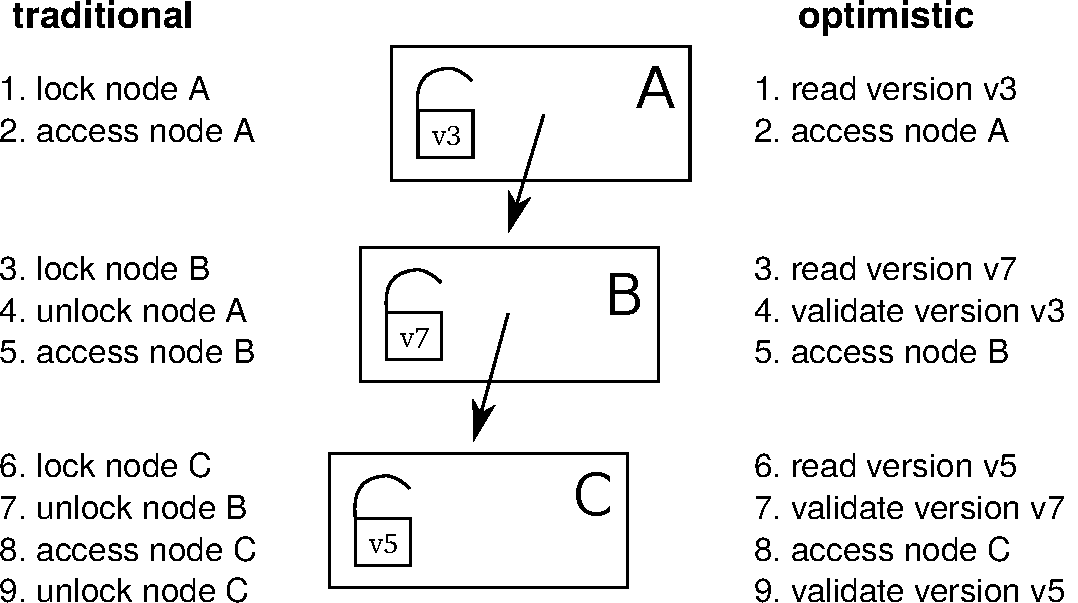
\includegraphics[width=0.65\linewidth]{olcall.pdf}
  \vspace{0.2cm}
  \caption{Comparison of a lookup operation in a 3-level tree using traditional lock coupling (left-hand side) vs.~optimistic lock coupling (right-hand side).}
  \label{fig:olc}
\end{figure}

The traditional and most common lock-based synchronization protocol for B-trees is lock coupling, which interleaves lock acquisitions while holding at most two locks at a time.
If, as we observed earlier, optimistic locks have similar semantics as traditional locks, it is natural to ask whether lock coupling can be combined with optimistic locks.
And indeed the answer is yes: One can almost mechanically translate traditional lock coupling code to optimistic lock coupling code.
This is illustrated in Figure~\ref{fig:olc}, which compares the traversal in a tree of height 3 using traditional and optimistic locks.
As the figure shows, the main difference is that locking is translated to reading the version and that unlocking becomes validation of the previously read version.
This simple change provides efficient lock-free tree traversal without the need to design a complex synchronization protocol.

It is important to emphasize the conceptual simplicity of OLC in comparison to data structures that use custom protocols like the Bw-tree~\cite{DBLP:conf/icde/LevandoskiLS13a}.
To implement lock-free access, the Bw-tree requires an indirection table, delta nodes, complex splitting and merging logic, retry logic, etc.
OLC, on the other hand, can directly be applied to B-trees mostly by adding the appropriate optimistic locking code and without modifying the node layout itself.
Therefore, OpenBw-Tree, an open source implementation of the Bw-tree, requires an order of magnitude more code than a B-tree based on OLC\footnote{Both implementations are available on GitHub: \url{https://github.com/wangziqi2016/index-microbench}}.
Given how difficult it is to develop, validate, and debug lock-free code, simplicity is obviously a major advantage.

\subsection{Correctness Aspects}

\begin{figure}
  % \centering
  %[basicstyle=\normalsize\ttfamily,showstringspaces=false,columns=fullflexible,breaklines=false,breakatwhitespace=true,numbers=none,numberstyle=\small,style=C,keepspaces=true]
\begin{lstlisting}[basicstyle=\ttfamily,language=C++,numbers=left,numberstyle=\small]
std::atomic<BTreeNode*> root;

// search for key in B+tree, returns payload in resultOut
bool lookup(Key key, Value& resultOut) {
   BTreeNode* node = root.load();
   uint64_t nodeVersion = node->readLockOrRestart();
   if (node != root.load()) // make sure the root is still the root
      restart();

   BTreeInner<Key>* parent = nullptr;
   uint64_t parentVersion = 0;

   while (node->isInner()) {
      auto inner = (BTreeInner*)node;

      // unlock parent and make current node the parent
      if (parent)
         parent->readUnlockOrRestart(parentVersion);
      parent = inner;
      parentVersion = nodeVersion;

      // search for next node
      node = inner->findChild(key);
      // validate 'inner' to ensure that 'node' pointer is valid
      inner->checkOrRestart(nodeVersion);
      // now it safe to dereference 'node' pointer (read its version)
      nodeVersion = node->readLockOrRestart();
   }

   // search in leaf and retrieve payload
   auto leaf = (BTreeLeaf*)node;
   bool success = leaf->findValue(key, resultOut);

   // unlock everything
   if (parent)
      parent->readUnlockOrRestart(parentVersion);
   node->readUnlockOrRestart(nodeVersion);

   return success;
}
\end{lstlisting}
  \vspace{0.2cm}
  \caption{B-tree lookup code using OLC. For simplicity, the restart logic is not shown.}
  \label{fig:lookup}
\end{figure}

So far, we have introduced the high-level ideas behind OLC and have stressed its similarity to traditional lock coupling.
Let us now discuss some cases where the close similarity between lock coupling and OLC breaks down.
To make this more concrete, we show the B-tree lookup code in Figure~\ref{fig:lookup}.
In the code, \texttt{readLockOrRestart} reads the lock version and \texttt{readUnlockOrRestart} validates that the read was correct.

One issue with OLC is that any pointer speculatively read from a node may point to invalid memory (if that node is modified concurrently).
Dereferencing such a pointer (e.g., to read its optimistic lock), may cause a segmentation fault or undefined behavior.
In the code shown in Figure~\ref{fig:lookup}, this problem is prevented by the extra check in line 25, which ensures that the read from the node containing the pointer was correct.
Without this additional validation, the code would in line 27 dereference the pointer speculatively read in line 23.
Note that the implementation of \texttt{checkOrRestart} is actually identical to \texttt{readUnlockOrRestart}.
We chose to give it a different name to highlight the fact that this extra check would not be necessary with read/write locks.

Another potential issue with optimistic locks is code that does not terminate.
Code that speculatively accesses a node, like an intra-node binary search, should be written in a way such that it always terminates---even in the presence of concurrent writes.
Otherwise, the validation code that detects the concurrent write will never run.
The binary search of a B-tree, for example, needs to be written in such a way that each comparison makes progress.
For some data structures that do not require loops in the traversal code (like ART) termination is trivially true.

\subsection{Implementation Details}

% implementation, efficiency
To implement an optimistic lock, one can combine the lock and the version counter into a single 64-bit\footnote{Even after subtracting one bit for the lock status, a back-of-the-envelope calculation can show that 63 bits are large enough to never overflow in practice.} word~\cite{artsync}.
A typical read operation will therefore merely consist of reading this version counter atomically.
In C++11 this can be implemented using the \texttt{std::atomic} type.

On x86, atomic reads are cheap because of x86's strong memory order guarantees.
No memory fences are required for sequentially-consistent loads, which are translated (by both GCC and clang) into standard \texttt{MOV} instructions.
Hence, the only effect of \texttt{std::atomic} for loads is preventing instruction re-ordering.
This makes version access and validation cheap.
Acquiring and releasing an optimistic lock in exclusive mode has comparable cost to a traditional lock:
A fairly expensive sequentially-consistent store is needed for acquiring a lock, while a standard \texttt{MOV} suffices for releasing it.
A simple sinlock-based implementation of optimistic locks can be found in the appendix of an earlier paper~\cite{artsync}.

OLC code must be able to handle restarts since validation or lock upgrade can fail due to concurrent writers.
Restarts can easily be implemented by wrapping the data structure operation in a loop (for simplicity not shown in Figure~\ref{fig:lookup}).
Such a loop also enables limiting the number of optimistic retry operations and falling back to pessimistic locking in cases of very heavy contention.
The ability to fall back to traditional locking is a major advantage of OLC in terms of robustness over lock-free approaches, which do not have this option.

In addition to the optimistic shared mode and the exclusive mode, optimistic locks also support a ``shared pessimistic'' mode, which physically acquires the lock in shared mode (allowing multiple concurrent readers but no writers).
This mode is useful for table (or range) scans that touch many tuples on a leaf page (which would otherwise easily abort).
Finally, let us mention that large range scans and table scans, should be broken up into several per-node traversals as is done in the LeanStore~\cite{leanstore} system.

Like all lock-free data structures, but unlike traditional locking and Hardware Transactional Memory~\cite{DBLP:conf/hpca/KarnagelDRLLSL14,DBLP:journals/pvldb/MakreshanskiLS15,htmtkde}, OLC requires care when deleting (and reusing) nodes.
The reason is that a deleting thread can never be sure that a node can be reclaimed because other threads might still be optimistically reading from that node.
Therefore, standard solutions like epoch-based reclamation~\cite{DBLP:conf/sosp/TuZKLM13}, hazard pointers~\cite{DBLP:journals/tpds/Michael04}, or optimized hazard pointers~\cite{DBLP:conf/spaa/BalmauGHZ16} need to be used.
These memory reclamation techniques are, however, largely orthogonal to the synchronization protocol itself.

%-lock-free is not a strong guarantee

\newpage
\section{Evaluation}\label{sec:evaluation}

Let us now experimentally evaluate the overhead and scalability of OLC.
For the experiments, we use an in-memory B+tree implemented in C++11 using templates, which is configured to use nodes of 4096 bytes, random 8 byte keys, and 8 byte payloads.
Based on this B-tree, we compare the following synchronization approaches:
\begin{itemize}
\item an OLC implementation\footnote{An almost identical OLC implementation is available on github: \url{https://github.com/wangziqi2016/index-microbench/tree/master/BTreeOLC}}
\item a variant based on traditional lock coupling and read/write locks
\item the unsynchronized B-tree, which obviously is only correct for read-only workloads but allows measuring the overhead of synchronization
\end{itemize}
Note that earlier work has compared the OLC implementation with a Bw-tree implementation~\cite{buzzword} and other state-of-the-art in-memory index structures.

We use a Haswell EP system with an Intel Xeon E5-2687W v3 CPU, which has 10 cores (20 ``Hyper-Threads'') and 25~MB of L3 cache.
The system is running Ubuntu 18.10 and we use GCC 8.2.0 to compile our code.
The CPU counters are obtained using the Linux perf API\footnote{We use the following convenience wrapper: \url{https://github.com/viktorleis/perfevent}}.

\begin{table}
  \caption{Performance and CPU counters for lookup and insert operations in a B-tree with 100M keys. We perform 100M operations and normalize the CPU counters by that number.}
  \label{tab:overhead}
  \centering
  \begin{tabular}{lrrrrrrr}\toprule
                    &         &        &        & instruc-  & L1     & L3     & branch \\
                    & threads & M op/s & cycles & tions & misses & misses & misses \\\midrule
lookup (no sync.)   & 1       & 1.72   & 2028   & 283     & 39.1   & 14.9   & 16.1   \\
lookup (OLC)        & 1       & 1.65   & 2107   & 370     & 43.9   & 15.1   & 16.7   \\
lookup (lock coup.) & 1       & 1.72   & 2078   & 365     & 42.3   & 16.9   & 15.7   \\\midrule
insert (no sync.)   & 1       & 1.51   & 2286   & 530     & 59.8   & 31.1   & 17.3   \\
insert (OLC)        & 1       & 1.50   & 2303   & 629     & 61.2   & 31.1   & 16.5   \\
insert (lock coup.) & 1       & 1.41   & 2473   & 644     & 61.0   & 31.0   & 17.2   \\\midrule
lookup (no sync.)   & 10      & 15.48  & 2058   & 283     & 38.6   & 15.5   & 16.0   \\
lookup (OLC)        & 10      & 14.60  & 2187   & 370     & 43.8   & 15.8   & 16.8   \\
lookup (lock coup.) & 10      & 5.71   & 5591   & 379     & 54.2   & 17.0   & 14.8   \\\midrule
insert (no sync.)   & 10      & -      & -      & -       & -      & -      & -      \\
insert (OLC)        & 10      & 10.46  & 2940   & 656     & 62.0   & 32.5   & 16.8   \\
insert (lock coup.) & 10      & 7.55   & 4161   & 667     & 75.0   & 28.6   & 16.2   \\
    \bottomrule
\end{tabular}
\end{table}

Table~\ref{tab:overhead} compares the performance and CPU counters for lookup and insert operations in a B-tree with 100M keys.
With {\em single-threaded} execution, we observe that all three approaches have very similar performance.
Adding traditional or optimistic locks to unsynchronized B-tree code results in up to 30\% of additional instructions without affecting single-threaded performance much.

\begin{figure}
  \centering
  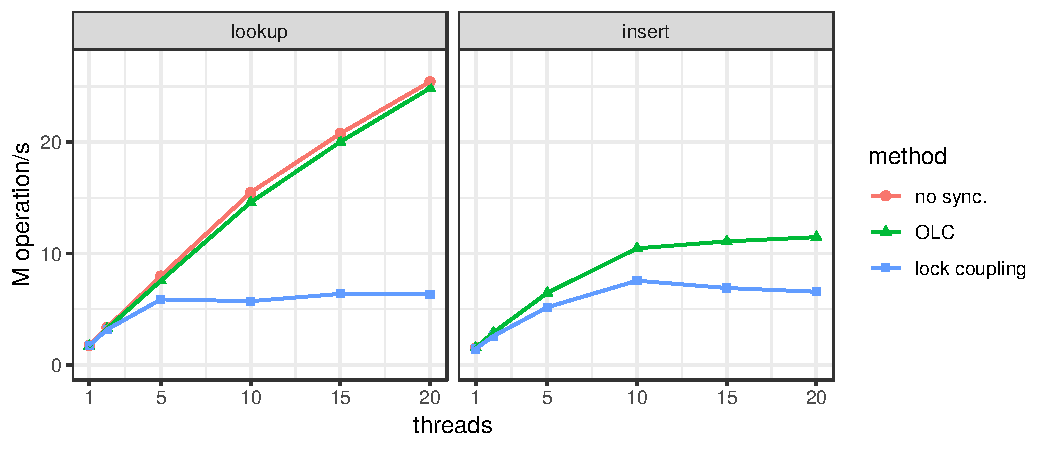
\includegraphics[width=\linewidth]{scale.pdf}
  \vspace{0.2cm}
  \caption{Scalability on 10-core system for B-tree operations (100M values).}
  \label{fig:scale}
\end{figure}

As Figure~\ref{fig:scale} shows, the results change dramatically once we use multiple threads.
For lookup, the scalability of OLC is near-linear up to 20 threads, even though the system has only 10 ``real cores''.
The OLC scalability for insert is also respectable (though not quite as linear because multi-threaded insertion approaches the memory bandwidth of our processor).
The figure also shows that the results of traditional lock coupling with read/write locks are significantly worse than OLC.
With 20 threads, lookup with OLC is 3.9$\times$ faster than traditional lock coupling.

\section{Summary}\label{sec:conc}

Optimistic Lock Coupling (OLC) is an effective synchronization method that combines the simplicity of traditional lock coupling with the superior scalability of lock-free approaches.
OLC is widely applicable and has already been successfully used to synchronize several data structures, including B-trees, binary search trees, and different trie variants.
These features make it highly attractive for modern database systems as well as performance-critical systems software in general.

\begin{thebibliography}{10}

\bibitem{DBLP:conf/spaa/BalmauGHZ16}
O.~Balmau, R.~Guerraoui, M.~Herlihy, and I.~Zablotchi.
\newblock Fast and robust memory reclamation for concurrent data structures.
\newblock In {\em SPAA}, 2016.

\bibitem{DBLP:journals/acta/BayerS77}
R.~Bayer and M.~Schkolnick.
\newblock Concurrency of operations on {B}-trees.
\newblock {\em Acta Informatica}, 9, 1977.

\bibitem{hot}
R.~Binna, E.~Zangerle, M.~Pichl, G.~Specht, and V.~Leis.
\newblock {HOT}: A height optimized trie index for main-memory database
  systems.
\newblock In {\em SIGMOD}, 2018.

\bibitem{DBLP:conf/ppopp/BronsonCCO10}
N.~G. Bronson, J.~Casper, H.~Chafi, and K.~Olukotun.
\newblock A practical concurrent binary search tree.
\newblock In {\em PPOPP}, 2010.

\bibitem{DBLP:conf/vldb/ChaHKK01}
S.~K. Cha, S.~Hwang, K.~Kim, and K.~Kwon.
\newblock Cache-conscious concurrency control of main-memory indexes on
  shared-memory multiprocessor systems.
\newblock In {\em VLDB}, 2001.

\bibitem{intel}
I.~Cutress.
\newblock {Intel} goes for 48-cores: {Cascade-AP} with multi-chip package
  coming soon.
\newblock
  \url{https://www.anandtech.com/show/13535/intel-goes-for-48cores-cascade-ap},
  2018 (accessed January, 2019).

\bibitem{DBLP:conf/cidr/FaleiroA17}
J.~M. Faleiro and D.~J. Abadi.
\newblock Latch-free synchronization in database systems: Silver bullet or
  fool's gold?
\newblock In {\em CIDR}, 2017.

\bibitem{DBLP:journals/ftdb/Graefe11}
G.~Graefe.
\newblock Modern {B}-tree techniques.
\newblock {\em Foundations and Trends in Databases}, 3(4), 2011.

\bibitem{DBLP:conf/hpca/KarnagelDRLLSL14}
T.~Karnagel, R.~Dementiev, R.~Rajwar, K.~Lai, T.~Legler, B.~Schlegel, and
  W.~Lehner.
\newblock Improving in-memory database index performance with
  {Intel}\({}^{\mbox{{\textregistered}}}\) transactional synchronization
  extensions.
\newblock In {\em HPCA}, 2014.

\bibitem{DBLP:journals/tods/LehmanY81}
P.~L. Lehman and S.~B. Yao.
\newblock Efficient locking for concurrent operations on {B}-trees.
\newblock {\em {ACM} Trans. Database Syst.}, 6(4), 1981.

\bibitem{leanstore}
V.~Leis, M.~Haubenschild, A.~Kemper, and T.~Neumann.
\newblock Leanstore: In-memory data management beyond main memory.
\newblock In {\em ICDE}, 2018.

\bibitem{art}
V.~Leis, A.~Kemper, and T.~Neumann.
\newblock The adaptive radix tree: {ARTful} indexing for main-memory databases.
\newblock In {\em ICDE}, 2013.

\bibitem{htmtkde}
V.~Leis, A.~Kemper, and T.~Neumann.
\newblock Scaling {HTM}-supported database transactions to many cores.
\newblock {\em {IEEE} Trans. Knowl. Data Eng.}, 28(2), 2016.

\bibitem{artsync}
V.~Leis, F.~Scheibner, A.~Kemper, and T.~Neumann.
\newblock The {ART} of practical synchronization.
\newblock In {\em DaMoN}, 2016.

\bibitem{DBLP:conf/icde/LevandoskiLS13a}
J.~J. Levandoski, D.~B. Lomet, and S.~Sengupta.
\newblock The {Bw}-tree: A {B}-tree for new hardware platforms.
\newblock In {\em ICDE}, 2013.

\bibitem{DBLP:journals/pvldb/MakreshanskiLS15}
D.~Makreshanski, J.~J. Levandoski, and R.~Stutsman.
\newblock To lock, swap, or elide: On the interplay of hardware transactional
  memory and lock-free indexing.
\newblock {\em {PVLDB}}, 8(11), 2015.

\bibitem{DBLP:dblp_conf/eurosys/MaoKM12}
Y.~Mao, E.~Kohler, and R.~T. Morris.
\newblock Cache craftiness for fast multicore key-value storage.
\newblock In {\em EuroSys}, 2012.

\bibitem{DBLP:journals/tpds/Michael04}
M.~M. Michael.
\newblock Hazard pointers: Safe memory reclamation for lock-free objects.
\newblock {\em {IEEE} Trans. Parallel Distrib. Syst.}, 15(6), 2004.

\bibitem{DBLP:journals/jacm/ShalevS06}
O.~Shalev and N.~Shavit.
\newblock Split-ordered lists: Lock-free extensible hash tables.
\newblock {\em J. {ACM}}, 53(3), 2006.

\bibitem{amd}
A.~Shilov.
\newblock {AMD} previews {EPYC} ‘{Rome}’ processor: Up to 64 {Zen} 2 cores.
\newblock
  \url{https://www.anandtech.com/show/13561/amd-previews-epyc-rome-processor-up-to-64-zen-2-cores},
  2018 (accessed January, 2019).

\bibitem{DBLP:conf/sosp/TuZKLM13}
S.~Tu, W.~Zheng, E.~Kohler, B.~Liskov, and S.~Madden.
\newblock Speedy transactions in multicore in-memory databases.
\newblock In {\em SOSP}, 2013.

\bibitem{buzzword}
Z.~Wang, A.~Pavlo, H.~Lim, V.~Leis, H.~Zhang, M.~Kaminsky, and D.~Andersen.
\newblock Building a {Bw}-tree takes more than just buzz words.
\newblock In {\em SIGMOD}, 2018.

\end{thebibliography}


%\bibliographystyle{abbrv}
%\bibliography{main}

\end{document}
 
\end{article}
\begin{article}
{Does Differential Privacy Impact Bias in Pretrained Language Models?}
{Md. Khairul Islam, Andrew Wang, Tianhao Wang, Yangfeng Ji, Judy Fox, Jieyu Zhao}
\pdfminorversion=5
\documentclass[11pt]{article}
\usepackage{deauthor,times,graphicx,caption,microtype}
\usepackage{hyperref}
\usepackage{listings}
\usepackage{booktabs}

\begin{document}

\title{Optimistic Lock Coupling: A Scalable and Efficient General-Purpose Synchronization Method}

\author{Viktor Leis, Michael Haubenschild\raisebox{0.9ex}{$\ast$}, Thomas Neumann\\ Technische Universit{\"a}t M{\"u}nchen \hspace{0.7cm} Tableau Software\raisebox{0.9ex}{$\ast$} \\ {\{leis,neumann\}{@}in.tum.de} \hspace{0.7cm} {mhaubenschild{@}tableau.com\raisebox{0.9ex}{$\ast$}}}

\maketitle

\begin{abstract}
As the number of cores on commodity processors continues to increase, scalability becomes more and more crucial for overall performance.
Scalable and efficient concurrent data structures are particularly important, as these are often the building blocks of parallel algorithms.
Unfortunately, traditional synchronization techniques based on fine-grained locking have been shown to be unscalable on modern multi-core CPUs.
Lock-free data structures, on the other hand, are extremely difficult to design and often incur significant overhead.

In this work, we make the case for Optimistic Lock Coupling as a practical alternative to both traditional locking and the lock-free approach.
We show that Optimistic Lock Coupling is highly scalable and almost as simple to implement as traditional lock coupling.
Another important advantage is that it is easily applicable to most tree-like data structures.
We therefore argue that Optimistic Lock Coupling, rather than a complex and error-prone custom synchronization protocol, should be the default choice for performance-critical data structures.
\end{abstract}

\section{Introduction}

% more and more cores
Today, Intel's commodity server processors have up to 28 cores and its upcoming microarchitecture will have up to 48 cores per socket~\cite{intel}.
Similarly, AMD currently stands at 32 cores and this number is expected to double in the next generation~\cite{amd}.
Since both platforms support simultaneous multithreading (also known as hyperthreading), affordable commodity servers (with up to two sockets) will soon routinely have between 100 and 200 hardware threads.

% data structure scalability is important
With such a high degree of hardware parallelism, efficient data processing crucially depends on how well concurrent data structures scale.
Internally, database systems use a plethora of data structures like table heaps, internal work queues, and, most importantly, index structures.
Any of these can easily become a scalability (and therefore overall performance) bottleneck on many-core CPUs.

% traditional synchronization: fine-grained locks, slow, cache invalidation
Traditionally, database systems synchronize internal data structures using fine-grained reader/writer locks\footnote{In this work, we focus on data structure synchronization rather than high-level transaction semantics and therefore use the term {\em lock} for what would typically be called {\em latch} in the database literature. We thus follow common computer science (rather than database) terminology.}.
Unfortunately, while fine-grained locking makes lock contention unlikely, it still results in bad scalability because lock acquisition and release require writing to shared memory.
Due to the way cache coherency is implemented on modern multi-core CPUs, these writes cause additional cache misses\footnote{The cache coherency protocol ensures that all copies of a cache line on other cores are invalidated before the write can proceed.} and the cache line containing the lock's internal data becomes a point of physical contention.
As a result, any frequently-accessed lock (e.g., the lock of the root node of a B-tree) severely limits scalability.

% lock-free bw-tree: no more latches, but indirections, extremely complex
Lock-free data structures like the Bw-tree~\cite{DBLP:conf/icde/LevandoskiLS13a} (a lock-free B-tree variant) or the Split-Ordered List~\cite{DBLP:journals/jacm/ShalevS06} (a lock-free hash table) do not acquire any locks and therefore generally scale much better than locking-based approaches (in particular for read-mostly workloads).
However, lock-free synchronization has other downsides:
First, it is very difficult and results in extremely complex and error-prone code (when compared to locking).
Second, because the functionality of atomic primitives provided by the hardware (e.g., atomically compare-and-swap 8 bytes) is limited, complex operations require additional indirections within the data structure.
For example, the Bw-tree requires an indirection table and the Split-Ordered List requires ``dummy nodes'', resulting in overhead due to additional cache misses.

% OLC for the win
In this paper we make the case for {\em Optimistic Lock Coupling (OLC)}, a synchronization method that combines some of the best properties of lock-based and lock-free synchronization.
OLC utilizes a special lock type that can be used in two modes:
The first mode is similar to a traditional mutex and excludes other threads by physically acquiring the underlying lock.
In the second mode, reads can proceed optimistically by validating a version counter that is embedded in the lock (similar to optimistic concurrency control).
The first mode is typically used by writers and the second mode by readers.
Besides this special lock type, OLC is based on the observation that optimistic lock validations can be interleaved/coupled---similar to the pair-wise interleaved lock acquisition of traditional lock coupling.
Hence, the name Optimistic Lock Coupling.

OLC has a number of desirable features:
\begin{itemize}
\item By reducing the number of writes to shared memory locations and thereby avoiding cache invalidations, it {\bf scales well} for most workloads.
\item In comparison to unsynchronized code, it requires few additional CPU instructions making it {\bf efficient}.
\item OLC is {\bf widely applicable} to different data structures. It has already been successfully used for synchronizing binary search trees~\cite{DBLP:conf/ppopp/BronsonCCO10}, tries~\cite{artsync}, trie/B-tree hybrids~\cite{DBLP:dblp_conf/eurosys/MaoKM12}, and B-trees~\cite{buzzword}.
\item In comparison to the lock-free paradigm, it is also {\bf easy to use} and requires few modifications to existing, single-threaded data structures.
\end{itemize}
Despite these positive features and its simplicity, OLC is not yet widely known.
The goal of this paper is therefore to popularize this simple idea and to make a case for it.
We argue that OLC deserves to be widely known.
It is a good default synchronization paradigm---more complex, data structure-specific protocols are seldom beneficial.

The rest of the paper is organized as follows.
Section~\ref{sec:related} discusses related work, tracing the history of OLC and its underlying ideas in the literature.
The core of the paper is Section~\ref{sec:olc}, which describes the ideas behind OLC and how it can be used to synchronize complex data structures.
In Section~\ref{sec:evaluation} we experimentally show that OLC has low overhead and scales well when used to synchronize an in-memory B-tree.
We summarize the paper in Section~\ref{sec:conc}.

\newpage
\section{Related Work}\label{sec:related}

Lock coupling has been proposed as a method for allowing concurrent operations on B-trees in 1977~\cite{DBLP:journals/acta/BayerS77}.
This traditional and still widely-used method, described in detail in Graefe's B-tree survey~\cite{DBLP:journals/ftdb/Graefe11}, is also called ``latch coupling'', ``hand-over-hand locking'', and ``crabbing''.
Because at most two locks are held at-a-time during tree traversal, this technique seemingly allows for a high degree of parallelism---in particular if read/write locks are used to enable inner nodes to be locked in shared mode.
However, as we show in Section~\ref{sec:evaluation}, on modern hardware lock acquisition (even in shared mode) results in suboptimal scalability.

An early alternative from 1981 is a B-tree variant called B-link tree~\cite{DBLP:journals/tods/LehmanY81}, which only holds a single lock at a time.
It is based on the observation that between the release of the parent lock and the acquisition of the child lock, the only ``dangerous'' thing that could have happened is the split of a child node (assuming one does not implement merge operations).
Thus, when a split happens, the key being searched might end up on a neighboring node to the right of the current child node.
A B-link tree traversal therefore detects this condition and, if needed, transparently proceeds to the neighboring node.
Releasing the parent lock early is highly beneficial when the child node needs to be fetched from disk.
For in-memory workloads, however, the B-link tree has the same scalability issues as lock coupling (it acquires just as many locks).

The next major advance, Optimistic Latch-Free Index Traversal (OLFIT)~\cite{DBLP:conf/vldb/ChaHKK01}, was proposed in 2001.
OLFIT introduced the idea of a combined lock/update counter, which we call {\em optimistic lock}. % , for lack of a better name,
Based on these per-node optimistic locks and the synchronization protocol of the B-link tree, OLFIT finally achieves good scalability on parallel processors.
The OLFIT protocol is fairly complex, as it requires both the non-trivial B-link protocol and optimistic locks.
Furthermore, like the B-link tree protocol, it does not support merging nodes, and is specific to B-trees (cannot easily be applied to other data structures).

In the following two decades, the growth of main-memory capacity led to much research into other data structures besides the venerable B-tree.
Particularly relevant for our discussion is Bronson et al.'s~\cite{DBLP:conf/ppopp/BronsonCCO10} concurrent binary search tree, which is based on optimistic version validation and has a sophisticated, data structure-specific synchronization protocol.
To the best of our knowledge, this 2010 paper is the first that, as part of its protocol, interleaves version validation across nodes---rather than validating each node separately like OLFIT.
In that paper, this idea is called ``hand-over-hand, optimistic validation'', while we prefer the term Optimistic Lock Coupling to highlight the close resemblance to traditional lock coupling.
Similarly, Mao et al.'s~\cite{DBLP:dblp_conf/eurosys/MaoKM12} Masstree (a concurrent hybrid trie/B-tree) is also based on the same ideas, but again uses them as part of a more complex protocol.

The Adaptive Radix Tree (ART)~\cite{art} is another recent in-memory data structure, which we proposed in 2013.
In contrast to the two data structures just mentioned, it was originally designed with single-threaded performance in mind without supporting concurrency.
To add support for concurrency, we initially started designing a custom protocol called Read-Optimized Write Exclusion (ROWEX)~\cite{artsync}, which turned out to be non-trivial and requires modifications of the underlying data structure\footnote{Note that ROWEX is already easier to apply to existing data structures than the lock-free approach. The difficulty depends on the data structure. Applying ROWEX is hard for B-trees with sorted keys and fairly easy for copy-on-write data structures like the Height Optimized Trie~\cite{hot}---with ART being somewhere in the middle.}.
However, fairly late in the project, we also realized, that OLC {\em alone} (rather than as part of a more complex protocol) is sufficient to synchronize ART.
No other changes to the data structure were necessary.
Both approaches were published and experimentally evaluated in a followup paper~\cite{artsync}, which shows that, despite its simplicity, OLC is efficient, scalable, and generally outperforms ROWEX.

Similar results were recently published regarding B-trees~\cite{buzzword}.
In this experimental study a simple OLC-based synchronization outperformed the Bw-tree~\cite{DBLP:conf/icde/LevandoskiLS13a}, a complex lock-free synchronization approach.
Another recent paper shows that for write-intensive workloads, locking often performs better than lock-free synchronization~\cite{DBLP:conf/cidr/FaleiroA17}.
These experiences indicate that OLC is a general-purpose synchronization paradigm and motivate the current paper.

%foster b-tree\cite{DBLP:journals/tods/GraefeKK12}
%Shasha theory~\cite{DBLP:journals/tods/ShashaG88}

\section{Optimistic Lock Coupling}\label{sec:olc}

% locks suck
The standard technique for inter-thread synchronization is mutual exclusion using fine-grained locks.
In a B-tree, for example, every node usually has its own associated lock, which is acquired before accessing that node.
The problem of locking on modern multi- and many-core processors is that lock acquisition and release require writing to the shared memory location that implements the lock.
This write causes exclusive ownership of the underlying cache line and invalidates copies of it on all other processor cores.
For hierarchical, tree-like data structures, the lock of the root node becomes a point of physical contention---even in read-only workloads and even when read/write locks are used.
Depending on the specific data structure, number of cores, cache coherency protocol implementation, cache topology, whether Non-Uniform Memory Access (NUMA) is used, locking can even result in multi-threaded performance that is worse than single-threaded execution.

% in b-trees this happens very much
The inherent pessimism of locking is particularly unfortunate for B-trees:
Despite the fact that logical modifications of the root node are very infrequent, every B-tree operation must lock the root node during tree traversal\footnote{To a lesser extent this obviously applies to all inner nodes, not just the root.}.
Even the vast majority of update operations (with the exception of splits and merges), only modify a single leaf node.
These observations indicate that a more optimistic approach, which does not require locking inner nodes, would be very beneficial for B-trees.

\subsection{Optimistic Locks}

% optimism to the rescue
As the name indicates, optimistic locks try to solve the scalability issues of traditional locks using an optimistic approach.
Instead of always physically acquiring locks, even for nodes that are unlikely to be modified simultaneously, after-the-fact validation is used to detect conflicts.
This is done by augmenting each lock with a version/update counter that is incremented on every modification.
Using this version counter, readers can optimistically proceed before validating that the version did not change to ensure that the read was safe.
If validation fails, the operation is restarted.

% details on opt locks
Using optimistic locks, a read-only node access (i.e., the majority of all operations in a B-tree) does not acquire the lock and does not increment the version counter.
Instead, it performs the following steps:
\begin{enumerate}
\item read lock version (restart if lock is not free)
\item access node
\item read the version again and validate that it has not changed in the meantime
\end{enumerate}
If the last step (the validation) fails, the operation has to be restarted.
Write operations, on the other hand, are more similar to traditional locking:
\begin{enumerate}
\item acquire lock (wait if necessary)
\item access/write to node
\item increment version and unlock node
\end{enumerate}
Writes can therefore protect a node from other writes.

% similar to locks
As we observed in an earlier paper~\cite{artsync}, because of similar semantics, optimistic locks can be hidden behind an API very similar to traditional read/write locks.
Both approaches have an exclusive lock mode, and acquiring a traditional lock in shared mode is analogous to optimistic version validation.
Furthermore, like with some implementations of traditional read/write locks, optimistic locks allow upgrading a shared lock to an exclusive lock.
Lock upgrades are, for example, used to avoid most B-tree update operations from having to lock inner nodes.
In our experience, the close resemblance of optimistic and traditional locks simplifies the reasoning about optimistic locks;
one can apply similar thinking as in traditional lock-based protocols.

\subsection{Lock Coupling with Optimistic Locks}

\begin{figure}
  \centering
  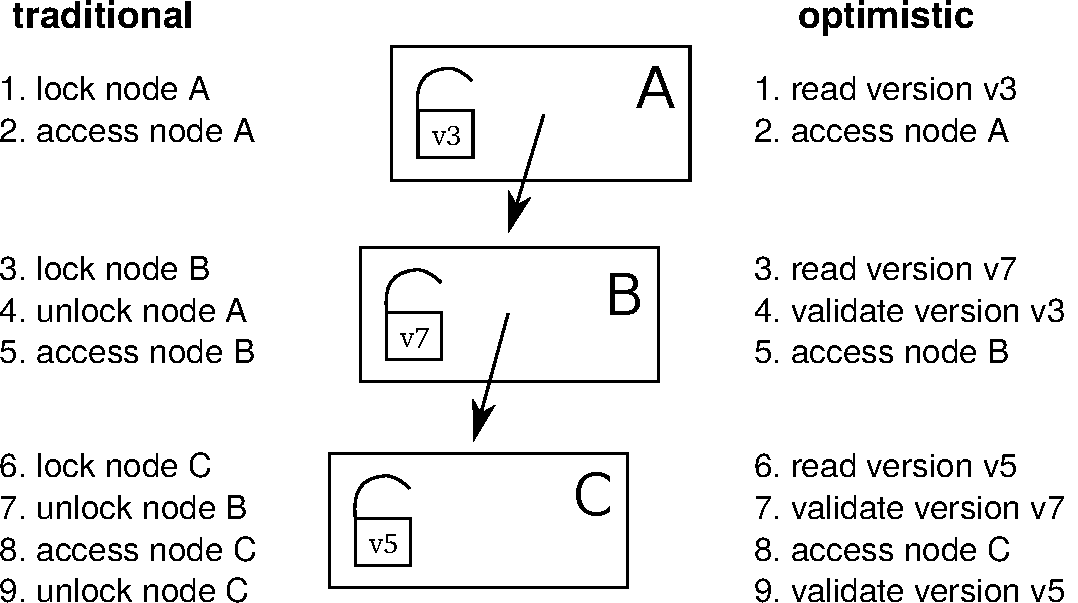
\includegraphics[width=0.65\linewidth]{olcall.pdf}
  \vspace{0.2cm}
  \caption{Comparison of a lookup operation in a 3-level tree using traditional lock coupling (left-hand side) vs.~optimistic lock coupling (right-hand side).}
  \label{fig:olc}
\end{figure}

The traditional and most common lock-based synchronization protocol for B-trees is lock coupling, which interleaves lock acquisitions while holding at most two locks at a time.
If, as we observed earlier, optimistic locks have similar semantics as traditional locks, it is natural to ask whether lock coupling can be combined with optimistic locks.
And indeed the answer is yes: One can almost mechanically translate traditional lock coupling code to optimistic lock coupling code.
This is illustrated in Figure~\ref{fig:olc}, which compares the traversal in a tree of height 3 using traditional and optimistic locks.
As the figure shows, the main difference is that locking is translated to reading the version and that unlocking becomes validation of the previously read version.
This simple change provides efficient lock-free tree traversal without the need to design a complex synchronization protocol.

It is important to emphasize the conceptual simplicity of OLC in comparison to data structures that use custom protocols like the Bw-tree~\cite{DBLP:conf/icde/LevandoskiLS13a}.
To implement lock-free access, the Bw-tree requires an indirection table, delta nodes, complex splitting and merging logic, retry logic, etc.
OLC, on the other hand, can directly be applied to B-trees mostly by adding the appropriate optimistic locking code and without modifying the node layout itself.
Therefore, OpenBw-Tree, an open source implementation of the Bw-tree, requires an order of magnitude more code than a B-tree based on OLC\footnote{Both implementations are available on GitHub: \url{https://github.com/wangziqi2016/index-microbench}}.
Given how difficult it is to develop, validate, and debug lock-free code, simplicity is obviously a major advantage.

\subsection{Correctness Aspects}

\begin{figure}
  % \centering
  %[basicstyle=\normalsize\ttfamily,showstringspaces=false,columns=fullflexible,breaklines=false,breakatwhitespace=true,numbers=none,numberstyle=\small,style=C,keepspaces=true]
\begin{lstlisting}[basicstyle=\ttfamily,language=C++,numbers=left,numberstyle=\small]
std::atomic<BTreeNode*> root;

// search for key in B+tree, returns payload in resultOut
bool lookup(Key key, Value& resultOut) {
   BTreeNode* node = root.load();
   uint64_t nodeVersion = node->readLockOrRestart();
   if (node != root.load()) // make sure the root is still the root
      restart();

   BTreeInner<Key>* parent = nullptr;
   uint64_t parentVersion = 0;

   while (node->isInner()) {
      auto inner = (BTreeInner*)node;

      // unlock parent and make current node the parent
      if (parent)
         parent->readUnlockOrRestart(parentVersion);
      parent = inner;
      parentVersion = nodeVersion;

      // search for next node
      node = inner->findChild(key);
      // validate 'inner' to ensure that 'node' pointer is valid
      inner->checkOrRestart(nodeVersion);
      // now it safe to dereference 'node' pointer (read its version)
      nodeVersion = node->readLockOrRestart();
   }

   // search in leaf and retrieve payload
   auto leaf = (BTreeLeaf*)node;
   bool success = leaf->findValue(key, resultOut);

   // unlock everything
   if (parent)
      parent->readUnlockOrRestart(parentVersion);
   node->readUnlockOrRestart(nodeVersion);

   return success;
}
\end{lstlisting}
  \vspace{0.2cm}
  \caption{B-tree lookup code using OLC. For simplicity, the restart logic is not shown.}
  \label{fig:lookup}
\end{figure}

So far, we have introduced the high-level ideas behind OLC and have stressed its similarity to traditional lock coupling.
Let us now discuss some cases where the close similarity between lock coupling and OLC breaks down.
To make this more concrete, we show the B-tree lookup code in Figure~\ref{fig:lookup}.
In the code, \texttt{readLockOrRestart} reads the lock version and \texttt{readUnlockOrRestart} validates that the read was correct.

One issue with OLC is that any pointer speculatively read from a node may point to invalid memory (if that node is modified concurrently).
Dereferencing such a pointer (e.g., to read its optimistic lock), may cause a segmentation fault or undefined behavior.
In the code shown in Figure~\ref{fig:lookup}, this problem is prevented by the extra check in line 25, which ensures that the read from the node containing the pointer was correct.
Without this additional validation, the code would in line 27 dereference the pointer speculatively read in line 23.
Note that the implementation of \texttt{checkOrRestart} is actually identical to \texttt{readUnlockOrRestart}.
We chose to give it a different name to highlight the fact that this extra check would not be necessary with read/write locks.

Another potential issue with optimistic locks is code that does not terminate.
Code that speculatively accesses a node, like an intra-node binary search, should be written in a way such that it always terminates---even in the presence of concurrent writes.
Otherwise, the validation code that detects the concurrent write will never run.
The binary search of a B-tree, for example, needs to be written in such a way that each comparison makes progress.
For some data structures that do not require loops in the traversal code (like ART) termination is trivially true.

\subsection{Implementation Details}

% implementation, efficiency
To implement an optimistic lock, one can combine the lock and the version counter into a single 64-bit\footnote{Even after subtracting one bit for the lock status, a back-of-the-envelope calculation can show that 63 bits are large enough to never overflow in practice.} word~\cite{artsync}.
A typical read operation will therefore merely consist of reading this version counter atomically.
In C++11 this can be implemented using the \texttt{std::atomic} type.

On x86, atomic reads are cheap because of x86's strong memory order guarantees.
No memory fences are required for sequentially-consistent loads, which are translated (by both GCC and clang) into standard \texttt{MOV} instructions.
Hence, the only effect of \texttt{std::atomic} for loads is preventing instruction re-ordering.
This makes version access and validation cheap.
Acquiring and releasing an optimistic lock in exclusive mode has comparable cost to a traditional lock:
A fairly expensive sequentially-consistent store is needed for acquiring a lock, while a standard \texttt{MOV} suffices for releasing it.
A simple sinlock-based implementation of optimistic locks can be found in the appendix of an earlier paper~\cite{artsync}.

OLC code must be able to handle restarts since validation or lock upgrade can fail due to concurrent writers.
Restarts can easily be implemented by wrapping the data structure operation in a loop (for simplicity not shown in Figure~\ref{fig:lookup}).
Such a loop also enables limiting the number of optimistic retry operations and falling back to pessimistic locking in cases of very heavy contention.
The ability to fall back to traditional locking is a major advantage of OLC in terms of robustness over lock-free approaches, which do not have this option.

In addition to the optimistic shared mode and the exclusive mode, optimistic locks also support a ``shared pessimistic'' mode, which physically acquires the lock in shared mode (allowing multiple concurrent readers but no writers).
This mode is useful for table (or range) scans that touch many tuples on a leaf page (which would otherwise easily abort).
Finally, let us mention that large range scans and table scans, should be broken up into several per-node traversals as is done in the LeanStore~\cite{leanstore} system.

Like all lock-free data structures, but unlike traditional locking and Hardware Transactional Memory~\cite{DBLP:conf/hpca/KarnagelDRLLSL14,DBLP:journals/pvldb/MakreshanskiLS15,htmtkde}, OLC requires care when deleting (and reusing) nodes.
The reason is that a deleting thread can never be sure that a node can be reclaimed because other threads might still be optimistically reading from that node.
Therefore, standard solutions like epoch-based reclamation~\cite{DBLP:conf/sosp/TuZKLM13}, hazard pointers~\cite{DBLP:journals/tpds/Michael04}, or optimized hazard pointers~\cite{DBLP:conf/spaa/BalmauGHZ16} need to be used.
These memory reclamation techniques are, however, largely orthogonal to the synchronization protocol itself.

%-lock-free is not a strong guarantee

\newpage
\section{Evaluation}\label{sec:evaluation}

Let us now experimentally evaluate the overhead and scalability of OLC.
For the experiments, we use an in-memory B+tree implemented in C++11 using templates, which is configured to use nodes of 4096 bytes, random 8 byte keys, and 8 byte payloads.
Based on this B-tree, we compare the following synchronization approaches:
\begin{itemize}
\item an OLC implementation\footnote{An almost identical OLC implementation is available on github: \url{https://github.com/wangziqi2016/index-microbench/tree/master/BTreeOLC}}
\item a variant based on traditional lock coupling and read/write locks
\item the unsynchronized B-tree, which obviously is only correct for read-only workloads but allows measuring the overhead of synchronization
\end{itemize}
Note that earlier work has compared the OLC implementation with a Bw-tree implementation~\cite{buzzword} and other state-of-the-art in-memory index structures.

We use a Haswell EP system with an Intel Xeon E5-2687W v3 CPU, which has 10 cores (20 ``Hyper-Threads'') and 25~MB of L3 cache.
The system is running Ubuntu 18.10 and we use GCC 8.2.0 to compile our code.
The CPU counters are obtained using the Linux perf API\footnote{We use the following convenience wrapper: \url{https://github.com/viktorleis/perfevent}}.

\begin{table}
  \caption{Performance and CPU counters for lookup and insert operations in a B-tree with 100M keys. We perform 100M operations and normalize the CPU counters by that number.}
  \label{tab:overhead}
  \centering
  \begin{tabular}{lrrrrrrr}\toprule
                    &         &        &        & instruc-  & L1     & L3     & branch \\
                    & threads & M op/s & cycles & tions & misses & misses & misses \\\midrule
lookup (no sync.)   & 1       & 1.72   & 2028   & 283     & 39.1   & 14.9   & 16.1   \\
lookup (OLC)        & 1       & 1.65   & 2107   & 370     & 43.9   & 15.1   & 16.7   \\
lookup (lock coup.) & 1       & 1.72   & 2078   & 365     & 42.3   & 16.9   & 15.7   \\\midrule
insert (no sync.)   & 1       & 1.51   & 2286   & 530     & 59.8   & 31.1   & 17.3   \\
insert (OLC)        & 1       & 1.50   & 2303   & 629     & 61.2   & 31.1   & 16.5   \\
insert (lock coup.) & 1       & 1.41   & 2473   & 644     & 61.0   & 31.0   & 17.2   \\\midrule
lookup (no sync.)   & 10      & 15.48  & 2058   & 283     & 38.6   & 15.5   & 16.0   \\
lookup (OLC)        & 10      & 14.60  & 2187   & 370     & 43.8   & 15.8   & 16.8   \\
lookup (lock coup.) & 10      & 5.71   & 5591   & 379     & 54.2   & 17.0   & 14.8   \\\midrule
insert (no sync.)   & 10      & -      & -      & -       & -      & -      & -      \\
insert (OLC)        & 10      & 10.46  & 2940   & 656     & 62.0   & 32.5   & 16.8   \\
insert (lock coup.) & 10      & 7.55   & 4161   & 667     & 75.0   & 28.6   & 16.2   \\
    \bottomrule
\end{tabular}
\end{table}

Table~\ref{tab:overhead} compares the performance and CPU counters for lookup and insert operations in a B-tree with 100M keys.
With {\em single-threaded} execution, we observe that all three approaches have very similar performance.
Adding traditional or optimistic locks to unsynchronized B-tree code results in up to 30\% of additional instructions without affecting single-threaded performance much.

\begin{figure}
  \centering
  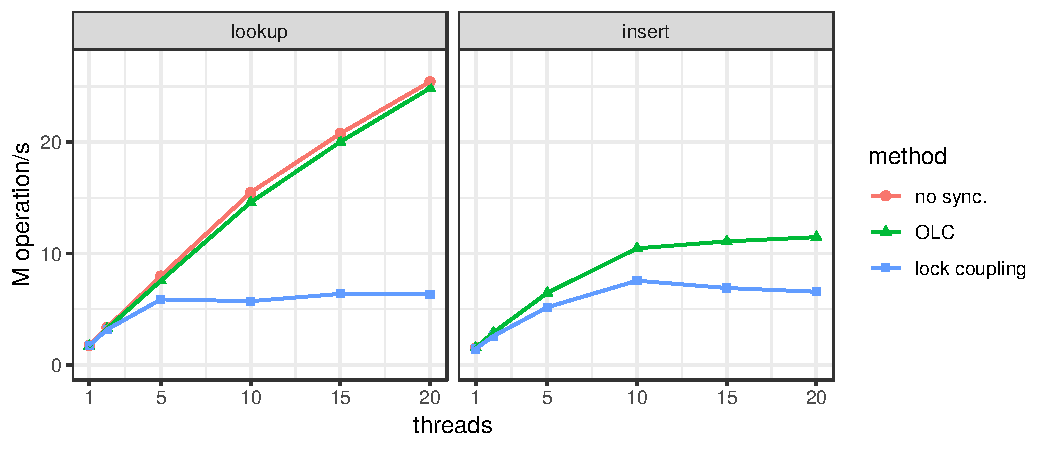
\includegraphics[width=\linewidth]{scale.pdf}
  \vspace{0.2cm}
  \caption{Scalability on 10-core system for B-tree operations (100M values).}
  \label{fig:scale}
\end{figure}

As Figure~\ref{fig:scale} shows, the results change dramatically once we use multiple threads.
For lookup, the scalability of OLC is near-linear up to 20 threads, even though the system has only 10 ``real cores''.
The OLC scalability for insert is also respectable (though not quite as linear because multi-threaded insertion approaches the memory bandwidth of our processor).
The figure also shows that the results of traditional lock coupling with read/write locks are significantly worse than OLC.
With 20 threads, lookup with OLC is 3.9$\times$ faster than traditional lock coupling.

\section{Summary}\label{sec:conc}

Optimistic Lock Coupling (OLC) is an effective synchronization method that combines the simplicity of traditional lock coupling with the superior scalability of lock-free approaches.
OLC is widely applicable and has already been successfully used to synchronize several data structures, including B-trees, binary search trees, and different trie variants.
These features make it highly attractive for modern database systems as well as performance-critical systems software in general.

\begin{thebibliography}{10}

\bibitem{DBLP:conf/spaa/BalmauGHZ16}
O.~Balmau, R.~Guerraoui, M.~Herlihy, and I.~Zablotchi.
\newblock Fast and robust memory reclamation for concurrent data structures.
\newblock In {\em SPAA}, 2016.

\bibitem{DBLP:journals/acta/BayerS77}
R.~Bayer and M.~Schkolnick.
\newblock Concurrency of operations on {B}-trees.
\newblock {\em Acta Informatica}, 9, 1977.

\bibitem{hot}
R.~Binna, E.~Zangerle, M.~Pichl, G.~Specht, and V.~Leis.
\newblock {HOT}: A height optimized trie index for main-memory database
  systems.
\newblock In {\em SIGMOD}, 2018.

\bibitem{DBLP:conf/ppopp/BronsonCCO10}
N.~G. Bronson, J.~Casper, H.~Chafi, and K.~Olukotun.
\newblock A practical concurrent binary search tree.
\newblock In {\em PPOPP}, 2010.

\bibitem{DBLP:conf/vldb/ChaHKK01}
S.~K. Cha, S.~Hwang, K.~Kim, and K.~Kwon.
\newblock Cache-conscious concurrency control of main-memory indexes on
  shared-memory multiprocessor systems.
\newblock In {\em VLDB}, 2001.

\bibitem{intel}
I.~Cutress.
\newblock {Intel} goes for 48-cores: {Cascade-AP} with multi-chip package
  coming soon.
\newblock
  \url{https://www.anandtech.com/show/13535/intel-goes-for-48cores-cascade-ap},
  2018 (accessed January, 2019).

\bibitem{DBLP:conf/cidr/FaleiroA17}
J.~M. Faleiro and D.~J. Abadi.
\newblock Latch-free synchronization in database systems: Silver bullet or
  fool's gold?
\newblock In {\em CIDR}, 2017.

\bibitem{DBLP:journals/ftdb/Graefe11}
G.~Graefe.
\newblock Modern {B}-tree techniques.
\newblock {\em Foundations and Trends in Databases}, 3(4), 2011.

\bibitem{DBLP:conf/hpca/KarnagelDRLLSL14}
T.~Karnagel, R.~Dementiev, R.~Rajwar, K.~Lai, T.~Legler, B.~Schlegel, and
  W.~Lehner.
\newblock Improving in-memory database index performance with
  {Intel}\({}^{\mbox{{\textregistered}}}\) transactional synchronization
  extensions.
\newblock In {\em HPCA}, 2014.

\bibitem{DBLP:journals/tods/LehmanY81}
P.~L. Lehman and S.~B. Yao.
\newblock Efficient locking for concurrent operations on {B}-trees.
\newblock {\em {ACM} Trans. Database Syst.}, 6(4), 1981.

\bibitem{leanstore}
V.~Leis, M.~Haubenschild, A.~Kemper, and T.~Neumann.
\newblock Leanstore: In-memory data management beyond main memory.
\newblock In {\em ICDE}, 2018.

\bibitem{art}
V.~Leis, A.~Kemper, and T.~Neumann.
\newblock The adaptive radix tree: {ARTful} indexing for main-memory databases.
\newblock In {\em ICDE}, 2013.

\bibitem{htmtkde}
V.~Leis, A.~Kemper, and T.~Neumann.
\newblock Scaling {HTM}-supported database transactions to many cores.
\newblock {\em {IEEE} Trans. Knowl. Data Eng.}, 28(2), 2016.

\bibitem{artsync}
V.~Leis, F.~Scheibner, A.~Kemper, and T.~Neumann.
\newblock The {ART} of practical synchronization.
\newblock In {\em DaMoN}, 2016.

\bibitem{DBLP:conf/icde/LevandoskiLS13a}
J.~J. Levandoski, D.~B. Lomet, and S.~Sengupta.
\newblock The {Bw}-tree: A {B}-tree for new hardware platforms.
\newblock In {\em ICDE}, 2013.

\bibitem{DBLP:journals/pvldb/MakreshanskiLS15}
D.~Makreshanski, J.~J. Levandoski, and R.~Stutsman.
\newblock To lock, swap, or elide: On the interplay of hardware transactional
  memory and lock-free indexing.
\newblock {\em {PVLDB}}, 8(11), 2015.

\bibitem{DBLP:dblp_conf/eurosys/MaoKM12}
Y.~Mao, E.~Kohler, and R.~T. Morris.
\newblock Cache craftiness for fast multicore key-value storage.
\newblock In {\em EuroSys}, 2012.

\bibitem{DBLP:journals/tpds/Michael04}
M.~M. Michael.
\newblock Hazard pointers: Safe memory reclamation for lock-free objects.
\newblock {\em {IEEE} Trans. Parallel Distrib. Syst.}, 15(6), 2004.

\bibitem{DBLP:journals/jacm/ShalevS06}
O.~Shalev and N.~Shavit.
\newblock Split-ordered lists: Lock-free extensible hash tables.
\newblock {\em J. {ACM}}, 53(3), 2006.

\bibitem{amd}
A.~Shilov.
\newblock {AMD} previews {EPYC} ‘{Rome}’ processor: Up to 64 {Zen} 2 cores.
\newblock
  \url{https://www.anandtech.com/show/13561/amd-previews-epyc-rome-processor-up-to-64-zen-2-cores},
  2018 (accessed January, 2019).

\bibitem{DBLP:conf/sosp/TuZKLM13}
S.~Tu, W.~Zheng, E.~Kohler, B.~Liskov, and S.~Madden.
\newblock Speedy transactions in multicore in-memory databases.
\newblock In {\em SOSP}, 2013.

\bibitem{buzzword}
Z.~Wang, A.~Pavlo, H.~Lim, V.~Leis, H.~Zhang, M.~Kaminsky, and D.~Andersen.
\newblock Building a {Bw}-tree takes more than just buzz words.
\newblock In {\em SIGMOD}, 2018.

\end{thebibliography}


%\bibliographystyle{abbrv}
%\bibliography{main}

\end{document}
 
\end{article}
\end{articlesection}

% put the news items below- there can be multiple news sections
% each with its own title
% news will usually have an author as well as a title,
% e.g. TCDE elections
% news articles are in the same format as letters
% typically, news articles will be stored in a directory called "news"


% \begin{newssection}{Obituary}
% \begin{news}{Obituary for Professor Gio Wiederhold}
% {Kyu-Young Whang and Marianne Winslett}{Distinguished Professor Emeritus, KAIST\\ Research Professor Emerita, UIUC\\ together with Gio’s other former students}
% \documentclass[11pt]{article} 

\usepackage{deauthor,times,graphicx}
%\usepackage{url}
\usepackage{hyperref}

\begin{document}
%Obituary for Professor Gio Wiederhold
%                                                                  December 26, 2022                                                                         
Professor Gio Wiederhold passed away in the early hours of December 26, 2022, aged 86, just 10 weeks after an unexpected diagnosis of stage 4 liver cancer. Gio died at home, surrounded by his family members who had gathered for Christmas, including his wife of 56 years, Voy Wiederhold, and his sons John and Randy.  


Gio was a great scholar, educator, and mentor. His influence on the database field is immense. As a pioneer in the database field, he wrote the influential 1977 textbook Database Design, one of the first in the field and adopted around the world. In his DARPA-supported Knowledge-Base Management Systems project in the early 1980s, Gio pioneered the concept of integrating databases and AI, a topic that is now enjoying a revival. Beginning in the 1970s, Gio also pursued the application of databases to medical informatics, another area just now entering the mainstream. In 1992, Gio introduced the notion of mediators (IEEE Computer) as a way of intelligently integrating information from large-scale heterogeneous sources such as databases, file systems, and repositories, a seminal idea for the nascent field of information integration. Gio continued to innovate after retirement from Stanford, most notably in establishing an approach for valuing software and the intellectual property of multinational firms.


Gio advised 36 PhD students at Stanford. Today, Gio’s academic descendants can be found in companies and universities all over the world, including early students Hector Garcia-Molina (the late Stanford professor), David Shaw (DE Shaw founder), Ramez Elmasri (the late textbook author and UT Arlington professor), Kyu-Young Whang (KAIST professor and Naver founder’s advisor), and Marianne Winslett (UIUC professor). Gio’s many subsequent students continue to lead the database field today. 


An influential mentor, Gio always emphasized the practical aspects of research, encouraging people to develop both theoretical and engineering approaches to solve real-world problems. This outlook stemmed from his many years of experience in computing practice before he joined the Stanford University faculty.


Gio’s service to the professional community includes serving as the third Editor-in-Chief of ACM Transactions on Databases during 1985-1995, during which time he significantly contributed to making the new journal a top one in the field. Together with five colleagues, Gio co-founded the IEEE International Conference on Data Engineering in 1984. Perhaps the first venue to use the term data engineering, the conference was unique in focusing on engineering aspects of database research; today it stands as one of the three top-tier conferences in database research. Gio also served as the conference’s program committee chair, co-chair, and general chair in its early years. During 1991-1994, Gio served as the program manager for DARPA’s Knowledge-based Systems program, which collaborated with NSF to fund innovative new research related to information integration and digital libraries — including the project that led to the creation of Google.


In recognition of his many contributions, Gio received the IEEE Technical Community on Data Engineering’s Service Award in 2016. He was also a Fellow of the ACM, the IEEE, and the American College of Medical Informatics.




The many accomplishments and contributions listed above do not capture the full extent of Gio’s impact and influence on our community, nor his diligence and persistence. As Gio’s former students, we dearly miss him for his warm heart towards his students, colleagues, and friends, and above all, his love and kindness for everyone he knew. We are deeply saddened by Gio’s unexpected death and send our sincerest condolences to his surviving family and friends.  




%-- Kyu-Young Whang, Distinguished Professor Emeritus, KAIST and Marianne Winslett, Research Professor Emerita, University of Illinois at Urbana-Champaign, together with Gio’s other former students
\end{document}

% \end{news}

% \newpage
% \end{newssection}


\begin{callsection}

%  This section will be empty for your version
%
%  Calls for papers section.  Use the callsection environment.
%  Each call for papers is contained in an call environment, where the single
%  required options to \begin{call} is the name of the conference.
% typically calls are stored in a "calls" directory
%
%\begin{call}{name of conference}
%\centerline{\includegraphics[width=\textwidth, bb= 0 0 590 760]{calls/conference-name.pdf}}
%\end{call}
%\begin{call}{ICDE 2019 Conference}
%\centerline{
\includegraphics[width=\textwidth, bb= 0 0 610 790] {../Dec-2018/calls/icde19.pdf}}
%\centerline{
\includegraphics[width=\textwidth, bb= 0 0 590 760] {calls/icde19.pdf}}
%\end{call}
\begin{call}{TCDE Membership Form}
%\centerline{\includegraphics[width=\textwidth, bb= 0 0 610 790]
%\centerline{
\includegraphics[width=\textwidth, bb= 0 0 590 760] {../Dec-2018/calls/tcde.pdf}}
\centerline{
\includegraphics[width=\textwidth, bb= 0 0 590 760] {./calls/tcde.pdf}}
\end{call}

\end{callsection}

\end{bulletin}
\end{document}
